\section{Analytická geometrie v rovině}
\label{sec:Analytic_geometry_plane}

V této kapitole se budeme zabývat geometrickými útvary v rovině
a jejich popisem pomocí souřadnic, vektorů a rovnic. Nejprve se
zaměříme na přímky, které patří mezi základní objekty analytické
geometrie.

Ukážeme si několik způsobů, kterými lze tutéž přímku vyjádřit,
naučíme se mezi těmito způsoby převádět a následně budeme zkoumat
vzájemnou polohu dvou přímek.

\subsection{Úvod k přímkám v rovině}
\label{subsec:Lines_in_plane}

Přímku v rovině lze popsat několika různými způsoby. Každý z nich
zdůrazňuje jinou její vlastnost a může být výhodný v jiném typu úloh.

Parametrické vyjádření pracuje s bodem přímky a jejím směrovým
vektorem. Obecná rovnice využívá normálový vektor, zatímco směrnicový
tvar popisuje nesvislou přímku pomocí její směrnice a průsečíku
s osou $y$.

V následujících částech postupně zavedeme všechny tři způsoby zápisu
a vysvětlíme jejich geometrický význam.

\subsection{Parametrické vyjádření přímky}
\label{subsec:Parametric_line}

Parametrické vyjádření přímky je založeno na myšlence,
že přímka může být popsána pomocí bodu, kterým prochází, a směru, kterým se táhne.
Toto vyjádření je velmi intuitivní a často se používá v praxi,
zejména v počítačové grafice a fyzice.

\begin{remark}
    V počítačové grafice se parametrické vyjádření přímky často používá k 
    interpolaci mezi dvěma body nebo k popisu trajektorie pohybu.
    Ve fyzice se zase využívá k popisu pohybu částic nebo k modelování silových polí.
\end{remark}

Protože víme, že přímka je určitý druh čáry, rovné čáry, která 
nemá žádné zakřivení a táhne se nekonečně daleko v obou směrech.
A protože již víme, že pomocí vektoru můžeme popsat směr a zároveň
se můžeme díky násobkům vektoru posouvat dále, či blíže od počátečního bodu,
můžeme přímku popsat pomocí směrového vektoru a bodu, kterým prochází.

\begin{definition}\label{def:Parametric_line}
    Nechť $A$ je bod v rovině a $\vec{u}$ je nenulový vektor.
    Pak přímka $p$ procházející bodem $A$ a směrem určeným směrovým vektorem $\vec{u}$ může být vyjádřena jako množina všech bodů $X$, které lze získat jako
    \begin{equation}
        X = A + t\vec{u}, \quad t \in \mathbb{R}.
    \end{equation}
    Rozšířením této rovnice do souřadnic získáme parametrické rovnice přímky:
    \begin{equation}
        \begin{aligned}
            x &= x_A + t u_x, \\
            y &= y_A + t u_y,
            \qquad t \in \mathbb{R}.
        \end{aligned}
        \label{eq:Parametric_line_coordinate_form}
    \end{equation}
    kde $A[x_A; y_A]$ jsou souřadnice bodu $A$ a $\vec{u} = (u_x; u_y)$ jsou souřadnice směrového vektoru $\vec{u}$.

    Tento způsob vyjádření přímky se nazývá \textbf{parametrické vyjádření přímky}.
\end{definition}

V tomto vyjádření je $t$ nazýván \textbf{parametrem} přímky.
Mění-li se $t$, mění se i bod $X$ na přímce, a tím pádem můžeme získat všechny body na přímce.
Pro $t=0$ získáme bod $A$, který jsme zvolili jako jeden pevný bod přímky.
Přímka sama nemá žádný počáteční ani koncový bod, protože se neomezeně
rozprostírá v obou směrech.
Když $t$ je kladné, získáme body na přímce ve směru vektoru $\vec{u}$, a když $t$ je záporné, získáme body na přímce v opačném směru.

\begin{figure}[H]
    \centering
    \begin{tikzpicture}[scale=1]

        % Bod A
        \coordinate (A) at (1,2);
        \fill (A) circle (2pt) node[right] {$A[1,2]$};

        % Směrový vektor
        \coordinate (U) at (3,4);
        \draw[vector] (A) -- (U) node[midway, above left] {$\vec{u}$};

        % Přímka (prodloužení směru)
        \draw[thin] (-1,0) -- (5,6) node[right] {$p$};

    \end{tikzpicture}
    \caption{Parametrické vyjádření přímky $p$ dané bodem $A$ a vektorem $\vec{u}$.}
    \label{fig:Parametric_line}
\end{figure}

\begin{remark}
    Směrový vektor přímky není určen jednoznačně. Je-li $\vec{u}$
    směrovým vektorem přímky, potom je jejím směrovým vektorem také
    každý jeho nenulový reálný násobek
    \[
        k\cdot\vec{u},\qquad k\in\mathbb{R}\setminus\{0\}.
    \]
    Všechny tyto vektory jsou navzájem rovnoběžné, a určují proto
    stejný směr přímky.
\end{remark}

Z této skutečnosti zároveň plyne, že ani parametrické vyjádření přímky
není jednoznačné. Pro tutéž přímku můžeme zvolit kterýkoli její bod
a kterýkoli nenulový směrový vektor rovnoběžný s přímkou.

Například zápisy
\begin{align*}
    p: x &= 1+2t,\\
       y &= 2+2t;\quad t\in\mathbb{R},
\end{align*}
a
\begin{align*}
    p: x &= 3-4s,\\
       y &= 4-4s;\quad s\in\mathbb{R}
\end{align*}
popisují tutéž přímku. Druhý zápis totiž používá bod $[3;4]$, který
na původní přímce leží, a směrový vektor $(-4;-4)$, jenž je násobkem
původního směrového vektoru $(2;2)$.

\begin{example}
    Mějme bod $A[1; 2]$ a vektor $\vec{u} = (2; 2)$.
    Najděme parametrické vyjádření přímky $p$, která prochází bodem $A$ a má směr určený vektorem $\vec{u}$.

    Podle definice \ref{def:Parametric_line} můžeme přímku $p$ vyjádřit jako
    \begin{align*}
        X   &= A + t\vec{u} \\
            &= [1; 2] + t(2; 2) \\
            &= [1 + 2t; 2 + 2t], \quad t \in \mathbb{R}.
    \end{align*}

    Což můžeme zapsat následujícími způsoby:
    \begin{align*}
        p:  x &= 1 + 2t, \\
            y &= 2 + 2t; \quad t \in \mathbb{R}.
    \end{align*}

    Případně můžeme využít zápis pomocí množin:
    \[
        p = \{ [x; y] \in \mathbb{R}^2 \mid x = 1 + 2t, y = 2 + 2t, t \in \mathbb{R} \},
    \]
    nebo:
    \[
        p = \{ [1 + 2t; 2 + 2t] ; t \in \mathbb{R} \}.
    \]

    Všechny tři způsoby zápisu jsou ekvivalentní a popisují stejnou přímku $p$ v rovině.
\end{example}

\begin{example}
    Mějme parametrické vyjádření přímky $q$ dané jako:
    \begin{align*}
        q:  x &= 3 + 4t, \\
            y &= 1 - t; \quad t \in \mathbb{R}.
    \end{align*}
    Najděme bod, kterým přímka $q$ prochází, a vektor, který určuje její směr.

    Z parametrického vyjádření přímky $q$ můžeme snadno určit bod, kterým prochází, a vektor, který určuje její směr.
    Bod $B$ je dán hodnotami $x$ a $y$ pro $t=0$:
    \[
        B = [3 + 4 \cdot 0; 1 - 0] = [3; 1].
    \]
    Souřadnice jednoho bodu přímky tedy získáme z konstantních členů parametrických rovnic, zatímco souřadnice směrového vektoru tvoří koeficienty u parametru $t$.
    Vektor $\vec{v}$, který určuje směr přímky $q$, je dán koeficienty u $t$ v rovnicích pro $x$ a $y$:
    \[
        \vec{v} = (4; -1).
    \]
    Můžeme tedy opět rovnou určit vektor $\vec{v}$ tak, že vezmeme koeficienty u $t$ z obou rovnic.
    
    Tedy přímka $q$ prochází bodem $B[3; 1]$ a má směr určený vektorem $\vec{v} = (4; -1)$.
\end{example}

\begin{example}
    Zjistěte hodnoty dalších bodů na přímce $p$ z prvního příkladu pro různé hodnoty parametru $t$.
    \begin{align*}
        p : x &= 1 + 2t, \\
            y &= 2 + 2t; \quad t \in \mathbb{R}.
    \end{align*}

    Pro zjištění dalších bodů na přímce $p$ můžeme dosadit různé hodnoty parametru $t$ do rovnic pro $x$ a $y$,
    a získat tak souřadnice dalších bodů na přímce.

    Pro $t = 1$:
    \begin{align*}
        x &= 1 + 2 \cdot 1 = 3, \\
        y &= 2 + 2 \cdot 1 = 4.
    \end{align*}
    Tedy bod $C$ na přímce $p$ pro $t=1$ je $C[3; 4]$.

    Pro $t = -1$:
    \begin{align*}
        x &= 1 + 2 \cdot (-1) = -1, \\
        y &= 2 + 2 \cdot (-1) = 0.
    \end{align*}
    Tedy bod $D$ na přímce $p$ pro $t=-1$ je $D[-1; 0]$.

    Pro $t = 0.5$:
    \begin{align*}
        x &= 1 + 2 \cdot \tfrac{1}{2} = 2, \\
        y &= 2 + 2 \cdot \tfrac{1}{2} = 3.
    \end{align*}
    Tedy bod $E$ na přímce $p$ pro $t=\frac{1}{2}$ je $E[2; 3]$.
\end{example}

\begin{example}\label{exa:Points_on_parametric_line}
    Zjistěte, zda-li body $F[5; 6]$ a $G[0; 0]$ leží na přímce $p$, která je dána parametrickým vyjádřením:
    \begin{align*}
        p : x &= 1 + 2t, \\
            y &= 2 + 2t; \quad t \in \mathbb{R}.
    \end{align*}

    Pro zjištění, zda-li bod $F[5; 6]$ leží na přímce $p$, musíme zjistit, zda existuje hodnota parametru $t$, pro kterou platí rovnice pro $x$ a $y$.
    Dosadíme tedy souřadnice bodu $F$ do rovnic pro $x$ a $y$ a zjistíme, zda-li existuje společné řešení pro $t$.

    \begin{align*}
        5 &= 1 + 2t \quad \Rightarrow \quad 2t = 4 \quad \Rightarrow \quad t = 2, \\
        6 &= 2 + 2t \quad \Rightarrow \quad 2t = 4 \quad \Rightarrow \quad t = 2.
    \end{align*}

    Pro $t=2$ platí obě rovnice, tedy bod $F[5; 6]$ leží na přímce $p$.

    Pro zjištění, zda-li bod $G[0; 0]$ leží na přímce $p$, opět dosadíme souřadnice bodu $G$ do rovnic pro $x$ a $y$ a zjistíme, zda-li existuje společné řešení pro $t$.
    \begin{align*}
        0 &= 1 + 2t \quad \Rightarrow \quad 2t = -1 \quad \Rightarrow \quad t = -\frac{1}{2}, \\
        0 &= 2 + 2t \quad \Rightarrow \quad 2t = -2 \quad \Rightarrow \quad t = -1.
    \end{align*}
    Pro $x$ a $y$ získáváme různé hodnoty pro $t$, tedy neexistuje žádná hodnota parametru $t$, pro kterou by platily obě rovnice, a proto bod $G[0; 0]$ neleží na přímce $p$.

\end{example}

V příkladu \ref{exa:Points_on_parametric_line} jsme zjistili, že bod
$F[5;6]$ na přímce $p$ leží, protože pro obě jeho souřadnice vyšla
stejná hodnota parametru $t=2$. Naopak pro bod $G[0;0]$ jsme z první
rovnice získali $t=-\frac12$, zatímco z druhé rovnice $t=-1$.
Neexistuje tedy jediná hodnota parametru, která by současně vytvořila
obě souřadnice bodu $G$.

Stejnou skutečnost můžeme vysvětlit také pomocí vektorů. Vektor směřující
z bodu $A[1;2]$ do bodu $G[0;0]$ je
\[
    \overrightarrow{AG}=(0-1;0-2)=(-1;-2).
\]
Aby bod $G$ ležel na přímce $p$, musel by být vektor
$\overrightarrow{AG}$ reálným násobkem směrového vektoru
$\vec{u}=(2;2)$. To však neplatí, protože neexistuje číslo
$k\in\mathbb{R}$, pro které by současně platilo
\[
    (-1;-2)=k(2;2).
\]
Vektory $\overrightarrow{AG}$ a $\vec{u}$ nejsou rovnoběžné, a proto
bod $G$ na přímce $p$ neleží.

\begin{figure}[H]
    \centering
    \begin{tikzpicture}[scale=0.8]

        % Body
        \coordinate (A) at (1,2);
        \coordinate (F) at (5,6);
        \coordinate (G) at (0,0);

        \fill (A) circle (2pt) node[right] {$A[1; 2]$};
        \fill (F) circle (2pt) node[right] {$F[5; 6]$};
        \fill (G) circle (2pt) node[left] {$G[0; 0]$};

        % Směrový vektor u
        \coordinate (U) at (3,4);
        \draw[vector] (A) -- (U) node[midway, above left] {$\vec{u}$};

        % Vektor k bodu G (není rovnoběžný)
        \draw[vector, dashed] (A) -- (G) node[midway, below] {$\vec{v}$};

        % Přímka
        \draw[thin] (0,1) -- (6,7) node[right] {$p$};

    \end{tikzpicture}
    \caption{Bod $F$ leží na přímce $p$, zatímco bod $G$ neleží na přímce $p$.}
    \label{fig:Parametric_line_points}
\end{figure}

Zatím jsme přímku v rovině ještě neurčovali, ale zasipovali jsme ji pomocí bodu a směrového vektoru.
Jak jsme si ukázali, tak bod na přímce je dán souřadnicemi, které získáme dosazením hodnot za parametry (násobky směrového vektoru) do parametrické rovnice přímky.
Tedy pokud chceme přímku v rovině určit, tak potřebujeme bod a směrový vektor, který určuje směr přímky (viz definice \ref{def:Parametric_line}).
Můžeme tedy dopočítat i parametrické vyjádření přímky, pokud máme dva body, které na přímce leží.

V dosavadních příkladech jsme znali bod přímky a její směrový vektor. Často jsou však zadány dva různé body $A[x_A;y_A]$ a $B[x_B;y_B]$, kterými má přímka procházet. Protože dvěma různými body v rovině prochází právě jedna přímka, získáme její směrový vektor jako
\[
    \overrightarrow{AB}=(x_B-x_A;y_B-y_A).
\]
Parametrické vyjádření potom můžeme sestavit ve tvaru
\begin{equation}\label{eq:Parametric_line_two_points}
    X=A+t\overrightarrow{AB},\qquad t\in\mathbb{R},
\end{equation}

Geometrický význam vztahu \eqref{eq:Parametric_line_two_points}
je znázorněn na obrázku \ref{fig:Parametric_line_two_points}.
Z bodu $A$ se pomocí různých reálných násobků vektoru
$\overrightarrow{AB}$ můžeme pohybovat po celé přímce v obou směrech.

\begin{figure}[H]
    \centering
    \begin{tikzpicture}[scale=1]

        % Body
        \coordinate (A) at (0,0);
        \coordinate (B) at (3,2);

        % Přímka
        \draw[thin] (-1,-0.67) -- (5,3.33) node[right] {$p$};

        % Body A a B
        \fill (A) circle (2pt) node[below right] {$A$};
        \fill (B) circle (2pt) node[below right] {$B$};

        % Směrový vektor
        \draw[vector] (A) -- (B)
            node[midway, above left] {$\overrightarrow{AB}$};

    \end{tikzpicture}
    \caption{Přímka $p$ určená dvěma různými body $A$ a $B$ a směrovým vektorem $\overrightarrow{AB}$.}
    \label{fig:Parametric_line_two_points}
\end{figure}

Parametrické rovnice přímky tedy po rozepsání souřadnic znamená
\begin{align}
    x &= x_A+t(x_B-x_A),\\
    y &= y_A+t(y_B-y_A);\quad t\in\mathbb{R}.
\end{align}

Můžeme tedy upravit definici \ref{def:Parametric_line} tak, že přímku určíme dvěma body, kterými prochází.
\begin{definition}
    Nechť $A$ a $B$ jsou dva různé body v rovině. Pak přímka $p$ procházející body $A$ a $B$ může být vyjádřena jako množina všech bodů $X$, které lze získat jako
    \begin{equation}
        X = A + t\overrightarrow{AB}, \quad t \in \mathbb{R}.
    \end{equation}
    Rozšířením této rovnice do souřadnic získáme parametrické rovnice přímky:
    \begin{equation}
        \begin{aligned}
            x &= x_A + t(x_B - x_A), \\
            y &= y_A + t(y_B - y_A),
            \qquad t \in \mathbb{R}.
        \end{aligned}
        \label{eq:Parametric_line_two_points_coordinate_form}
    \end{equation}
    Tento způsob vyjádření přímky se nazývá \textbf{parametrické vyjádření přímky určené dvěma body}.
\end{definition}


\begin{example}\label{exa:Parametric_line_from_two_points}
    Mějte dva body $H[2; 3]$ a $I[5; 7]$.
    Najděte parametrické vyjádření přímky $r$, která prochází těmito dvěma body.

    Nejprve určíme směrový vektor $\vec{w}$ přímky $r$ jako vektor směřující z bodu $H$ do bodu $I$:
    \[
        \vec{w} = \overrightarrow{HI} = (5 - 2; 7 - 3) = (3; 4).
    \]

    Nyní můžeme použít bod $H$ a směrový vektor $\vec{w}$ k vytvoření parametrického vyjádření přímky $r$:
    \begin{align*}
        r: x &= 2 + 3t, \\
           y &= 3 + 4t; \quad t \in \mathbb{R}.
    \end{align*}

    Tedy parametrické vyjádření přímky $r$, která prochází body $H[2; 3]$ a $I[5; 7]$, je dáno výše uvedenými rovnicemi.
    Geometrický princip tohoto postupu je znázorněn na obrázku \ref{fig:Parametric_line_two_points}.
\end{example}

Zatím jsme řešili pouze přímky v rovině, ale pomocí změny hodnot parametru $t$ můžeme získat i jiné rovinné útvary, například \textbf{úsečky} a \textbf{polopřímky}.
Využijeme příklad \ref{exa:Parametric_line_from_two_points}, kde jsme získali parametrické vyjádření přímky $r$ procházející body $H[2; 3]$ a $I[5; 7]$.

\begin{example}\label{exa:Parametric_ray_through_two_points}
    Určete parametrické vyjádření polopřímky $\overrightarrow{HI}$
    z příkladu \ref{exa:Parametric_line_from_two_points}, která začíná
    bodem $H$ a prochází bodem $I$.

    Polopřímka $\overrightarrow{HI}$ začíná v bodě $H$ a pokračuje
    neomezeně daleko ve směru bodu $I$. Nejprve určíme vektor
    \[
        \overrightarrow{HI}
        =(5-2;7-3)
        =(3;4).
    \]

    Použijeme-li bod $H[2;3]$ a směrový vektor
    $\overrightarrow{HI}=(3;4)$, získáme parametrické vyjádření
    přímky procházející body $H$ a $I$:
    \begin{align*}
        r: x &= 2+3t,\\
           y &= 3+4t;\quad t\in\mathbb{R}.
    \end{align*}

    Chceme-li však popsat pouze polopřímku $\overrightarrow{HI}$,
    musíme parametr omezit na nezáporné hodnoty. Pro $t=0$ získáme
    počáteční bod $H$, pro $t=1$ bod $I$ a pro $t>1$ body ležící
    za bodem $I$ ve stejném směru.

    První parametrické vyjádření polopřímky tedy je
    \begin{align*}
        r_1: x &= 2+3t,\\
             y &= 3+4t;
             \quad t\in\langle 0;+\infty).
    \end{align*}

    Tutéž polopřímku můžeme popsat také pomocí opačně orientovaného
    vektoru
    \[
        \overrightarrow{IH}
        =(2-5;3-7)
        =(-3;-4).
    \]

    V tomto případě je vhodné použít jako pevný bod bod $I[5;7]$.
    Dostáváme tedy
    \begin{align*}
        r_2: x &= 5-3t,\\
             y &= 7-4t.
    \end{align*}

    Pro $t=1$ získáme bod
    \[
        [5-3;7-4]=[2;3]=H,
    \]
    zatímco pro $t=0$ získáme bod $I$. Abychom získali také všechny
    body ležící za bodem $I$ ve směru polopřímky $\overrightarrow{HI}$,
    musíme připustit všechny hodnoty $t\leq 1$.

    Druhé parametrické vyjádření téže polopřímky proto je
    \begin{align*}
        r_2: x &= 5-3t,\\
             y &= 7-4t;
             \quad t\in(-\infty;1\rangle.
    \end{align*}

    Geometrické znázornění polopřímky $\overrightarrow{HI}$ je uvedeno na obrázku \ref{fig:Parametric_ray_HI}. 
    Je na něm patrné, že bod $H$ je počátečním bodem polopřímky, zatímco bod $I$ určuje směr jejího dalšího pokračování.
\end{example}

\begin{figure}[H]
    \centering
    \begin{tikzpicture}[scale=0.65]

        % Body polopřímky
        \coordinate (H) at (2,3);
        \coordinate (I) at (5,7);
        \coordinate (R) at (7.25,10);

        % Polopřímka
        \draw[thin, ->] (H) -- (R);

        % Body H a I
        \fill (H) circle (2.5pt) node[below right] {$H[2;3]$};
        \fill (I) circle (2.5pt) node[below right] {$I[5;7]$};

        % Směrový vektor
        \draw[vector] (H) -- (I)
            node[midway, above, sloped] {$\vec{w}$};

        % Označení pokračování
        \node[below right] at (R) {$\overrightarrow{HI}$};

    \end{tikzpicture}
    \caption{Polopřímka $\overrightarrow{HI}$ začíná v bodě $H$, prochází bodem $I$ a pokračuje neomezeně daleko ve směru bodu $I$}
    \label{fig:Parametric_ray_HI}
\end{figure}

Oba zápisy z příkladu
\ref{exa:Parametric_ray_through_two_points} popisují tutéž polopřímku
$\overrightarrow{HI}$, přestože používají jiný pevný bod, opačně
orientované směrové vektory a jiný obor hodnot parametru.

Ekvivalenci obou zápisů můžeme ověřit substitucí
\[
    s=1-t.
\]
Protože ve druhém zápisu platí $t\leq 1$, dostáváme
\[
    s\geq 0.
\]

Dosadíme-li $t=1-s$ do druhého parametrického vyjádření, získáme
\begin{align*}
    x &= 5-3(1-s)
       =5-3+3s
       =2+3s,\\
    y &= 7-4(1-s)
       =7-4+4s
       =3+4s.
\end{align*}

Tedy
\begin{align*}
    x &= 2+3s,\\
    y &= 3+4s;
    \quad s\in\langle0;+\infty),
\end{align*}
což je právě první parametrické vyjádření polopřímky
$\overrightarrow{HI}$.


Nyní se zaměříme na úsečku $\overline{HI}$. Zatímco přímka procházející
body $H$ a $I$ pokračuje neomezeně daleko v obou směrech a polopřímka
$\overrightarrow{HI}$ pokračuje neomezeně daleko pouze ve směru od bodu
$H$ přes bod $I$, úsečka obsahuje pouze body ležící mezi body $H$ a $I$,
včetně obou jejích krajních bodů.

Protože při parametrickém vyjádření
\[
    X=H+t\overrightarrow{HI}
\]
odpovídá hodnotě $t=0$ bod $H$ a hodnotě $t=1$ bod $I$, získáme právě
úsečku $\overline{HI}$ omezením parametru na uzavřený interval
$\langle0;1\rangle$.

\begin{example}\label{exa:Parametric_segment_between_two_points}
    Určete parametrické vyjádření úsečky $\overline{HI}$ z příkladu
    \ref{exa:Parametric_line_from_two_points}, jejíž krajní body jsou
    \[
        H[2;3],\qquad I[5;7].
    \]

    Nejprve připomeňme, že vektor směřující z bodu $H$ do bodu $I$ je
    \[
        \overrightarrow{HI}
        =(5-2;7-3)
        =(3;4).
    \]

    Použijeme-li bod $H[2;3]$ a vektor $\overrightarrow{HI}=(3;4)$,
    dostáváme parametrické vyjádření přímky
    \begin{align*}
        x &= 2+3t,\\
        y &= 3+4t.
    \end{align*}

    Abychom získali pouze body úsečky $\overline{HI}$, omezíme parametr
    na interval
    \[
        t\in\langle0;1\rangle.
    \]

    Parametrické vyjádření úsečky je tedy
    \begin{align*}
        \overline{HI}: x &= 2+3t,\\
                         y &= 3+4t,
                         \qquad t\in\langle0;1\rangle.
    \end{align*}

    Pro $t=0$ získáme bod
    \[
        [2+3\cdot0;3+4\cdot0]=[2;3]=H,
    \]
    zatímco pro $t=1$ získáme bod
    \[
        [2+3\cdot1;3+4\cdot1]=[5;7]=I.
    \]

    Hodnoty parametru $0<t<1$ určují body ležící uvnitř úsečky.
    Například pro $t=\frac12$ dostáváme
    \[
        \left[
            2+3\cdot\frac12;
            3+4\cdot\frac12
        \right]
        =
        \left[
            \frac72;5
        \right],
    \]
    což je střed úsečky $\overline{HI}$. Což můžeme ověřit také dosazením do vzorce (viz vzorec z definice \ref{def:midpoint}):
    \[
        S=\left[
            \frac{2+5}{2};
            \frac{3+7}{2}
        \right]
        =
        \left[
            \frac72;5
        \right].
    \]

    Úsečka $\overline{HI}$ a její střed odpovídající hodnotě parametru $t=\frac12$ jsou znázorněny na obrázku \ref{fig:Parametric_segment_HI}.
\end{example}

\begin{figure}[H]
    \centering
    \begin{tikzpicture}[scale=0.75]

        % Body úsečky
        \coordinate (H) at (2,3);
        \coordinate (I) at (5,7);
        \coordinate (A) at (0.5,1);
        \coordinate (B) at (6.5,9);

        % Úsečka
        \draw[very thick] (H) -- (I)
            node[midway, above left, sloped] {$\overline{HI}$};

        % Krajní body
        \fill (H) circle (2.5pt) node[below right] {$H[2;3]$};
        \fill (I) circle (2.5pt) node[right] {$I[5;7]$};

        % Přímka
        \draw[thin, dashed, <->] (A) -- (B);

    \end{tikzpicture}
    \caption{Úsečka $\overline{HI}$}
    \label{fig:Parametric_segment_HI}
\end{figure}

Pomocí oboru hodnot parametru můžeme popsat také množinu bodů přímky,
které neleží na úsečce $\overline{HI}$. Tento útvar zapisujeme jako
\[
    r\setminus\overline{HI},
\]
tedy jako množinový rozdíl přímky $r$ a úsečky $\overline{HI}$.

Je důležité si uvědomit, že po odstranění úsečky již nezískáváme přímku
ani jedinou polopřímku, ale dvě navzájem oddělené části. První část leží
za bodem $H$ v opačném směru, než ukazuje vektor $\overrightarrow{HI}$,
zatímco druhá část leží za bodem $I$ ve směru tohoto vektoru.

Při zápisu
\[
    X=H+t\overrightarrow{HI}
\]
odpovídají hodnoty
\[
    t\in\langle0;1\rangle
\]
právě bodům úsečky $\overline{HI}$. Chceme-li celou tuto úsečku odstranit,
musíme proto připustit pouze hodnoty
\[
    t<0
    \qquad\text{nebo}\qquad
    t>1.
\]

\begin{example}\label{exa:Parametric_line_without_segment_between_points}
    Určete parametrické vyjádření množiny
    \[
        r\setminus\overline{HI},
    \]
    kde $r$ je přímka procházející body
    \[
        H[2;3],\qquad I[5;7].
    \]

    Přímka $r$ má směrový vektor
    \[
        \overrightarrow{HI}=(3;4)
    \]
    a její parametrické vyjádření je
    \begin{align*}
        r: x &= 2+3t,\\
           y &= 3+4t,
           \qquad t\in\mathbb{R}.
    \end{align*}

    Úsečce $\overline{HI}$ odpovídají hodnoty
    \[
        t\in\langle0;1\rangle.
    \]
    Po odstranění této úsečky proto zůstávají hodnoty
    \[
        t\in(-\infty;0)\cup(1;+\infty).
    \]

    Hledanou množinu bodů tedy vyjádříme jako
    \begin{align*}
        r\setminus\overline{HI}: x &= 2+3t,\\
                                   y &= 3+4t,
                                   \qquad
                                   t\in(-\infty;0)\cup(1;+\infty).
    \end{align*}

    Pro $t<0$ získáváme body ležící za bodem $H$ v opačném směru,
    než směřuje vektor $\overrightarrow{HI}$. Pro $t>1$ získáváme
    body ležící za bodem $I$ ve směru vektoru
    $\overrightarrow{HI}$.

    Body $H$ a $I$ do výsledné množiny nepatří, protože odpovídají
    hodnotám $t=0$ a $t=1$, které byly společně s celou úsečkou
    odstraněny.

    Výsledná množina $r\setminus\overline{HI}$ je znázorněna na obrázku \ref{fig:Parametric_line_without_segment_HI}.
    Otevřené body $H$ a $I$ zdůrazňují, že krajní body odstraněné úsečky do výsledné množiny nepatří.
\end{example}

\begin{figure}[H]
    \centering
    \begin{tikzpicture}[scale=0.65]

        % Body
        \coordinate (H) at (2,3);
        \coordinate (I) at (5,7);
        \coordinate (A) at (-1,-1);
        \coordinate (B) at (8,11);

        % Dvě zbývající části přímky
        \draw[very thick, <-] (A) -- (H);
        \draw[very thick, ->] (I) -- (B);

        % Odstraněná úsečka
        \draw[dashed] (H) -- (I)
            node[midway, above left] {$\overline{HI}$};

        % Krajní body odstraněné úsečky – otevřené
        \draw[fill=white] (H) circle (3pt);
        \draw[fill=white] (I) circle (3pt);

        % Popisky bodů
        \node[below right] at (H) {$H[2;3]$};
        \node[above left] at (I) {$I[5;7]$};

        % Popisky částí
        \node[above left] at (0.7,1.3) {$t<0$};
        \node[below right] at (6.2,8.6) {$t>1$};

    \end{tikzpicture}
    \caption{Množina $r\setminus\overline{HI}$}
    \label{fig:Parametric_line_without_segment_HI}
\end{figure}

\begin{remark}\label{rem:Removing_segment_or_its_interior}
    Zápis $r\setminus\overline{HI}$ znamená, že z přímky odstraňujeme
    celou uzavřenou úsečku $\overline{HI}$, a tedy také její krajní
    body $H$ a $I$. Proto používáme otevřené intervaly
    \[
        t\in(-\infty;0)\cup(1;+\infty).
    \]

    Pokud bychom chtěli odstranit pouze vnitřní body úsečky, ale body
    $H$ a $I$ naopak ponechat, použili bychom obor parametru
    \[
        t\in(-\infty;0\rangle\cup\langle1;+\infty).
    \]
\end{remark}

V předchozích příkladech jsme parametricky popisovali přímky, polopřímky
a úsečky, jejichž bod a směrový vektor bylo možné určit přímo ze zadání.
V následujícím příkladu tyto znalosti využijeme v souvislosti s trojúhelníkem,
přičemž u jednotlivých přímek bude nejprve nutné zjistit, kterým bodem
procházejí a jakým směrem jsou vedeny.

Při řešení budeme využívat nejen vektory určené dvojicí bodů, ale také
kolmost vektorů a souřadnice středu úsečky. Příklad tak propojuje
parametrické vyjádření přímky s geometrickými vlastnostmi stran, výšek,
těžnic, os stran a středních příček trojúhelníku.

\begin{example}\label{exa:Parametric_lines_in_triangle}
    Je dán trojúhelník $KLM$ s vrcholy $K[-1;4], L[5;6], M[-3;-2]$.
    Určete parametrické vyjádření přímek, na nichž leží:

    \begin{enumerate}[label=\alph*)]
        \item strana $LM$,
        \item výška $v_m$ vedená z vrcholu $M$,
        \item osa strany $KL$,
        \item těžnice $t_L$ vedená z vrcholu $L$,
        \item střední příčka spojující středy stran $KL$ a $KM$.
    \end{enumerate}

    Středy stran $KL$ a $KM$ budeme označovat $S_{KL}$ a $S_{KM}$.

    Trojúhelník $KLM$ je znázorněn na obrázku \ref{fig:Parametric_lines_in_triangle}.

    
    \begin{figure}[H]
        \centering
        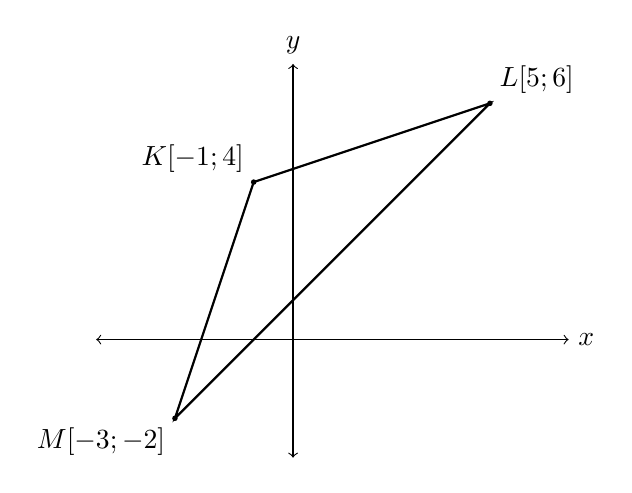
\begin{tikzpicture}[scale=0.5]

            % Body trojúhelníku
            \coordinate (K) at (-1,4);
            \coordinate (L) at (5,6);
            \coordinate (M) at (-3,-2);

            % Osy x a y
            \draw[<->] (-5,0) -- (7,0) node[right] {$x$};
            \draw[<->] (0,-3) -- (0,7) node[above] {$y$};

            % Trojúhelník
            \draw[thick] (K) -- (L) -- (M) -- cycle;

            % Body K, L, M
            \fill (K) circle (2pt) node[above left] {$K[-1;4]$};
            \fill (L) circle (2pt) node[above right] {$L[5;6]$};
            \fill (M) circle (2pt) node[below left] {$M[-3;-2]$};
        \end{tikzpicture}
        \caption{Trojúhelník $KLM$}
        \label{fig:Parametric_lines_in_triangle}
    \end{figure}

    \begin{enumerate}[label=\alph*), leftmargin=2em]

        \item \textbf{Přímka, na níž leží strana $LM$}

        Přímka obsahující stranu $LM$ prochází body $L[5;6]$ a
        $M[-3;-2]$. Její směrový vektor můžeme určit jako
        \[
            \overrightarrow{LM}
            =
            (-3-5;-2-6)
            =
            (-8;-8).
        \]

        Protože směrový vektor přímky můžeme nahradit jeho libovolným nenulovým násobkem, můžeme použít jednodušší vektor
        \[
            \vec{u}_{LM}=(-1;-1).
        \]

        Přímka prochází například bodem $L[5;6]$, a proto její
        parametrické vyjádření je
        \begin{align*}
            p_{LM}: x &= 5-t,\\
                    y &= 6-t;
                    \quad t\in\mathbb{R}.
        \end{align*}

        Správnost můžeme ověřit zjištěním, zda bod $M[-3;-2]$ leží na přímce $p_{LM}$.
        Dosazením do parametrického vyjádření získáme
        \begin{align*}
            -3 &= 5-t,\\
            -2 &= 6-t.
        \end{align*}
        Po upravení obou rovnic dostáváme
        \begin{align*}
            t &= 5+3=8,\\
            t &= 6+2=8.
        \end{align*}
        Odtud $t=8$, což potvrzuje, že bod $M$ leží na přímce $p_{LM}$.
        Přímka $p_{LM}$ obsahující stranu $LM$ je znázorněna na obrázku \ref{fig:Triangle_line_LM}.

        \begin{figure}[H]
            \centering
            \begin{tikzpicture}[scale=0.5]
            
                % Body trojúhelníku
                \coordinate (K) at (-1,4);
                \coordinate (L) at (5,6);
                \coordinate (M) at (-3,-2);
            
                % Osy
                \draw[<->] (-5,0) -- (7,0) node[right] {$x$};
                \draw[<->] (0,-4) -- (0,8) node[above] {$y$};
            
                % Trojúhelník
                \draw[thin,dashed] (K) -- (L) -- (M) -- cycle;
            
                % Přímka obsahující stranu LM
                \draw[thick] (-5,-4) -- (7,8)
                    node[right] {$p_{LM}$};
            
                % Směrový vektor
                \draw[vector] (L) -- ($(L)!0.4!(M)$)
                    node[midway, below left, sloped] {$\vec{u}_{LM}$};
            
                % Body
                \fill (K) circle (2pt) node[above left] {$K$};
                \fill (L) circle (2pt) node[above left] {$L$};
                \fill (M) circle (2pt) node[below right] {$M$};
            
            \end{tikzpicture}
            \caption{Přímka $p_{LM}$, na níž leží strana $LM$ trojúhelníku $KLM$.}
            \label{fig:Triangle_line_LM}
        \end{figure}

        \item \textbf{Výška $v_m$ vedená z vrcholu $M$}

        Výška $v_m$ prochází vrcholem $M$ a je kolmá ke straně $KL$.
        Nejprve proto určíme směrový vektor přímky obsahující stranu
        $KL$:
        \[
            \overrightarrow{KL}
            =
            (5-(-1);6-4)
            =
            (6;2).
        \]

        Tento vektor můžeme zjednodušit na
        \[
            \vec{u}_{KL}=(3;1).
        \]

        Směrový vektor výšky musí být k vektoru $\vec{u}_{KL}$ kolmý, využijeme vlastnost kolmosti vektorů (viz větu o kolmosti vektorů \ref{def:Fast_orthogonal_vector}).
        Zvolíme například
        \[
            \vec{u}_{v_m}=(1;-3),
        \]

        Výška $v_m$ prochází bodem $M[-3;-2]$ a má směrový vektor $\vec{u}_{v_m}$, a proto její parametrické
        vyjádření je
        \begin{align*}
            v_m: x &= -3+t,\\
                 y &= -2-3t;
                 \quad t\in\mathbb{R}.
        \end{align*}

        Výška $v_m$ vedená z vrcholu $M$ kolmo k přímce obsahující stranu $KL$ je znázorněna na obrázku \ref{fig:Triangle_altitude_vm}.

        \begin{figure}[H]
            \centering
            \begin{tikzpicture}[scale=0.5]
            
                % Body trojúhelníku
                \coordinate (K) at (-1,4);
                \coordinate (L) at (5,6);
                \coordinate (M) at (-3,-2);
            
                % Pata výšky na přímce KL
                \coordinate (P) at (-4.6,2.8);
            
                % Osy
                \draw[<->] (-6,0) -- (7,0) node[right] {$x$};
                \draw[<->] (0,-5) -- (0,8) node[above] {$y$};
            
                % Trojúhelník
                \draw[thin,dashed] (K) -- (L) -- (M) -- cycle;
            
                % Přímka obsahující stranu KL
                \draw[thin] (-6,2.33) -- (7,6.67);
            
                % Výška vm
                \draw[very thick] (-5.5,5.5) -- (-1.5,-6.5)
                    node[right] {$v_m$};
            
                % Pravý úhel
                \draw
                    ($(P)+(0.267,0.083)$)
                    --
                    ($(P)+(0.183,0.333)$)
                    --
                    ($(P)+(-0.1,0.25)$);
            
                % Body
                \fill (K) circle (2pt) node[above left] {$K$};
                \fill (L) circle (2pt) node[above right] {$L$};
                \fill (M) circle (2pt) node[below right] {$M$};
                \fill (P) circle (1.5pt) node[above left] {$P$};
            
            \end{tikzpicture}
            \caption{Výška $v_m$ prochází vrcholem $M$ a je kolmá k přímce obsahující stranu $KL$.}
            \label{fig:Triangle_altitude_vm}
        \end{figure}

        \item \textbf{Osa strany $KL$}

        Osa strany $KL$ prochází jejím středem a je ke straně $KL$ kolmá. Nejprve určíme střed strany:
        \begin{align*}
            S_{KL}
            &=
            \left[
                \frac{-1+5}{2};
                \frac{4+6}{2}
            \right]
            =
            [2;5].
        \end{align*}

        Protože osa strany $KL$ je ke straně $KL$ kolmá, můžeme jako
        její směrový vektor použít stejný vektor jako u výšky $v_m$:
        \[
            \vec{u}_{o_{KL}} = \vec{u}_{v_m} = (1;-3).
        \]

        Parametrické vyjádření osy strany $KL$ je tedy
        \begin{align*}
            o_{KL}: x &= 2+t,\\
                    y &= 5-3t;
                    \quad t\in\mathbb{R}.
        \end{align*}

        Výška $v_m$ a osa strany $KL$ mají stejné směrové vektory,
        a jsou proto navzájem rovnoběžné, což odpovídá skutečnosti,
        že obě přímky jsou kolmé ke straně $KL$.

        Osa strany $KL$ je znázorněna na obrázku \ref{fig:Triangle_perpendicular_bisector_KL}. 
        Prochází středem $S_{KL}$ a je ke straně $KL$ kolmá.

        \begin{figure}[H]
            \centering
            \begin{tikzpicture}[scale=0.5]

                % Body trojúhelníku
                \coordinate (K) at (-1,4);
                \coordinate (L) at (5,6);
                \coordinate (M) at (-3,-2);
                \coordinate (Skl) at (2,5);

                % Osy
                \draw[<->] (-5,0) -- (7,0) node[right] {$x$};
                \draw[<->] (0,-4) -- (0,9) node[above] {$y$};

                % Trojúhelník
                \draw[thin,dashed] (K) -- (L) -- (M) -- cycle;

                % Zvýraznění strany KL
                \draw[thin] (K) -- (L);

                % Osa strany KL
                \draw[very thick] (0.5,9.5) -- (4.5,-2.5)
                    node[below right] {$o_{KL}$};

                % Pravý úhel ve středu strany
                \draw
                        ($(Skl)+(0.267,0.083)$)
                        --
                        ($(Skl)+(0.183,0.333)$)
                        --
                        ($(Skl)+(-0.1,0.25)$);

                % Body
                \fill (K) circle (2pt) node[above left] {$K$};
                \fill (L) circle (2pt) node[above right] {$L$};
                \fill (M) circle (2pt) node[below left] {$M$};
                \fill (Skl) circle (2pt) node[above left] {$S_{KL}$};

            \end{tikzpicture}
            \caption{Osa strany $KL$ prochází jejím středem $S_{KL}$ a je ke straně $KL$ kolmá.}
            \label{fig:Triangle_perpendicular_bisector_KL}
        \end{figure}

        \item \textbf{Těžnice $t_L$ vedená z vrcholu $L$}

        Těžnice $t_L$ spojuje vrchol $L$ se středem protější strany
        $KM$. Nejprve proto určíme střed strany $KM$:
        \begin{align*}
            S_{KM}
            &=
            \left[
                \frac{-1+(-3)}{2};
                \frac{4+(-2)}{2}
            \right]
            =
            [-2;1].
        \end{align*}

        Směrový vektor těžnice získáme jako vektor směřující z bodu
        $L$ do bodu $S_{KM}$:
        \[
            \overrightarrow{LS_{KM}}
            =
            (-2-5;1-6)
            =
            (-7;-5).
        \]

        Těžnice prochází bodem $L[5;6]$, a proto její parametrické
        vyjádření je
        \begin{align*}
            t_L: x &= 5-7t,\\
                 y &= 6-5t;
                 \quad t\in\mathbb{R}.
        \end{align*}

        Těžnice $t_l$ spojující vrchol $L$ se středem $S_{KM}$ protější strany je znázorněna na obrázku \ref{fig:Triangle_median_tl}.

        \begin{figure}[H]
            \centering
            \begin{tikzpicture}[scale=0.5]
            
                % Body trojúhelníku
                \coordinate (K) at (-1,4);
                \coordinate (L) at (5,6);
                \coordinate (M) at (-3,-2);
                \coordinate (Skm) at (-2,1);
            
                % Osy
                \draw[<->] (-5,0) -- (7,0) node[right] {$x$};
                \draw[<->] (0,-4) -- (0,8) node[above] {$y$};
            
                % Trojúhelník
                \draw[thin,dashed] (K) -- (L) -- (M) -- cycle;
            
                % Těžnice
                \draw[thin] (6.4,7) -- (-4.8,-1)
                    node[below left] {$t_l$};
            
                % Zvýraznění úseku od L do středu
                \draw[very thick] (L) -- (Skm);
            
                % Body
                \fill (K) circle (2pt) node[above left] {$K$};
                \fill (L) circle (2pt) node[right] {$L$};
                \fill (M) circle (2pt) node[below left] {$M$};
                \fill (Skm) circle (2pt) node[above left] {$S_{KM}$};
            
            \end{tikzpicture}
            \caption{Těžnice $t_l$ vedená z vrcholu $L$ do středu $S_{KM}$ protější strany.}
            \label{fig:Triangle_median_tl}
        \end{figure}

        \item \textbf{Střední příčka $S_{KL}S_{KM}$}

        Střední příčka spojuje středy dvou stran trojúhelníku.
        V předchozích částech jsme určili
        \[
            S_{KL}=[2;5],
            \qquad
            S_{KM}=[-2;1].
        \]

        Směrový vektor přímky obsahující střední příčku je
        \[
            \overrightarrow{S_{KL}S_{KM}}
            =
            (-2-2;1-5)
            =
            (-4;-4).
        \]

        Tento vektor můžeme nahradit jednodušším směrovým vektorem
        \[
            \vec{u}_s=(-1;-1).
        \]

        Parametrické vyjádření přímky obsahující střední příčku je
        proto
        \begin{align*}
            s: x &= 2-t,\\
               y &= 5-t;
               \quad t\in\mathbb{R}.
        \end{align*}

        Směrový vektor střední příčky je rovnoběžný se směrovým
        vektorem strany $LM$, protože
        \[
            \overrightarrow{LM}=(-8;-8)
            =
            8(-1;-1).
        \]
        Tím se potvrzuje známá vlastnost střední příčky trojúhelníku:
        \[
            S_{KL}S_{KM}\parallel LM.
        \]

        Střední příčka $S_{KL}S_{KM}$ je znázorněna na obrázku \ref{fig:Triangle_midline}.
        Z obrázku je patrné, že je rovnoběžná se stranou $LM$.

        \begin{figure}[H]
            \centering
            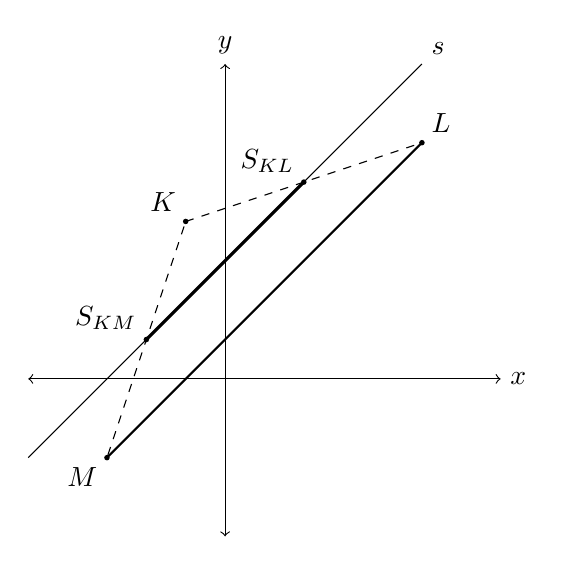
\begin{tikzpicture}[scale=0.5]
            
                % Body trojúhelníku
                \coordinate (K) at (-1,4);
                \coordinate (L) at (5,6);
                \coordinate (M) at (-3,-2);
                \coordinate (Skl) at (2,5);
                \coordinate (Skm) at (-2,1);
            
                % Osy
                \draw[<->] (-5,0) -- (7,0) node[right] {$x$};
                \draw[<->] (0,-4) -- (0,8) node[above] {$y$};
            
                % Trojúhelník
                \draw[thin,dashed] (K) -- (L) -- (M) -- cycle;
            
                % Strana LM
                \draw[thick] (L) -- (M);
            
                % Přímka obsahující střední příčku
                \draw[thin] (-5,-2) -- (5,8)
                    node[above right] {$s$};
            
                % Střední příčka
                \draw[very thick] (Skl) -- (Skm);
            
                % Body
                \fill (K) circle (2pt) node[above left] {$K$};
                \fill (L) circle (2pt) node[above right] {$L$};
                \fill (M) circle (2pt) node[below left] {$M$};
                \fill (Skl) circle (2pt) node[above left] {$S_{KL}$};
                \fill (Skm) circle (2pt) node[above left] {$S_{KM}$};
            
            \end{tikzpicture}
            \caption{Střední příčka $S_{KL}S_{KM}$ je rovnoběžná se stranou $LM$.}
            \label{fig:Triangle_midline}
        \end{figure}
    \end{enumerate}
\end{example}

\subsection{Obecná rovnice přímky}
\label{subsec:General_line_equation}

V předchozí části jsme přímku popisovali pomocí jednoho jejího bodu,
směrového vektoru a parametru. Změnou parametru jsme postupně získávali
jednotlivé body přímky. Parametrické vyjádření nám tedy říká,
\emph{jak body přímky vytvářet}.

Přímku však můžeme popsat také jiným způsobem: jedinou rovnicí o dvou
proměnných $x$ a $y$, kterou splňují právě souřadnice bodů ležících na
přímce. Taková rovnice nám neříká, jak se po přímce pohybovat, ale
umožňuje snadno rozhodnout, zda daný bod na přímce leží. Tento způsob
popisu nazýváme \textbf{obecnou rovnicí přímky}.

Základní roli při jejím odvození bude hrát vektor kolmý k přímce.

\subsubsection{Normálový vektor přímky}
\label{subsubsec:Normal_vector_line}

Při parametrickém vyjádření jsme směr přímky určovali pomocí směrového
vektoru, který je s přímkou rovnoběžný. Nyní budeme pracovat také
s vektorem, který je ke směru přímky kolmý.

\begin{definition}\label{def:Normal_vector_line}
    \textbf{Normálovým vektorem přímky} $p$ nazýváme každý nenulový
    vektor $\vec{n}$, který je kolmý ke směrovému vektoru této přímky,
    a tedy také k přímce samotné.
\end{definition}

Je-li $\vec{u}$ směrovým vektorem přímky $p$ a $\vec{n}$ jejím
normálovým vektorem, platí
\begin{equation}\label{eq:Direction_normal_dot_product}
    \vec{u}\cdot\vec{n}=0.
\end{equation}

Má-li směrový vektor souřadnice
\[
    \vec{u}=(u_x;u_y),
\]
můžeme podle definice~\ref{def:Fast_orthogonal_vector} zvolit například
normálový vektor
\[
    \vec{n}=(u_y;-u_x)
\]
nebo opačně orientovaný vektor
\[
    \vec{n}=(-u_y;u_x).
\]

Naopak známe-li normálový vektor
\[
    \vec{n}=(a;b),
\]
můžeme jako směrový vektor přímky zvolit například
\begin{equation}\label{eq:Direction_vector_from_normal_vector}
    \vec{u}=(-b;a)
\end{equation}
nebo opačně orientovaný vektor
\[
    \vec{u}=(b;-a).
\]
Skutečně platí
\[
    (a;b)\cdot(-b;a)=-ab+ab=0.
\]

Stejně jako směrový vektor ani normálový vektor není určen jednoznačně.
Je-li $\vec{n}$ normálovým vektorem přímky, potom je jejím normálovým
vektorem také každý jeho nenulový reálný násobek
\[
    k\vec{n},
    \qquad
    k\in\mathbb{R}\setminus\{0\}.
\]
Všechny tyto vektory jsou navzájem rovnoběžné a jsou kolmé k téže
přímce.

\begin{figure}[H]
    \centering
    \begin{tikzpicture}[scale=1]

        \coordinate (A) at (0,0);
        \coordinate (U) at (3,1.5);
        \coordinate (N) at (-0.75,1.5);

        % Přímka
        \draw[thin] (-2,-1) -- (5,2.5) node[right] {$p$};

        % Bod
        \fill (A) circle (2pt) node[below right] {$A$};

        % Směrový a normálový vektor
        \draw[vector] (A) -- (U)
            node[midway, above, sloped] {$\vec{u}$};
        \draw[vector] (A) -- (N)
            node[midway, left] {$\vec{n}$};

        % Pravý úhel
        \draw
            (0.30,0.15)
            --
            (0.15,0.45)
            --
            (-0.15,0.30);

    \end{tikzpicture}
    \caption{Směrový vektor $\vec{u}$ je rovnoběžný s přímkou $p$,
    zatímco normálový vektor $\vec{n}$ je k přímce kolmý.}
    \label{fig:Normal_vector_line}
\end{figure}

\subsubsection{Odvození obecné rovnice přímky}
\label{subsubsec:Derivation_general_line_equation}

Uvažujme přímku $p$, která prochází bodem
\[
    A[x_A;y_A]
\]
a má normálový vektor
\[
    \vec{n}=(a;b),
\]
kde alespoň jedna ze souřadnic $a$, $b$ je nenulová. Dále zvolme
libovolný bod roviny
\[
    X[x;y].
\]

Vektor směřující z bodu $A$ do bodu $X$ má souřadnice
\[
    \overrightarrow{AX}=(x-x_A;y-y_A).
\]

Bod $X$ leží na přímce $p$ právě tehdy, když je vektor
$\overrightarrow{AX}$ rovnoběžný s přímkou. Proto musí být kolmý
k jejímu normálovému vektoru $\vec{n}$. Pomocí skalárního součinu tuto
podmínku zapíšeme jako
\begin{equation}\label{eq:Point_normal_condition_line}
    \vec{n}\cdot\overrightarrow{AX}=0.
\end{equation}

Po dosazení souřadnic obou vektorů dostáváme
\begin{align*}
    (a;b)\cdot(x-x_A;y-y_A)&=0,\\
    a(x-x_A)+b(y-y_A)&=0.
\end{align*}

Rovnice
\begin{equation}\label{eq:Point_normal_line_equation}
    a(x-x_A)+b(y-y_A)=0
\end{equation}
popisuje přímku, která prochází bodem $A[x_A;y_A]$ a má normálový
vektor $\vec{n}=(a;b)$.

\begin{figure}[H]
    \centering
    \begin{tikzpicture}[scale=1]

        \coordinate (A) at (0,0);
        \coordinate (X) at (3,1.5);
        \coordinate (Y) at (2.5,2.6);
        \coordinate (N) at (-0.75,1.5);

        % Přímka
        \draw[thin] (-2,-1) -- (5,2.5) node[right] {$p$};

        % Body
        \fill (A) circle (2pt) node[below right] {$A[x_A;y_A]$};
        \fill (X) circle (2pt) node[below right] {$X[x;y]$};
        \fill (Y) circle (2pt) node[above right] {$Y$};

        % Vektory
        \draw[vector] (A) -- (X)
            node[midway, below, sloped] {$\overrightarrow{AX}$};
        \draw[vector] (A) -- (N)
            node[midway, left] {$\vec{n}=(a;b)$};
        \draw[vector, dashed] (A) -- (Y)
            node[midway, above, sloped] {$\overrightarrow{AY}$};

        % Pravý úhel
        \draw
            (0.30,0.15)
            --
            (0.15,0.45)
            --
            (-0.15,0.30);

    \end{tikzpicture}
    \caption{Bod $X$ leží na přímce $p$, protože vektor
    $\overrightarrow{AX}$ je kolmý k normálovému vektoru $\vec{n}$.
    U bodu $Y$, který na přímce neleží, tato kolmost neplatí.}
    \label{fig:General_line_derivation}
\end{figure}

Roznásobením rovnice \eqref{eq:Point_normal_line_equation} získáme
\begin{align*}
    a(x-x_A)+b(y-y_A)&=0,\\
    ax-ax_A+by-by_A&=0,\\
    ax+by-(ax_A+by_A)&=0.
\end{align*}

Bod $A$ i normálový vektor $\vec{n}$ jsou pevně zvolené, a proto je
výraz
\[
    -(ax_A+by_A)
\]
konstantou. Označíme-li tuto konstantu písmenem $c$, dostáváme rovnici
\[
    ax+by+c=0.
\]

\begin{definition}\label{def:General_line_equation}
    \textbf{Obecnou rovnicí přímky} v rovině nazýváme rovnici tvaru
    \begin{equation}\label{eq:General_line_equation}
        ax+by+c=0,
    \end{equation}
    kde
    \[
        a,b,c\in\mathbb{R}
        \qquad\text{a}\qquad
        (a;b)\neq(0;0).
    \]

    Přímka $p$ je množinou všech bodů $X[x;y]$, jejichž souřadnice
    tuto rovnici splňují, tedy
    \[
        X[x;y]\in p
        \quad\Longleftrightarrow\quad
        ax+by+c=0.
    \]
\end{definition}

Podmínka $(a;b)\neq(0;0)$ je nezbytná. Kdyby platilo současně
$a=0$ a $b=0$, rovnice by se zredukovala na vztah
\[
    c=0.
\]
Pro $c=0$ by tuto rovnici splňoval každý bod roviny, zatímco pro
$c\neq0$ by ji nesplňoval žádný bod. Ani v jednom případě by tedy
rovnice nepopisovala přímku.

\begin{remark}\label{rem:Meaning_coefficients_general_line}
    V obecné rovnici $ax + by + c = 0$ jsou čísla $a$, $b$ a $c$ pevnými koeficienty určujícími konkrétní
    přímku. Proměnné $x$ a $y$ představují souřadnice obecného bodu
    roviny.

    Koeficienty $a$ a $b$ současně tvoří souřadnice normálového vektoru
    přímky:
    \begin{equation}\label{eq:Normal_vector_from_general_line}
        \vec{n}=(a;b).
    \end{equation}

    Jako směrový vektor přímky můžeme zvolit například
    \begin{equation}\label{eq:Direction_vector_from_general_line}
        \vec{u}=(-b;a).
    \end{equation}
\end{remark}

\begin{example}\label{exa:Vectors_from_general_line}
    Určete normálový a směrový vektor přímky
    \[
        p: 3x-4y+7=0.
    \]

    Z koeficientů u proměnných $x$ a $y$ přímo získáme normálový
    vektor
    \[
        \vec{n}=(3;-4).
    \]

    Směrový vektor musí být k normálovému vektoru kolmý. 
    Podle definice~\ref{def:Fast_orthogonal_vector} 
    či vztahu \eqref{eq:Direction_vector_from_general_line} můžeme zvolit
    \[
        \vec{u}=(4;3).
    \]

    Kolmost ověříme skalárním součinem:
    \[
        \vec{n}\cdot\vec{u}
        =
        (3;-4)\cdot(4;3)
        =
        12-12
        =
        0.
    \]

    Přímka $p$ má tedy například normálový vektor
    $\vec{n}=(3;-4)$ a směrový vektor $\vec{u}=(4;3)$. Stejně dobře
    bychom mohli zvolit opačný směrový vektor $\vec{u}=(-4;-3)$.
\end{example}

\subsubsection{Nejednoznačnost obecné rovnice}
\label{subsubsec:Nonunique_general_line_equation}

Obecná rovnice přímky, stejně jako její parametrické vyjádření, není
určena jednoznačně. Vynásobením všech členů rovnice stejným nenulovým
číslem se množina jejích řešení nezmění.

Například rovnice
\[
    x-2y+4=0
\]
a
\[
    3x-6y+12=0
\]
popisují tutéž přímku. Druhá rovnice vznikla vynásobením první
rovnice číslem $3$.

Dvě obecné rovnice
\[
    a_1x+b_1y+c_1=0
\]
a
\[
    a_2x+b_2y+c_2=0
\]
určují tutéž přímku právě tehdy, když existuje číslo
$k\in\mathbb{R}\setminus\{0\}$ takové, že
\[
    (a_2;b_2;c_2)=k(a_1;b_1;c_1).
\]

\begin{remark}
    Při zjednodušování obecné rovnice můžeme všechny její koeficienty
    vydělit jejich společným nenulovým dělitelem. Rovnici
    \[
        6x-9y+12=0
    \]
    můžeme například vydělit číslem $3$ a získat jednodušší rovnici
    \[
        2x-3y+4=0.
    \]
    Obě rovnice popisují tutéž přímku.
\end{remark}

\begin{example}\label{exa:Equivalent_general_line_equations}
    Rozhodněte, které z následujících rovnic popisují tutéž přímku:
    \begin{align*}
        p &: 2x-3y+5=0,\\
        q &: -4x+6y-10=0,\\
        r &: 4x-6y+5=0.
    \end{align*}

    Rovnici $q$ můžeme vydělit číslem $-2$ a získáme tak rovnici:
    \[
        -4x+6y-10=0
        \quad\Longrightarrow\quad
        2x-3y+5=0.
    \]
    Rovnice $p$ a $q$ tedy popisují tutéž přímku. Jejich normálové
    vektory jsou proto lineárně závislé a platí
    \begin{align*}
        (2;-3) &= -\frac{1}{2}\cdot(-4;6),\\
        \vec{n}_p &= -\frac{1}{2}\vec{n}_q.
    \end{align*}

    Normálový vektor přímky $r$ je
    \[
        \vec{n}_r=(4;-6)=2\vec{n}_p,
    \]
    takže přímka $r$ má stejný směr jako přímky $p$ a $q$. Trojice
    koeficientů její obecné rovnice však není stejným násobkem trojice
    koeficientů rovnice přímky $p$. Přímka $r$ proto není s přímkami
    $p$ a $q$ totožná, což je patrné také z grafického znázornění
    na obrázku~\ref{fig:Equivalent_general_line_equations}.
    \begin{figure}[H]
        \centering
        \begin{tikzpicture}
            % body
            \coordinate (P_1) at (-4, -1);
            \coordinate (P_2) at (2, 3);
            \coordinate (R_1) at (-2.75, -1);
            \coordinate (R_2) at (3.25, 3);

            % osy x a y
            \draw [<->] (-5,0) -- (5,0) node[right] {$x$};
            \draw [<->] (0,-2) -- (0,4) node[above] {$y$};

            % Jednotky na osách
            \foreach \x in {-4,-3,-2,-1,1,2,3,4} {
                \draw (\x,0.1) -- (\x,-0.1) node[below] {\x};
            }
            \foreach \y in {-1,1,2,3} {
                \draw (0.1,\y) -- (-0.1,\y) node[left] {\y};
            }
            
            % přímky
            \draw[thick, <->] (P_1) -- (P_2) node[above] {$p = q$};
            \draw[thick, <->] (R_1) -- (R_2) node[right] {$r$};
        \end{tikzpicture}
    \caption{Ekvivalentní obecné rovnice přímek.}
    \label{fig:Equivalent_general_line_equations}
    \end{figure}
\end{example}

\subsubsection{Určení obecné rovnice přímky}
\label{subsubsec:Determining_general_line_equation}

Obecná rovnice přímky je určena jejím normálovým vektorem a jedním
bodem, kterým přímka prochází. Podle způsobu zadání proto nejprve
hledáme vhodný normálový vektor a následně použijeme známý bod přímky.

Pro určení obecné rovnice přímky můžeme využít dva základní postupy.
První z nich je založen na dosazování normálového vektoru a bodu do vztahu
\eqref{eq:General_line_equation} a dopočítání konstanty $c$. 
Druhý je založen na dosazování bodu a normálového vektoru do vztahu \eqref{eq:Point_normal_line_equation} a následné úpravě do obecného tvaru.

\begin{example}\label{exa:General_line_from_point_normal}
    Určete obecnou rovnici přímky $p$, která prochází bodem $P[2;-1]$ a má normálový vektor $\vec{n}=(3;2)$.

    Při prvním postupu dosadíme normálový vektor $\vec{n}=(3;2)$ do vztahu
    \eqref{eq:General_line_equation}:
    \begin{align*}
        ax + by + c &= 0,\\
        3x + 2y + c &= 0.
    \end{align*}

    Nyní dopočítáme konstantu $c$ dosazením souřadnic bodu $P[2;-1]$:
    \begin{align*}
        3\cdot2 + 2\cdot(-1) + c &= 0,\\
        6 - 2 + c &= 0,\\
        c &= -4.
    \end{align*}

    Dostáváme obecnou rovnici přímky
    \[
        p: 3x + 2y - 4 = 0.
    \]


    Při druhém postupu dosadíme bod a normálový vektor do vztahu
    \eqref{eq:Point_normal_line_equation}:
    \begin{align*}
        3(x-2)+2(y-(-1))&=0,\\
        3(x-2)+2(y+1)&=0.
    \end{align*}

    Po roznásobení a úpravě dostáváme
    \begin{align*}
        3x-6+2y+2&=0,\\
        3x+2y-4&=0.
    \end{align*}

    Obecná rovnice hledané přímky je tedy
    \[
        p: 3x+2y-4=0.
    \]

    Jak můžeme vidět, obě metody vedou ke stejnému výsledku.
\end{example}

Je-li přímka určena bodem přímky a její směrový vektor, nejprve ke směrovému
vektoru určíme kolmý normálový vektor. Poté postupujeme stejně jako
v předchozím případě.

\begin{example}\label{exa:General_line_from_point_direction}
    Určete obecnou rovnici přímky $q$, která prochází bodem $A[-1;3]$ a má směrový vektor $\vec{u}=(2;-5)$.
    
    K vektoru $\vec{u}=(2;-5)$ zvolíme kolmý normálový vektor
    \[
        \vec{n}=(5;2).
    \]

    Obecnou rovnici přímky nejprve zapíšeme s neurčeným absolutním
    členem $c$:
    \begin{align*}
        ax+by+c &= 0,\\
        5x+2y+c &= 0.
    \end{align*}
    Nyní dopočítáme konstantu $c$ dosazením souřadnic bodu $A[-1;3]$:
    \begin{align*}
        5\cdot(-1) + 2\cdot3 + c &= 0,\\
        -5 + 6 + c &= 0,\\
        c &= -1.
    \end{align*}

    Obecná rovnice hledané přímky je
    \[
        q: 5x+2y-1=0.
    \]
\end{example}

Jsou-li dány dva různé body
\[
    A[x_A;y_A],
    \qquad
    B[x_B;y_B],
\]
je směrovým vektorem přímky vektor
\[
    \overrightarrow{AB}=(x_B-x_A;y_B-y_A).
\]
K němu můžeme zvolit normálový vektor
\[
    \vec{n}=(y_A-y_B;x_B-x_A).
\]
Dosazením bodu $A$ do rovnice určené bodem a normálovým vektorem
získáme
\begin{align*}
    &(y_A-y_B)(x-x_A)+(x_B-x_A)(y-y_A)=0,\\
    &(y_A-y_B)x+(x_B-x_A)y+x_Ay_B-x_By_A=0.
\end{align*}

\begin{example}\label{exa:General_line_from_two_points}
    Určete obecnou rovnici přímky $p_{CD}$, která prochází body
    \[
        C[2;2],
        \qquad
        D[-1;3].
    \]

    Nejprve určíme směrový vektor přímky:
    \[
        \overrightarrow{CD}
        =
        (-1-2;3-2)
        =
        (-3;1).
    \]

    K tomuto vektoru zvolíme kolmý normálový vektor
    \[
        \vec{n}=(1;3).
    \]

    Dosadíme vektor $\vec{n}$ a bod $C[2;2]$ do bodově-normálového tvaru rovnice přímky:
    \begin{align*}
        1(x-2)+3(y-2)&=0,\\
        x-2+3y-6&=0,\\
        x+3y-8&=0.
    \end{align*}
    
    Obecná rovnice přímky $p_{CD}$ je tedy
    \[
        p_{CD}: x+3y-8=0.
    \]

    Výsledek ověříme dosazením druhého bodu $D[-1;3]$:
    \[
        -1+3\cdot3-8=-1+9-8=0.
    \]
\end{example}

\begin{example}\label{exa:Points_on_general_line}
    Rozhodněte, zda body $E[1;2]$ a $F[5;1]$ leží na přímce $p: x+3y-8=0$.

    Pro bod $E[1;2]$ dostáváme
    \[
        1+3\cdot2-8
        =
        -1.
    \]
    Protože výsledek není roven nule, bod $E$ na přímce $p$ tedy neleží.

    Pro bod $F[5;1]$ dostáváme
    \[
        5+3\cdot1-8
        =
        0.
    \]
    Bod $F$ proto na přímce $p$ leží.
\end{example}

\subsubsection{Určování bodů přímky}
\label{subsubsec:Finding_points_general_line}

Obecná rovnice přímky je jedna rovnice o dvou proměnných. Má proto
nekonečně mnoho řešení a každé její řešení představuje jeden bod
přímky. Chceme-li určit konkrétní body, zvolíme vhodnou hodnotu jedné
souřadnice a druhou dopočítáme.

Zvlášť užitečné bývá určit průsečíky přímky se souřadnicovými osami:
\begin{itemize}
    \item bod na ose $x$ má souřadnici $y=0$,
    \item bod na ose $y$ má souřadnici $x=0$.
\end{itemize}

Je-li $a\neq0$, protíná přímka osu $x$ v bodě
\begin{equation}\label{eq:General_line_x_intercept}
    P_x\left[-\frac{c}{a};0\right].
\end{equation}
Je-li $b\neq0$, protíná přímka osu $y$ v bodě
\begin{equation}\label{eq:General_line_y_intercept}
    P_y\left[0;-\frac{c}{b}\right].
\end{equation}

\begin{remark}
    Jestliže $a\neq0$ a $b\neq0$, má přímka
    \[
        ax+by+c=0
    \]
    průsečíky s oběma souřadnicovými osami, a to v bodech
    \[
        P_x\left[-\frac{c}{a};0\right],
        \qquad
        P_y\left[0;-\frac{c}{b}\right].
    \]
\end{remark}

\begin{example}\label{exa:Finding_points_general_line}
    Určete tři body přímky
    \[
        p: 2x+3y-6=0
    \]
    a přímku zakreslete do kartézské soustavy souřadnic.

    Nejprve určíme průsečík s osou $x$. Položíme $y=0$:
    \begin{align*}
        2x+3\cdot0-6&=0,\\
        2x&=6,\\
        x&=3.
    \end{align*}
    Na přímce tedy leží bod
    \[
        A[3;0].
    \]

    Ke stejnému výsledku bychom dospěli také podle vztahu \eqref{eq:General_line_x_intercept}:
    \[
        P_x\left[-\frac{-6}{2};0\right]
        =
        P_x[3;0].
    \]

    Nyní určíme průsečík s osou $y$. Položíme $x=0$:
    \begin{align*}
        2\cdot0+3y-6&=0,\\
        3y&=6,\\
        y&=2.
    \end{align*}
    Na přímce leží také bod
    \[
        B[0;2].
    \]

    Ke stejnému výsledku bychom dospěli také podle vztahu \eqref{eq:General_line_y_intercept}:
    \[
        P_y\left[0;-\frac{-6}{3}\right]
        =
        P_y[0;2].
    \]

    Pro získání třetího bodu zvolíme například $x=-3$:
    \begin{align*}
        2\cdot(-3)+3y-6&=0,\\
        -6+3y-6&=0,\\
        3y&=12,\\
        y&=4.
    \end{align*}
    Třetím bodem je
    \[
        C[-3;4].
    \]

    Všechny tři body skutečně leží na jedné přímce, jak ukazuje
    obrázek \ref{fig:General_line_from_points}.

    \begin{figure}[H]
        \centering
        \begin{tikzpicture}[scale=0.8]

            % Osy
            \draw[<->] (-4.5,0) -- (5,0) node[right] {$x$};
            \draw[<->] (0,-2) -- (0,5) node[above] {$y$};
            \node[below left] at (0,0) {$O$};

            % Přímka
            \draw[thick, <->] (-4.5,5) -- (5,-1.333)
                node[right] {$p$};

            % Body
            \fill (3,0) circle (2.5pt) node[above right] {$P_x = A[3;0]$};
            \fill (0,2) circle (2.5pt) node[above right] {$P_y = B[0;2]$};
            \fill (-3,4) circle (2.5pt) node[above left] {$C[-3;4]$};

        \end{tikzpicture}
        \caption{Tři body přímky $p:2x+3y-6=0$.}
        \label{fig:General_line_from_points}
    \end{figure}
\end{example}

\subsubsection{Zvláštní případy obecné rovnice}
\label{subsubsec:Special_general_line_equations}

Podle toho, které koeficienty obecné rovnice jsou nulové, můžeme snadno
rozpoznat některé zvláštní polohy přímky vůči souřadnicovým osám.

\paragraph{Přímka rovnoběžná s osou $x$.}

Jestliže $a=0$, má rovnice tvar
\[
    by+c=0.
\]
Protože musí platit $b\neq0$, můžeme určit
\[
    y=-\frac{c}{b}.
\]
Souřadnice $y$ je pro všechny body přímky stejná, a proto je přímka
rovnoběžná s osou $x$.

\begin{example}
    Určete geometrický význam rovnice $2y-6=0$.

    Protože koeficient u $x$ je nulový, jde o přímku rovnoběžnou s osou $x$.
    Po úpravě dostáváme
    \[
        y=3.
    \]
    Rovnice tedy popisuje vodorovnou přímku:
    \begin{figure}[H]
         \centering
        \begin{tikzpicture}[scale=0.8]
            % Osy
            \draw[<->] (-1,0) -- (5,0) node[right] {$x$};
            \draw[<->] (0,-1) -- (0,5) node[above] {$y$};
            \node[below left] at (0,0) {$O$};

            % Přímka
            \draw[thick, <->] (-1,3) -- (5,3)
                node[right] {$p:2y-6=0$};

            % Jednotky na osách
            \foreach \x in {1,2,3,4} {
                \draw (\x,0.1) -- (\x,-0.1) node[below] {\x};
            }
            \foreach \y in {1,2,3,4} {
                \draw (0.1,\y) -- (-0.1,\y) node[left] {\y};
            }

            % Body
            \fill (0,3) circle (2.5pt) node[above left] {$P_y[0;3]$};
            \fill (4,3) circle (2.5pt) node[above right] {$Q[4;3]$};
        \end{tikzpicture}
        \caption{Přímka $p:2y-6=0$ je rovnoběžná s osou $x$.}
        \label{fig:Line_parallel_x_axis}
    \end{figure}
\end{example}

\paragraph{Přímka rovnoběžná s osou $y$.}

Jestliže $b=0$, má rovnice tvar
\[
    ax+c=0.
\]
Protože musí platit $a\neq0$, dostáváme
\[
    x=-\frac{c}{a}.
\]
Souřadnice $x$ je pro všechny body přímky stejná, a proto je přímka
rovnoběžná s osou $y$.

\begin{example}
    Určete geometrický význam rovnice $3x+12=0$.

    Protože koeficient u $y$ je nulový, jde o přímku rovnoběžnou s osou $y$.
    Po úpravě dostáváme
    \[
        x=-4.
    \]
    Rovnice tedy popisuje svislou přímku:
    \begin{figure}[H]
         \centering
        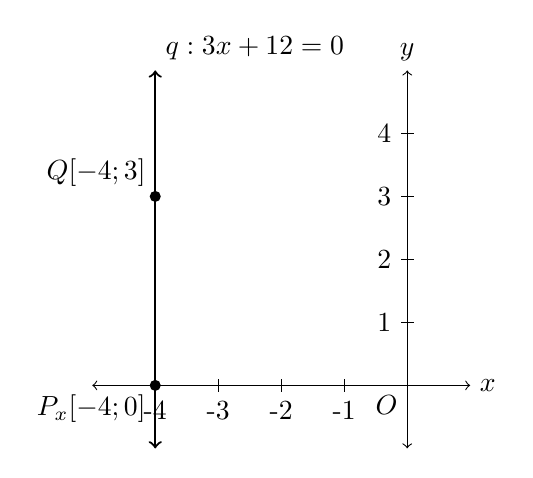
\begin{tikzpicture}[scale=0.8]
            % Osy
            \draw[<->] (-5,0) -- (1,0) node[right] {$x$};
            \draw[<->] (0,-1) -- (0,5) node[above] {$y$};
            \node[below left] at (0,0) {$O$};

            % Přímka
            \draw[thick, <->] (-4,-1) -- (-4,5)
                node[above right] {$q:3x+12=0$};

            % Jednotky na osách
            \foreach \x in {-4,-3,-2,-1} {
                \draw (\x,0.1) -- (\x,-0.1) node[below] {\x};
            }
            \foreach \y in {1,2,3,4} {
                \draw (0.1,\y) -- (-0.1,\y) node[left] {\y};
            }

            % Body
            \fill (-4,0) circle (2.5pt) node[below left] {$P_x[-4;0]$};
            \fill (-4,3) circle (2.5pt) node[above left] {$Q[-4;3]$};
        \end{tikzpicture}
        \caption{Přímka $q:3x+12=0$ je rovnoběžná s osou $y$.}
        \label{fig:Line_parallel_y_axis}
    \end{figure}
\end{example}

\paragraph{Přímka procházející počátkem soustavy souřadnic.}

Jestliže $c=0$, má rovnice tvar
\[
    ax+by=0.
\]
Počátek soustavy souřadnic $O[0;0]$ tuto rovnici vždy splňuje, protože
\[
    a\cdot0+b\cdot0=0.
\]
Každá přímka s nulovým absolutním členem tedy prochází počátkem.

Zvláštními případy jsou také samotné souřadnicové osy:
\[
    x=0
    \qquad\text{je rovnice osy }y,
\]
\[
    y=0
    \qquad\text{je rovnice osy }x.
\]

\begin{example}\label{exa:Special_general_line_equations}
    Určete geometrický význam následujících rovnic:
    \begin{align*}
        p &: 2y-6=0,\\
        q &: 3x+12=0,\\
        r &: 4x-2y=0.
    \end{align*}

    U přímky $p$ je koeficient u $x$ nulový. Po úpravě dostáváme
    \[
        y=3.
    \]
    Jde tedy o vodorovnou přímku rovnoběžnou s osou $x$.

    U přímky $q$ je koeficient u $y$ nulový. Po úpravě dostáváme
    \[
        x=-4.
    \]
    Jde tedy o svislou přímku rovnoběžnou s osou $y$.

    U přímky $r$ je absolutní člen nulový, a proto přímka prochází
    počátkem soustavy souřadnic. Například body
    \[
        O[0;0]
        \qquad\text{a}\qquad
        A[1;2]
    \]
    její rovnici splňují.
\end{example}

\subsubsection{Souhrnný příklad s trojúhelníkem}
\label{subsubsec:General_lines_triangle}

Vrátíme se nyní k trojúhelníku $KLM$ z příkladu~\ref{exa:Parametric_lines_in_triangle}. Tentokrát budeme významné
přímky spojené s trojúhelníkem zapisovat pomocí obecných rovnic.
Příklad tak znovu propojí souřadnice bodů, středy úseček, směrové
a normálové vektory i kolmost přímek.

\begin{example}\label{exa:General_lines_in_triangle}
    Je dán trojúhelník $KLM$ s vrcholy
    \[
        K[-1;4],
        \qquad
        L[5;6],
        \qquad
        M[-3;-2].
    \]
    Trojúhelník je znázorněn na obrázku~\ref{fig:Parametric_lines_in_triangle}.

    Určete obecné rovnice přímek, na nichž leží:
    \begin{enumerate}[label=\alph*)]
        \item strana $LM$,
        \item výška $v_m$ vedená z vrcholu $M$,
        \item osa strany $KL$,
        \item těžnice $t_L$ vedená z vrcholu $L$,
        \item střední příčka spojující středy stran $KL$ a $KM$.
    \end{enumerate}

    Středy stran $KL$ a $KM$ budeme označovat $S_{KL}$ a $S_{KM}$.

    \begin{enumerate}[label=\alph*), leftmargin=2em]

        \item \textbf{Přímka, na níž leží strana $LM$}

        Přímka prochází body $L[5;6]$ a $M[-3;-2]$. Její směrový
        vektor je
        \[
            \overrightarrow{LM}
            =
            (-3-5;-2-6)
            =
            (-8;-8).
        \]

        Použijeme jednodušší směrový vektor
        \[
            \vec{u}_{LM}=(-1;-1).
        \]
        K němu zvolíme normálový vektor
        \[
            \vec{n}_{LM}=(1;-1).
        \]

        Rovnice přímky má tvar
        \[
            x-y+c=0.
        \]
        Dosadíme bod $L[5;6]$:
        \begin{align*}
            5-6+c&=0,\\
            c&=1.
        \end{align*}

        Přímka obsahující stranu $LM$ má rovnici
        \[
            p_{LM}: x-y+1=0.
        \]

        Ověření bodem $M[-3;-2]$:
        \[
            -3-(-2)+1=0.
        \]

        \item \textbf{Výška $v_m$ vedená z vrcholu $M$}

        Výška $v_m$ je kolmá ke straně $KL$. Směrový vektor strany
        $KL$ je
        \[
            \overrightarrow{KL}
            =
            (5-(-1);6-4)
            =
            (6;2).
        \]
        Použijeme jednodušší vektor
        \[
            \vec{u}_{KL}=(3;1).
        \]

        Protože je výška $v_m$ ke straně $KL$ kolmá, může být vektor
        $\vec{u}_{KL}$ normálovým vektorem výšky:
        \[
            \vec{n}_{v_m}=(3;1).
        \]

        Rovnice výšky má tvar
        \[
            3x+y+c=0.
        \]
        Dosadíme vrchol $M[-3;-2]$:
        \begin{align*}
            3\cdot(-3)+(-2)+c&=0,\\
            -11+c&=0,\\
            c&=11.
        \end{align*}

        Výška $v_m$ má rovnici
        \[
            v_m: 3x+y+11=0.
        \]

        \item \textbf{Osa strany $KL$}

        Osa strany $KL$ prochází jejím středem a je ke straně $KL$
        kolmá. Nejprve určíme střed strany:
        \begin{align*}
            S_{KL}
            &=
            \left[
                \frac{-1+5}{2};
                \frac{4+6}{2}
            \right] = [2;5].
        \end{align*}

        Osa strany $KL$ je stejně jako výška $v_m$ kolmá ke straně
        $KL$, a proto můžeme použít stejný normálový vektor
        \[
            \vec{n}_{o_{KL}}=(3;1).
        \]

        Rovnice osy má tvar
        \[
            3x+y+c=0.
        \]
        Dosadíme bod $S_{KL}[2;5]$:
        \begin{align*}
            3\cdot2+5+c&=0,\\
            11+c&=0,\\
            c&=-11.
        \end{align*}

        Osa strany $KL$ má rovnici
        \[
            o_{KL}: 3x+y-11=0.
        \]

        Výška $v_m$ a osa strany $KL$ mají rovnoběžné normálové
        vektory, ale různé absolutní členy. Jsou tedy navzájem
        rovnoběžné.

        \item \textbf{Těžnice $t_L$ vedená z vrcholu $L$}

        Těžnice $t_L$ spojuje vrchol $L$ se středem protější strany
        $KM$. Nejprve určíme tento střed:
        \begin{align*}
            S_{KM}
            &=
            \left[
                \frac{-1+(-3)}{2};
                \frac{4+(-2)}{2}
            \right] = [-2;1].
        \end{align*}

        Směrový vektor těžnice je
        \[
            \overrightarrow{LS_{KM}}
            =
            (-2-5;1-6)
            =
            (-7;-5).
        \]
        K tomuto směrovému vektoru zvolíme normálový vektor
        \[
            \vec{n}_{t_L}=(5;-7),
        \]
        protože
        \[
            (-7;-5)\cdot(5;-7)=-35+35=0.
        \]

        Rovnice těžnice má tvar
        \[
            5x-7y+c=0.
        \]
        Dosadíme vrchol $L[5;6]$:
        \begin{align*}
            5\cdot5-7\cdot6+c&=0,\\
            25-42+c&=0,\\
            c&=17.
        \end{align*}

        Těžnice $t_L$ má rovnici
        \[
            t_L: 5x-7y+17=0.
        \]

        \item \textbf{Střední příčka $S_{KL}S_{KM}$}

        Již známe oba středy:
        \[
            S_{KL}[2;5],
            \qquad
            S_{KM}[-2;1].
        \]

        Směrový vektor střední příčky je
        \[
            \overrightarrow{S_{KL}S_{KM}}
            =
            (-2-2;1-5)
            =
            (-4;-4).
        \]
        Použijeme jednodušší směrový vektor
        \[
            \vec{u}_s=(-1;-1)
        \]
        a k němu normálový vektor
        \[
            \vec{n}_s=(1;-1).
        \]

        Rovnice přímky obsahující střední příčku má tvar
        \[
            x-y+c=0.
        \]
        Dosadíme bod $S_{KL}[2;5]$:
        \begin{align*}
            2-5+c&=0,\\
            c&=3.
        \end{align*}

        Přímka obsahující střední příčku má rovnici
        \[
            s: x-y+3=0.
        \]

        Přímky
        \[
            p_{LM}:x-y+1=0
        \]
        a
        \[
            s:x-y+3=0
        \]
        mají stejné koeficienty u proměnných $x$ a $y$, ale různé
        absolutní členy. Jsou tedy rovnoběžné, čímž se opět potvrzuje známá
        vlastnost střední příčky trojúhelníku:
        \[
            S_{KL}S_{KM}\parallel LM.
        \]

    \end{enumerate}
\end{example}

\begin{example}\label{exa:Central_symmetry_line}
    Je dána přímka
    \[
        p:2x-y+1=0.
    \]
    Určete rovnici přímky $p'$, která je obrazem přímky $p$ ve
    středové souměrnosti se středem
    \[
        S[-2;1].
    \]

    Situace je znázorněnáo na obrázku \ref{fig:Central_symmetry_line}.
    
    Přímku $p'$ můžeme určit pomocí obrazů dvou různých bodů přímky
    $p$. Pro obraz libovolného bodu $X$ ve středové souměrnosti se
    středem $S$ platí
    \[
        X'=S+(S-X)=2S-X.
    \]

    Nejprve tedy na přímce $p$ zvolíme dva různé body, určíme jejich
    obrazy a následně sestavíme rovnici přímky procházející těmito
    obrazy.

    Zvolíme nejprve bod s první souřadnicí $x=0$. Dosadíme do rovnice
    přímky $p$:
    \begin{align*}
        2\cdot0-y+1&=0,\\
        -y+1&=0,\\
        y&=1.
    \end{align*}

    Na přímce $p$ tedy leží bod
    \[
        A[0;1].
    \]

    Jako druhý bod zvolíme bod s první souřadnicí $x=1$:
    \begin{align*}
        2\cdot1-y+1&=0,\\
        3-y&=0,\\
        y&=3.
    \end{align*}

    Druhým bodem přímky $p$ je
    \[
        B[1;3].
    \]

    Nyní určíme obraz bodu $A$ ve středové souměrnosti se středem
    $S[-2;1]$:
    \begin{align*}
        A'
        &=
        S+(S-A)\\
        &=
        [-2;1]+\bigl([-2;1]-[0;1]\bigr)\\
        &=
        [-2;1]+(-2;0)\\
        &=
        [-4;1].
    \end{align*}

    Obdobně určíme obraz bodu $B$:
    \begin{align*}
        B'
        &=
        S+(S-B)\\
        &=
        [-2;1]+\bigl([-2;1]-[1;3]\bigr)\\
        &=
        [-2;1]+(-3;-2)\\
        &=
        [-5;-1].
    \end{align*}

    Obrazem přímky $p$ je přímka $p'$, která prochází body
    \[
        A'[-4;1]
        \qquad\text{a}\qquad
        B'[-5;-1].
    \]

    Její směrový vektor můžeme určit jako
    \[
        \overrightarrow{A'B'}
        =
        (-5-(-4);-1-1)
        =
        (-1;-2).
    \]

    K tomuto směrovému vektoru zvolíme normálový vektor
    \[
        \vec{n}_{p'}=(2;-1),
    \]
    protože
    \[
        (-1;-2)\cdot(2;-1)
        =
        -2+2
        =
        0.
    \]

    Obecná rovnice přímky $p'$ má tedy tvar
    \[
        2x-y+c=0.
    \]

    Dosadíme například bod $A'[-4;1]$:
    \begin{align*}
        2\cdot(-4)-1+c&=0,\\
        -8-1+c&=0,\\
        c&=9.
    \end{align*}

    Hledaná přímka má rovnici
    \[
        p':2x-y+9=0.
    \]

    Přímky $p$ a $p'$ mají stejné normálové vektory, a jsou proto
    rovnoběžné. To odpovídá vlastnosti středové souměrnosti: obrazem
    přímky, která neprochází středem souměrnosti, je přímka s ní
    rovnoběžná.

    \begin{figure}[H]
        \centering
        \begin{tikzpicture}[scale=0.9]

            % Přímky
            \draw[thin, <->]
                (-1.5,-2) -- (2.5,6)
                node[above right] {$p$};

            \draw[thin, <->]
                (-5.5,-2) -- (-1.5,6)
                node[above right] {$p'$};

            % Body
            \coordinate (A) at (0,1);
            \coordinate (B) at (1,3);
            \coordinate (S) at (-2,1);
            \coordinate (Ap) at (-4,1);
            \coordinate (Bp) at (-5,-1);

            \fill (A) circle (2.5pt)
                node[below right] {$A$};
            \fill (B) circle (2.5pt)
                node[below right] {$B$};
            \fill (S) circle (2.5pt)
                node[above right] {$S$};
            \fill (Ap) circle (2.5pt)
                node[above left] {$A'$};
            \fill (Bp) circle (2.5pt)
                node[below left] {$B'$};

            % Spojnice bodů se středem
            \draw[vector] (A) -- (S);
            \draw[vector] (S) -- (Ap);

            \draw[vector] (B) -- (S);
            \draw[vector] (S) -- (Bp);

        \end{tikzpicture}
        \caption{Přímka $p'$ je obrazem přímky $p$ ve středové
        souměrnosti se středem $S$.}
        \label{fig:Central_symmetry_line}
    \end{figure}
\end{example}
\subsection{Směrnicový tvar rovnice přímky}
\label{subsec:Slope_intercept_line_equation}

V předchozích částech jsme přímku popisovali pomocí parametrického
vyjádření a obecné rovnice. Přímka však může být zároveň grafem funkce.
Z předchozího studia funkcí víme, že grafem lineární funkce
\[
    f(x)=ax+b
\]
je přímka.

Zapíšeme-li funkční předpis ve tvaru
\[
    y=kx+q,
\]
můžeme jej chápat nejen jako předpis funkce, ale také jako rovnici
přímky. Proměnná $x$ představuje první souřadnici bodu přímky
a hodnota $y$ jeho druhou souřadnici.

Tento způsob zápisu má jednu důležitou vlastnost. Každé hodnotě
$x\in\mathbb{R}$ je přiřazena právě jedna hodnota $y$. Přímka zapsaná
tímto způsobem proto nesmí být rovnoběžná s osou $y$, protože na svislé
přímce se může pro jednu hodnotu $x$ nacházet nekonečně mnoho bodů
s různými souřadnicemi $y$.

\begin{definition}\label{def:Slope_intercept_line_equation}
    Nechť $k,q\in\mathbb{R}$. Rovnici
    \begin{equation}\label{eq:Slope_intercept_line_equation}
        y=kx+q
    \end{equation}
    nazýváme \textbf{směrnicovým tvarem rovnice přímky}.

    Číslo $k$ nazýváme \textbf{směrnicí přímky} a číslo $q$
    \textbf{úsekem přímky na ose $y$}.
\end{definition}

Směrnicovým tvarem lze popsat každou přímku, která není rovnoběžná
s osou $y$. Pro takovou přímku jsou čísla $k$ a $q$ určena jednoznačně.
To znamená, že dva různé směrnicové tvary nemohou popisovat tutéž
přímku.

Svislé přímky mají rovnice tvaru
\[
    x=d,
    \qquad d\in\mathbb{R},
\]
a ve směrnicovém tvaru je zapsat nelze.

\subsubsection{Význam koeficientů $k$ a $q$}
\label{subsubsec:Meaning_slope_intercept_coefficients}

V rovnici
\[
    y=kx+q
\]
mají oba koeficienty přímý geometrický význam.

Dosadíme-li $x=0$, získáme
\[
    y=k\cdot0+q=q.
\]
Přímka proto vždy prochází bodem
\begin{equation}\label{eq:Y_intercept_point}
    Q[0;q].
\end{equation}

Číslo $q$ tedy určuje průsečík přímky s osou $y$. Změníme-li pouze
hodnotu $q$ a směrnici $k$ ponecháme stejnou, posuneme přímku ve
svislém směru, ale její směr se nezmění. Všechny přímky se stejnou
směrnicí jsou proto navzájem rovnoběžné nebo totožné.

Směrnice $k$ určuje, jak se změní souřadnice $y$, zvětšíme-li
souřadnici $x$ o jednu jednotku. Jestliže bod
\[
    A[x_A;y_A]
\]
leží na přímce, potom bod s první souřadnicí $x_A+1$ má druhou
souřadnici
\[
    y_A+k.
\]

Směrnice tedy vyjadřuje změnu druhé souřadnice připadající na jednotkovou
změnu první souřadnice.

\begin{figure}[H]
    \centering
    \begin{tikzpicture}[scale=1]

        % Osy
        \draw[<->] (-2,0) -- (5.5,0)
            node[right] {$x$};

        \draw[<->] (0,-0.8) -- (0,4.7)
            node[above] {$y$};

        \node[below left] at (0,0) {$O$};

        % Přímka y = kx + q
        \draw[thick, <->]
            (-1.5,0.1) -- (5,4)
            node[above right] {$p:y=kx+q$};

        % Body
        \coordinate (Q) at (0,1);
        \coordinate (R) at (2,1);
        \coordinate (A) at (2,2.2);

        \fill (Q) circle (2pt)
            node[left] {$Q[0;q]$};

        \fill (A) circle (2pt);

        % Pomocný pravoúhlý trojúhelník
        \draw[dashed] (Q) -- (R)
            node[midway, below] {$1$};

        \draw[dashed] (R) -- (A)
            node[midway, right] {$k$};

        % Úhel phi
        \draw (0.65,1)
            arc[start angle=0,end angle=31,radius=0.65];

        \node at (0.82,1.23) {$\varphi$};

        % Hodnota q na ose y
        \draw (-0.08,1) -- (0.08,1);
        \node[right] at (0,0.72) {$q$};

    \end{tikzpicture}

    \caption{Geometrický význam koeficientů $k$ a $q$
    ve směrnicovém tvaru přímky.}
    \label{fig:Slope_intercept_coefficients}
\end{figure}

Podle hodnoty směrnice mohou nastat následující případy:
\begin{itemize}
    \item je-li $k>0$, přímka je rostoucí;
    \item je-li $k<0$, přímka je klesající;
    \item je-li $k=0$, přímka je rovnoběžná s osou $x$.
\end{itemize}

\begin{remark}\label{rem:Special_slope_intercept_coefficients}
    Jestliže $q=0$, má přímka rovnici $y=kx$ a prochází počátkem soustavy souřadnic $O[0;0]$.

    Jestliže současně $k=0$, dostáváme rovnici
    \[
        y=0,
    \]
    která popisuje osu $x$.
\end{remark}

\subsubsection{Směrnice určená dvěma body}
\label{subsubsec:Slope_from_two_points}

Uvažujme dva různé body
\[
    A[x_A;y_A],
    \qquad
    B[x_B;y_B],
\]
které leží na přímce
\[
    y=kx+q.
\]

Pro jejich souřadnice platí
\[
    y_A=kx_A+q
\]
a
\[
    y_B=kx_B+q.
\]

Odečtením první rovnice od druhé získáme
\begin{align*}
    y_B-y_A &= kx_B+q-(kx_A+q),\\
    y_B-y_A &= kx_B-kx_A+q-q, \\
    y_B-y_A &= k(x_B-x_A).
\end{align*}

Jestliže $x_A\neq x_B$, můžeme rovnici vydělit rozdílem
$x_B-x_A$ a dostáváme
\begin{equation}\label{eq:Slope_from_two_points}
    k=
    \frac{y_B-y_A}{x_B-x_A}.
\end{equation}

Směrnici tedy můžeme chápat jako poměr změny souřadnice $y$ ke změně
souřadnice $x$:
\[
    k=\frac{\Delta y}{\Delta x}.
\]

Rozdíl
\[
    \Delta x=x_B-x_A
\]
představuje vodorovnou změnu mezi body, zatímco
\[
    \Delta y=y_B-y_A
\]
představuje změnu svislou.

Pokud platí $x_A=x_B$, je jmenovatel ve vztahu
\eqref{eq:Slope_from_two_points} nulový. Body $A$ a $B$ potom leží na
svislé přímce, jejíž směrnice není definována.

\begin{example}\label{exa:Slope_from_two_points}
    Určete směrnici přímky procházející body
    \[
        A[-2;1],
        \qquad
        B[4;4].
    \]

    Použijeme vztah \eqref{eq:Slope_from_two_points}:
    \[
        k
        =
        \frac{4-1}{4-(-2)}
        =
        \frac{3}{6}
        =
        \frac{1}{2}.
    \]

    Směrnice přímky je tedy
    \[
        k=\frac{1}{2}.
    \]

    To znamená, že při zvětšení souřadnice $x$ o dvě jednotky se
    souřadnice $y$ zvětší o jednu jednotku.
\end{example}

\subsubsection{Směrový úhel přímky a funkce tangens}
\label{subsubsec:Slope_angle_tangent}

Směrnici přímky můžeme vyjádřit také pomocí goniometrických funkcí.
Uvažujme přímku, která není rovnoběžná s osou $y$, a označme
$\varphi$ její \textbf{směrový úhel}, tedy úhel, který přímka svírá
s kladnou poloosou $x$.

Směrový úhel volíme z intervalu
\[
    \varphi\in\langle 0^\circ;180^\circ),
\]
přičemž pro nesvislou přímku platí
\[
    \varphi\neq90^\circ.
\]

Z pravoúhlého trojúhelníku na obrázku
\ref{fig:Slope_intercept_coefficients} získáme
\[
    \tan\varphi
    =
    \frac{\text{změna souřadnice }y}
         {\text{změna souřadnice }x}.
\]

Protože směrnice přímky je právě poměrem těchto změn, platí
\begin{equation}\label{eq:Slope_tangent_relation}
    k=\tan\varphi.
\end{equation}

Tento vztah propojuje analytickou geometrii s goniometrickými funkcemi.
Směrnici můžeme určit ze směrového úhlu a naopak směrový úhel můžeme
určit ze směrnice.

Je-li známá směrnice $k$, hledáme úhel splňující
\[
    \tan\varphi=k.
\]

Pro kladnou směrnici dostáváme ostrý úhel
\[
    0^\circ<\varphi<90^\circ.
\]

Pro zápornou směrnici musí být směrový úhel tupý:
\[
    90^\circ<\varphi<180^\circ.
\]

\begin{remark}\label{rem:Arctangent_negative_slope}
    Kalkulačka vrací při výpočtu $\arctan k$ obvykle hodnotu
    z intervalu
    \[
        (-90^\circ;90^\circ).
    \]
    Pro zápornou směrnici proto dostaneme záporný úhel. Chceme-li
    určit směrový úhel přímky z intervalu
    $\langle0^\circ;180^\circ)$, musíme k této hodnotě přičíst
    $180^\circ$.
\end{remark}

\begin{example}\label{exa:Direction_angle_from_slope}
    Určete směrový úhel přímky se směrnicí $k=-2$.

    Hledáme úhel $\varphi$, pro který platí
    \[
        \tan\varphi=-2.
    \]

    Kalkulačka dává
    \[
        \arctan(-2)\doteq-63^\circ26'.
    \]

    Protože je směrnice záporná, musí být směrový úhel přímky tupý.
    Přičteme tedy $180^\circ$:
    \[
        \varphi
        \doteq
        180^\circ-63^\circ26'
        =
        116^\circ34'.
    \]

    Směrový úhel přímky je přibližně
    \[
        \varphi\doteq116^\circ34'.
    \]
\end{example}

Pro vodorovnou přímku platí
\[
    k=0,
    \qquad
    \varphi=0^\circ.
\]

Svislá přímka má směrový úhel
\[
    \varphi=90^\circ,
\]
ale její směrnice není definována, protože funkce tangens není pro
úhel $90^\circ$ definována.

\subsubsection{Vztah směrnice a směrového vektoru}
\label{subsubsec:Slope_direction_vector}

Směrnice i směrový vektor určují směr přímky, a proto spolu musí
souviset.

Uvažujme přímku
\[
    y=kx+q.
\]
Zvětšíme-li souřadnici $x$ o jednu jednotku, změní se souřadnice $y$
o hodnotu $k$. Po přímce se tedy můžeme posunout o vektor
\begin{equation}\label{eq:Direction_vector_from_slope}
    \vec{u}=(1;k).
\end{equation}

Tento vektor je směrovým vektorem přímky. Stejně jako dříve jej můžeme
nahradit libovolným nenulovým násobkem:
\[
    \vec{u}=t(1;k),
    \qquad
    t\in\mathbb{R}\setminus\{0\}.
\]

Naopak má-li přímka směrový vektor
\[
    \vec{u}=(u_x;u_y),
\]
kde $u_x\neq0$, je její směrnice
\begin{equation}\label{eq:Slope_from_direction_vector}
    k=\frac{u_y}{u_x}.
\end{equation}

Tento vztah opět odpovídá poměru svislé a vodorovné změny.

\begin{example}\label{exa:Slope_from_direction_vector}
    Určete směrnici přímky, jejímž směrovým vektorem je
    \[
        \vec{u}=(-4;6).
    \]

    Podle vztahu \eqref{eq:Slope_from_direction_vector} platí
    \[
        k
        =
        \frac{6}{-4}
        =
        -\frac{3}{2}.
    \]

    Přímka má tedy směrnici
    \[
        k=-\frac{3}{2}.
    \]

    Stejnou směrnici bychom získali také z jednoduššího směrového
    vektoru
    \[
        \vec{v}=(2;-3),
    \]
    který je nenulovým násobkem původního vektoru.
\end{example}

Jestliže $u_x=0$, má směrový vektor tvar
\[
    \vec{u}=(0;u_y).
\]
Takový vektor určuje svislý směr. Přímka je tedy rovnoběžná s osou
$y$ a její směrnice není definována.

\subsubsection{Přímka určená bodem a směrnicí}
\label{subsubsec:Line_from_point_and_slope}

Známe-li směrnici přímky a jeden její bod, můžeme její rovnici snadno
určit.

Uvažujme přímku se směrnicí $k$, která prochází bodem
\[
    A[x_A;y_A].
\]

Směrnicový tvar má podobu
\[
    y=kx+q.
\]
Protože bod $A$ na přímce leží, musí jeho souřadnice rovnici splňovat:
\[
    y_A=kx_A+q.
\]

Odtud vyjádříme
\[
    q=y_A-kx_A.
\]

Dosazením do směrnicového tvaru dostáváme
\begin{align*}
    y
    &=
    kx+y_A-kx_A,\\
    y-y_A
    &=
    kx-kx_A.
\end{align*}

Po vytknutí směrnice $k$ získáme
\begin{equation}\label{eq:Point_slope_line_equation}
    y-y_A=k(x-x_A).
\end{equation}

\begin{definition}\label{def:Point_slope_line_equation}
    Rovnici
    \[
        y-y_A=k(x-x_A)
    \]
    nazýváme \textbf{bodově-směrnicovým tvarem rovnice přímky}.
    Popisuje přímku se směrnicí $k$, která prochází bodem
    $A[x_A;y_A]$.
\end{definition}

Výhodou tohoto zápisu je, že nemusíme nejprve určovat koeficient $q$.
Známý bod a směrnici dosadíme přímo do rovnice.

\begin{example}\label{exa:Line_from_point_and_slope}
    Určete směrnicový tvar přímky, která prochází bodem
    \[
        A[2;-1]
    \]
    a má směrnici
    \[
        k=\frac{3}{2}.
    \]

    Použijeme bodově-směrnicový tvar
    \[
        y-y_A=k(x-x_A).
    \]

    Po dosazení dostáváme
    \begin{align*}
        y-(-1)
        &=
        \frac{3}{2}(x-2),\\
        y+1
        &=
        \frac{3}{2}x-3,\\
        y
        &=
        \frac{3}{2}x-4.
    \end{align*}

    Hledaná přímka má směrnicový tvar
    \[
        p:y=\frac{3}{2}x-4.
    \]

    Správnost ověříme dosazením bodu $A[2;-1]$:
    \begin{align*}
        -1 &= \frac{3}{2} \cdot 2 - 4, \\
        -1 &= 3 - 4, \\
        -1 &= -1.  
    \end{align*}
\end{example}

\begin{remark}\label{rem:All_lines_through_point_slope}
    Všechny nesvislé přímky procházející bodem $A[x_A;y_A]$
    můžeme zapsat jako $y-y_A=k(x-x_A)$, $k\in\mathbb{R}$.
    Tato soustava však neobsahuje svislou přímku procházející bodem
    $A$. Tu musíme přidat samostatně: $x=x_A$.
\end{remark}

\subsubsection{Přímka určená dvěma body}
\label{subsubsec:Slope_intercept_line_from_two_points}

Jsou-li dány dva různé body
\[
    A[x_A;y_A],
    \qquad
    B[x_B;y_B],
\]
nejprve pomocí vztahu \eqref{eq:Slope_from_two_points} určíme směrnici
přímky. Poté použijeme jeden ze zadaných bodů v bodově-směrnicovém
tvaru.

Tento postup lze použít pouze tehdy, když
\[
    x_A\neq x_B.
\]

\begin{example}\label{exa:Slope_intercept_line_from_two_points}
    Určete směrnicový tvar přímky, která prochází body $A[-2;1], B[4;4]$.

    Směrnici jsme již určili v příkladu
    \ref{exa:Slope_from_two_points}:
    \[
        k=\frac{1}{2}.
    \]

    Použijeme bod $A[-2;1]$:
    \begin{align*}
        y-1
        &=
        \frac{1}{2}(x-(-2)),\\
        y-1
        &=
        \frac{1}{2}(x+2),\\
        y-1
        &=
        \frac{1}{2}x+1,\\
        y
        &=
        \frac{1}{2}x+2.
    \end{align*}

    Hledaná přímka má rovnici
    \[
        p:y=\frac{1}{2}x+2.
    \]

    Dosazením bodu $B[4;4]$ ověříme
    \[
        4
        =
        \frac{1}{2}\cdot4+2
        =
        2+2
        =
        4.
    \]
\end{example}

\subsubsection{Příslušnost bodu k přímce}
\label{subsubsec:Point_on_slope_intercept_line}

Bod
\[
    P[x_P;y_P]
\]
leží na přímce
\[
    p:y=kx+q
\]
právě tehdy, když jeho souřadnice splňují rovnici
\begin{equation}\label{eq:Point_on_slope_intercept_line}
    y_P=kx_P+q.
\end{equation}

\begin{example}\label{exa:Points_on_slope_intercept_line}
    Rozhodněte, zda body $C[2;3]$ a $D[-2;0]$ leží na přímce $p:y=\frac{1}{2}x+2$.

    Pro bod $C[2;3]$ po dosazení $x$-ové souřadnice dostáváme
    \[
        \frac{1}{2}\cdot2+2
        =
        1+2
        =
        3.
    \]
    Vypočtená hodnota odpovídá $y$-nové souřadnici bodu $C$, a proto
    \[
        C\in p.
    \]

    A pro bod $D[-2;0]$ dostáváme
    \[
        \frac{1}{2}\cdot(-2)+2
        =
        -1+2
        =
        1.
    \]
    Druhá souřadnice bodu $D$ je však rovna $0$, a proto
    \[
        D\notin p.
    \]
\end{example}

\subsubsection{Průsečíky se souřadnicovými osami}
\label{subsubsec:Slope_intercept_axis_intersections}

Průsečík přímky
\[
    y=kx+q
\]
s osou $y$ můžeme určit přímo z její rovnice. Protože na ose $y$ platí
$x=0$, dostáváme bod
\begin{equation}\label{eq:Slope_intercept_y_axis_intersection}
    P_y[0;q].
\end{equation}

Chceme-li určit průsečík s osou $x$, dosadíme $y=0$:
\[
    0=kx+q.
\]

Je-li $k\neq0$, získáme
\[
    x=-\frac{q}{k}.
\]
Průsečík s osou $x$ má tedy souřadnice
\begin{equation}\label{eq:Slope_intercept_x_axis_intersection}
    P_x\left[-\frac{q}{k};0\right].
\end{equation}

\begin{example}\label{exa:Slope_intercept_axis_intersections}
    Určete průsečíky přímky $p:y=-2x+4$ se souřadnicovými osami.

    Průsečík s osou $y$ získáme přímo z hodnoty $q=4$:
    \[
        P_y[0;4].
    \]

    Pro průsečík s osou $x$ položíme $y=0$:
    \begin{align*}
        0&=-2x+4,\\
        2x&=4,\\
        x&=2.
    \end{align*}

    Průsečík s osou $x$ je
    \[
        P_x[2;0].
    \]
\end{example}
\subsection{Převody mezi jednotlivými tvary rovnice přímky}
\label{subsec:Conversions_between_line_forms}

Parametrické vyjádření, obecná rovnice i směrnicový tvar mohou
popisovat tutéž přímku. Při převodu se tedy nemění samotný geometrický
objekt, ale pouze způsob jeho zápisu.

Jednotlivé tvary poskytují různé informace. Z parametrického vyjádření
přímo získáváme bod přímky a její směrový vektor, z obecné rovnice
normálový vektor a ze směrnicového tvaru směrnici a průsečík s osou
$y$.

Převodem můžeme zvolit takový zápis přímky, který je pro danou úlohu
nejvýhodnější. Parametrické vyjádření je vhodné například při vytváření
bodů přímky, obecná rovnice při ověřování příslušnosti bodu nebo při
řešení soustav rovnic a směrnicový tvar při zkoumání směru přímky
a jejího vztahu ke grafu lineární funkce.

\subsubsection{Přehled jednotlivých tvarů rovnice přímky}
\label{subsubsec:Overview_line_forms}

Uvažujme přímku $p$ v rovině. Tři dosud zavedené způsoby jejího zápisu
můžeme shrnout následovně:

\begingroup
\renewcommand{\arraystretch}{1.7}
\[
\begin{array}{c|c|c}
    \text{způsob vyjádření}
    &
    \text{základní tvar}
    &
    \text{údaje, které přímo získáme}
    \\
    \hline
    \text{parametrické}
    &
    \begin{aligned}
        x&=x_A+t u_x,\\
        y&=y_A+t u_y,
        \qquad t\in\mathbb{R}
    \end{aligned}
    &
    A[x_A;y_A],\quad
    \vec{u}=(u_x;u_y)
    \\[4mm]
    \text{obecné}
    &
    ax+by+c=0
    &
    \vec{n}=(a;b)
    \\[2mm]
    \text{směrnicové}
    &
    y=kx+q
    &
    k,\quad Q[0;q]
\end{array}
\]
\endgroup

Parametrické vyjádření a obecná rovnice umožňují popsat každou přímku
v rovině. Směrnicový tvar lze použít pouze pro přímky, které nejsou
rovnoběžné s osou $y$.

\begin{remark}\label{rem:Uniqueness_line_forms}
    Parametrické vyjádření ani obecná rovnice přímky nejsou určeny
    jednoznačně. Tutéž přímku můžeme parametricky zapsat pomocí různých
    jejích bodů a různých rovnoběžných směrových vektorů. Také obecnou
    rovnici můžeme vynásobit libovolným nenulovým číslem, aniž bychom
    změnili množinu jejích řešení.

    Směrnicový tvar nesvislé přímky je naopak jednoznačný. Jestliže dvě
    rovnice
    \[
        y=k_1x+q_1
        \qquad\text{a}\qquad
        y=k_2x+q_2
    \]
    popisují tutéž přímku, potom musí platit
    \[
        k_1=k_2
        \qquad\text{a}\qquad
        q_1=q_2.
    \]
\end{remark}

Možné převody mezi jednotlivými tvary jsou znázorněny na obrázku
\ref{fig:Conversions_between_line_forms}.

\begin{figure}[H]
    \centering
    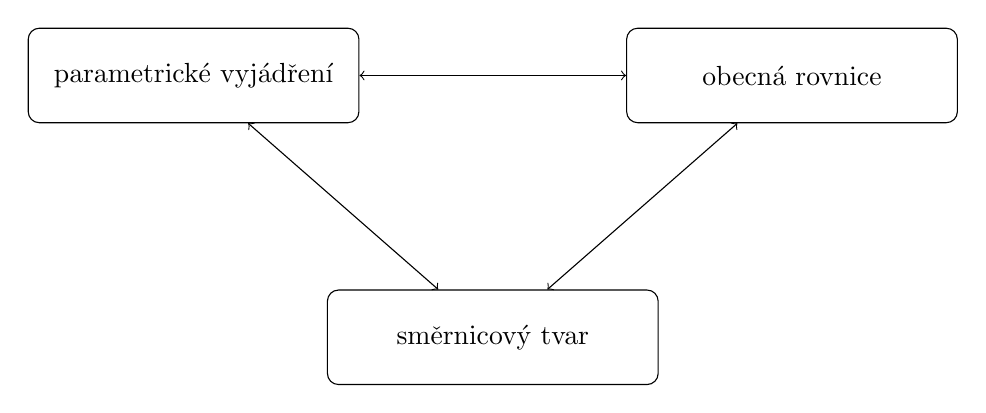
\begin{tikzpicture}[scale=0.95, every node/.style={align=center}]

        \node[
            draw,
            rounded corners,
            minimum width=4.2cm,
            minimum height=1.2cm
        ] (parametric) at (-4,1.5)
        {parametrické vyjádření};

        \node[
            draw,
            rounded corners,
            minimum width=4.2cm,
            minimum height=1.2cm
        ] (general) at (4,1.5)
        {obecná rovnice};

        \node[
            draw,
            rounded corners,
            minimum width=4.2cm,
            minimum height=1.2cm
        ] (slope) at (0,-2)
        {směrnicový tvar};

        \draw[<->] (parametric) -- (general);
        \draw[<->] (parametric) -- (slope);
        \draw[<->] (general) -- (slope);

    \end{tikzpicture}
    \caption{Převody mezi jednotlivými tvary rovnice přímky.}
    \label{fig:Conversions_between_line_forms}
\end{figure}


\subsubsection{Převod mezi parametrickým vyjádřením a obecnou rovnicí}
\label{subsubsec:Conversion_parametric_general}

\paragraph{Z parametrického vyjádření do obecné rovnice}

Uvažujme přímku zadanou parametricky ve tvaru
\begin{equation}\label{eq:Conversion_parametric_form}
    \begin{aligned}
        x&=x_A+t u_x,\\
        y&=y_A+t u_y,
        \qquad t\in\mathbb{R},
    \end{aligned}
\end{equation}
kde $A[x_A;y_A]$ je bod přímky a
\[
    \vec{u}=(u_x;u_y)
\]
je její nenulový směrový vektor.

K tomuto směrovému vektoru zvolíme kolmý normálový vektor
\[
    \vec{n}=(u_y;-u_x).
\]
Přímka prochází bodem $A[x_A;y_A]$, a proto můžeme použít rovnici
určenou bodem a normálovým vektorem:
\[
    u_y(x-x_A)-u_x(y-y_A)=0.
\]

Po roznásobení dostáváme
\begin{align*}
    u_yx-u_yx_A-u_xy+u_xy_A&=0,\\
    u_yx-u_xy+u_xy_A-u_yx_A&=0.
\end{align*}

Obecná rovnice přímky má tedy tvar
\begin{equation}\label{eq:Conversion_parametric_to_general}
    u_yx-u_xy+u_xy_A-u_yx_A=0.
\end{equation}

Její koeficienty můžeme zapsat jako
\[
    a=u_y,
    \qquad
    b=-u_x,
    \qquad
    c=u_xy_A-u_yx_A.
\]

Zvolili-li bychom opačně orientovaný normálový vektor
\[
    \vec{n}=(-u_y;u_x),
\]
získali bychom rovnici vynásobenou číslem $-1$. Obě rovnice by však
popisovaly tutéž přímku.

\begin{example}\label{exa:Conversion_parametric_to_general}
    Převeďte parametrické vyjádření přímky
    \[
        \begin{aligned}
            p:\quad x&=-2+3t,\\
                     y&=1+2t,
                     \qquad t\in\mathbb{R},
        \end{aligned}
    \]
    na obecnou rovnici.

    Z parametrického vyjádření získáme bod
    \[
        A[-2;1]
    \]
    a směrový vektor
    \[
        \vec{u}=(3;2).
    \]

    K němu zvolíme normálový vektor
    \[
        \vec{n}=(2;-3).
    \]

    Rovnici přímky zapíšeme pomocí bodu $A[-2;1]$ a normálového
    vektoru:
    \begin{align*}
        2(x-(-2))-3(y-1)&=0,\\
        2(x+2)-3(y-1)&=0,\\
        2x+4-3y+3&=0,\\
        2x-3y+7&=0.
    \end{align*}

    Obecná rovnice přímky je tedy
    \[
        p:2x-3y+7=0.
    \]

    Správnost můžeme ověřit například bodem odpovídajícím hodnotě
    $t=1$:
    \[
        P[1;3].
    \]
    Po dosazení do obecné rovnice dostáváme
    \[
        2\cdot1-3\cdot3+7=2-9+7=0.
    \]
\end{example}

\begin{remark}\label{rem:Eliminating_parameter_line_conversion}
    Parametr lze odstranit také přímým algebraickým postupem. Pokud
    například platí $u_x\neq0$, můžeme z první parametrické rovnice
    vyjádřit
    \[
        t=\frac{x-x_A}{u_x}
    \]
    a tento vztah dosadit do druhé rovnice.

    Postup pomocí normálového vektoru je však jednotný a funguje také
    pro vodorovné a svislé přímky, aniž bychom museli rozlišovat, která
    souřadnice směrového vektoru je nulová.
\end{remark}


\paragraph{Z obecné rovnice do parametrického vyjádření}

Uvažujme přímku zadanou obecnou rovnicí
\begin{equation}\label{eq:Conversion_general_form}
    ax+by+c=0,
    \qquad
    (a;b)\neq(0;0).
\end{equation}

Z koeficientů obecné rovnice získáme normálový vektor
\[
    \vec{n}=(a;b).
\]
Jako směrový vektor přímky můžeme zvolit například
\[
    \vec{u}=(-b;a).
\]

Dále potřebujeme určit alespoň jeden bod
\[
    A[x_A;y_A],
\]
který obecnou rovnici splňuje. Jeho souřadnice můžeme získat vhodnou
volbou jedné souřadnice a dopočítáním druhé.

Jakmile známe bod $A$ a směrový vektor $\vec{u}=(-b;a)$, dostáváme
parametrické vyjádření
\begin{equation}\label{eq:Conversion_general_to_parametric}
    \begin{aligned}
        x&=x_A-bt,\\
        y&=y_A+at,
        \qquad t\in\mathbb{R}.
    \end{aligned}
\end{equation}

\begin{example}\label{exa:Conversion_general_to_parametric}
    Převeďte obecnou rovnici
    \[
        q:3x-4y+5=0
    \]
    na parametrické vyjádření.

    Normálový vektor přímky je
    \[
        \vec{n}=(3;-4).
    \]
    Jako směrový vektor zvolíme
    \[
        \vec{u}=(4;3).
    \]

    Nyní určíme jeden bod přímky. Zvolíme například $x=1$:
    \begin{align*}
        3\cdot1-4y+5&=0,\\
        8-4y&=0,\\
        y&=2.
    \end{align*}

    Přímka tedy prochází bodem
    \[
        A[1;2].
    \]

    Parametrické vyjádření je
    \[
        \begin{aligned}
            q:\quad x&=1+4t,\\
                     y&=2+3t,
                     \qquad t\in\mathbb{R}.
        \end{aligned}
    \]

    Ověření provedeme dosazením parametrických rovnic do původní
    obecné rovnice:
    \begin{align*}
        3(1+4t)-4(2+3t)+5
        &=
        3+12t-8-12t+5\\
        &=
        0.
    \end{align*}

    Obecná rovnice je tedy splněna pro každé
    $t\in\mathbb{R}$.
\end{example}

\begin{remark}\label{rem:Choosing_point_general_to_parametric}
    Bod přímky můžeme určit různými způsoby. Je-li $b\neq0$, můžeme
    například položit $x=0$ a získat bod
    \[
        A\left[0;-\frac{c}{b}\right].
    \]
    Je-li $a\neq0$, můžeme položit $y=0$ a získat bod
    \[
        B\left[-\frac{c}{a};0\right].
    \]

    Někdy je však výhodnější zvolit jinou hodnotu souřadnice tak, aby
    výsledný bod měl celočíselné souřadnice.
\end{remark}


\subsubsection{Převod mezi obecnou rovnicí a směrnicovým tvarem}
\label{subsubsec:Conversion_general_slope}

\paragraph{Z obecné rovnice do směrnicového tvaru}

Uvažujme obecnou rovnici přímky
\[
    ax+by+c=0.
\]

Chceme-li ji převést do směrnicového tvaru, musíme z rovnice vyjádřit
proměnnou $y$. To je možné právě tehdy, když
\[
    b\neq0.
\]

Postupně dostáváme
\begin{align*}
    ax+by+c&=0,\\
    by&=-ax-c,\\
    y&=-\frac{a}{b}x-\frac{c}{b}.
\end{align*}

Porovnáním s rovnicí
\[
    y=kx+q
\]
získáme
\begin{equation}\label{eq:Conversion_general_to_slope}
    k=-\frac{a}{b},
    \qquad
    q=-\frac{c}{b}.
\end{equation}

\begin{example}\label{exa:Conversion_general_to_slope}
    Převeďte obecnou rovnici
    \[
        p:2x+3y-6=0
    \]
    do směrnicového tvaru.

    Vyjádříme proměnnou $y$:
    \begin{align*}
        2x+3y-6&=0,\\
        3y&=-2x+6,\\
        y&=-\frac{2}{3}x+2.
    \end{align*}

    Směrnicový tvar přímky je tedy
    \[
        p:y=-\frac{2}{3}x+2.
    \]

    Ze zápisu přímo získáme směrnici
    \[
        k=-\frac{2}{3}
    \]
    a průsečík s osou $y$
    \[
        P_y[0;2].
    \]
\end{example}


\paragraph{Ze směrnicového tvaru do obecné rovnice}

Uvažujme přímku ve směrnicovém tvaru
\[
    y=kx+q.
\]

Převedeme-li všechny členy na jednu stranu, dostáváme
\begin{equation}\label{eq:Conversion_slope_to_general}
    kx-y+q=0.
\end{equation}

Tato rovnice je obecnou rovnicí přímky. Obsahuje-li směrnice nebo
absolutní člen zlomky, můžeme celou rovnici vynásobit vhodným
nenulovým číslem a zlomky odstranit.

\begin{example}\label{exa:Conversion_slope_to_general}
    Převeďte směrnicový tvar
    \[
        q:y=-\frac{3}{4}x+2
    \]
    na obecnou rovnici.

    Převedeme všechny členy na levou stranu:
    \[
        \frac{3}{4}x+y-2=0.
    \]

    Abychom odstranili zlomek, vynásobíme celou rovnici číslem $4$:
    \[
        3x+4y-8=0.
    \]

    Obecná rovnice přímky je tedy
    \[
        q:3x+4y-8=0.
    \]

    Rovnice
    \[
        \frac{3}{4}x+y-2=0
    \]
    a
    \[
        3x+4y-8=0
    \]
    jsou navzájem ekvivalentní, protože druhá vznikla vynásobením
    první rovnice nenulovým číslem $4$.
\end{example}


\subsubsection{Převod mezi parametrickým vyjádřením a směrnicovým tvarem}
\label{subsubsec:Conversion_parametric_slope}

\paragraph{Z parametrického vyjádření do směrnicového tvaru}

Uvažujme parametrické vyjádření
\[
    \begin{aligned}
        x&=x_A+t u_x,\\
        y&=y_A+t u_y,
        \qquad t\in\mathbb{R}.
    \end{aligned}
\]

Jestliže platí
\[
    u_x\neq0,
\]
není přímka svislá a její směrnice je dána poměrem souřadnic směrového
vektoru:
\[
    k=\frac{u_y}{u_x}.
\]

Přímka prochází bodem $A[x_A;y_A]$, a proto můžeme použít
bodově-směrnicový tvar
\[
    y-y_A=k(x-x_A).
\]

Po dosazení směrnice dostáváme
\[
    y-y_A
    =
    \frac{u_y}{u_x}(x-x_A),
\]
a tedy
\begin{equation}\label{eq:Conversion_parametric_to_slope}
    y
    =
    \frac{u_y}{u_x}x
    +
    y_A
    -
    \frac{u_y}{u_x}x_A.
\end{equation}

Z toho plyne
\[
    k=\frac{u_y}{u_x},
    \qquad
    q=y_A-\frac{u_y}{u_x}x_A.
\]

\begin{example}\label{exa:Conversion_parametric_to_slope}
    Vraťme se k přímce z příkladu
    \ref{exa:Conversion_parametric_to_general}:
    \[
        \begin{aligned}
            p:\quad x&=-2+3t,\\
                     y&=1+2t,
                     \qquad t\in\mathbb{R}.
        \end{aligned}
    \]

    Její směrový vektor je
    \[
        \vec{u}=(3;2),
    \]
    a proto je její směrnice
    \[
        k=\frac{2}{3}.
    \]

    Přímka prochází bodem $A[-2;1]$, takže
    \begin{align*}
        q
        &=
        y_A-kx_A\\
        &=
        1-\frac{2}{3}\cdot(-2)\\
        &=
        1+\frac{4}{3}\\
        &=
        \frac{7}{3}.
    \end{align*}

    Směrnicový tvar přímky je
    \[
        p:y=\frac{2}{3}x+\frac{7}{3}.
    \]

    Po vynásobení rovnice číslem $3$ a převedení všech členů na jednu
    stranu získáme
    \[
        2x-3y+7=0,
    \]
    což je stejná obecná rovnice jako v příkladu
    \ref{exa:Conversion_parametric_to_general}.
\end{example}


\paragraph{Ze směrnicového tvaru do parametrického vyjádření}

Uvažujme přímku
\[
    y=kx+q.
\]

Z jejího směrnicového tvaru přímo získáme bod
\[
    Q[0;q].
\]

Jako směrový vektor můžeme zvolit
\[
    \vec{u}=(1;k),
\]
protože při zvětšení souřadnice $x$ o jednu jednotku se souřadnice
$y$ změní o hodnotu $k$.

Parametrické vyjádření proto můžeme zapsat ve tvaru
\begin{equation}\label{eq:Conversion_slope_to_parametric}
    \begin{aligned}
        x&=t,\\
        y&=q+kt,
        \qquad t\in\mathbb{R}.
    \end{aligned}
\end{equation}

Obsahuje-li směrnice zlomek, můžeme směrový vektor vynásobit vhodným
nenulovým číslem a získat tak vektor s celočíselnými souřadnicemi.

\begin{example}\label{exa:Conversion_slope_to_parametric}
    Převeďte směrnicový tvar
    \[
        r:y=-\frac{3}{2}x+4
    \]
    na parametrické vyjádření.

    Přímka prochází bodem
    \[
        Q[0;4].
    \]

    Ze směrnice můžeme nejprve získat směrový vektor
    \[
        \vec{u}_1=\left(1;-\frac{3}{2}\right).
    \]
    Abychom odstranili zlomek, vynásobíme tento vektor číslem $2$:
    \[
        \vec{u}=(2;-3).
    \]

    Parametrické vyjádření přímky je tedy
    \[
        \begin{aligned}
            r:\quad x&=2t,\\
                     y&=4-3t,
                     \qquad t\in\mathbb{R}.
        \end{aligned}
    \]

    Ověření provedeme dosazením parametrických rovnic do směrnicového
    tvaru:
    \[
        -\frac{3}{2}(2t)+4=-3t+4,
    \]
    což je právě druhá parametrická rovnice.
\end{example}


\subsubsection{Svislé přímky při převodech}
\label{subsubsec:Vertical_lines_conversions}

Svislé přímky vyžadují při převodech zvláštní pozornost. Přímka
rovnoběžná s osou $y$ má rovnici
\begin{equation}\label{eq:Vertical_line_equation_conversion}
    x=d,
    \qquad d\in\mathbb{R}.
\end{equation}

V obecném tvaru ji můžeme zapsat například jako
\[
    x-d=0.
\]
Jejím normálovým vektorem je
\[
    \vec{n}=(1;0)
\]
a směrovým vektorem například
\[
    \vec{u}=(0;1).
\]

Parametrické vyjádření svislé přímky můžeme zapsat jako
\begin{equation}\label{eq:Vertical_line_parametric_conversion}
    \begin{aligned}
        x&=d,\\
        y&=t,
        \qquad t\in\mathbb{R}.
    \end{aligned}
\end{equation}

Směrnicový tvar však pro svislou přímku neexistuje. Ze směrového
vektoru $\vec{u}=(0;1)$ bychom totiž měli získat směrnici
\[
    k=\frac{u_y}{u_x}=\frac{1}{0},
\]
což není definováno. Stejně tak svislá přímka není grafem žádné funkce
$y=f(x)$, protože jedné hodnotě $x=d$ odpovídá nekonečně mnoho hodnot
$y$.

\begin{example}\label{exa:Vertical_line_conversion}
    Převeďte obecnou rovnici
    \[
        p:2x-6=0
    \]
    na ostatní možné tvary.

    Po vydělení rovnice číslem $2$ získáme
    \[
        x-3=0,
    \]
    tedy
    \[
        x=3.
    \]

    Přímka prochází například bodem $A[3;0]$ a má směrový vektor
    \[
        \vec{u}=(0;1).
    \]

    Její parametrické vyjádření je
    \[
        \begin{aligned}
            p:\quad x&=3,\\
                     y&=t,
                     \qquad t\in\mathbb{R}.
        \end{aligned}
    \]

    Směrnicový tvar této přímky neexistuje, protože přímka je
    rovnoběžná s osou $y$.
\end{example}

\begin{remark}\label{rem:Horizontal_line_all_forms}
    Vodorovné přímky tento problém nemají. Přímku
    \[
        y=d
    \]
    můžeme zapsat všemi třemi způsoby:
    \[
        \begin{aligned}
            &\text{parametricky:}
            &&
            x=t,\quad y=d,
            \qquad t\in\mathbb{R},\\
            &\text{obecně:}
            &&
            y-d=0,\\
            &\text{směrnicově:}
            &&
            y=0x+d.
        \end{aligned}
    \]
    Její směrnice je tedy $k=0$.
\end{remark}

\begin{example}\label{exa:Line_forms_conversion_summary}
    Je dána přímka parametrickým vyjádřením
    \[
        \begin{aligned}
            p:\quad x&=1+2t,\\
                     y&=-2+3t,
                     \qquad t\in\mathbb{R}.
        \end{aligned}
    \]

    \begin{enumerate}[label=\alph*)]
        \item Určete obecnou rovnici přímky.
        \item Určete její směrnicový tvar.
        \item Ze získaného směrnicového tvaru sestavte jiné
        parametrické vyjádření téže přímky.
        \item Ověřte, že obě parametrická vyjádření popisují tutéž
        přímku.
    \end{enumerate}

    \begin{enumerate}[label=\alph*), leftmargin=2em]

        \item \textbf{Obecná rovnice}

        Z parametrického vyjádření získáme bod
        \[
            A[1;-2]
        \]
        a směrový vektor
        \[
            \vec{u}=(2;3).
        \]

        K němu zvolíme normálový vektor
        \[
            \vec{n}=(3;-2).
        \]

        Rovnici určenou bodem a normálovým vektorem zapíšeme jako
        \begin{align*}
            3(x-1)-2(y-(-2))&=0,\\
            3(x-1)-2(y+2)&=0,\\
            3x-3-2y-4&=0,\\
            3x-2y-7&=0.
        \end{align*}

        Obecná rovnice přímky je
        \[
            p:3x-2y-7=0.
        \]

        \item \textbf{Směrnicový tvar}

        Z obecné rovnice vyjádříme proměnnou $y$:
        \begin{align*}
            3x-2y-7&=0,\\
            -2y&=-3x+7,\\
            y&=\frac{3}{2}x-\frac{7}{2}.
        \end{align*}

        Směrnicový tvar přímky je
        \[
            p:y=\frac{3}{2}x-\frac{7}{2}.
        \]

        Stejný výsledek můžeme získat přímo z parametrického
        vyjádření:
        \[
            k=\frac{3}{2}
        \]
        a
        \[
            q
            =
            -2-\frac{3}{2}\cdot1
            =
            -\frac{7}{2}.
        \]

        \item \textbf{Jiné parametrické vyjádření}

        Ze směrnicového tvaru přímo získáme bod
        \[
            B\left[0;-\frac{7}{2}\right].
        \]

        Směrnici
        \[
            k=\frac{3}{2}
        \]
        odpovídá například směrový vektor
        \[
            \vec{v}=(2;3).
        \]

        Jiné parametrické vyjádření téže přímky je proto
        \[
            \begin{aligned}
                p:\quad x&=2s,\\
                         y&=-\frac{7}{2}+3s,
                         \qquad s\in\mathbb{R}.
            \end{aligned}
        \]

        \item \textbf{Ověření ekvivalence}

        Původní a nové parametrické vyjádření používají stejný směrový
        vektor
        \[
            \vec{u}=\vec{v}=(2;3).
        \]

        Stačí tedy ověřit, že bod
        \[
            B\left[0;-\frac{7}{2}\right]
        \]
        leží na původní přímce. Z první parametrické rovnice získáme
        \[
            0=1+2t,
            \qquad
            t=-\frac{1}{2}.
        \]

        Pro tuto hodnotu parametru dostáváme z druhé rovnice
        \[
            y
            =
            -2+3\left(-\frac{1}{2}\right)
            =
            -2-\frac{3}{2}
            =
            -\frac{7}{2}.
        \]

        Bod $B$ tedy na původní přímce leží, a obě parametrická
        vyjádření proto popisují tutéž přímku.

        Ekvivalenci můžeme vyjádřit také substitucí
        \[
            s=t+\frac{1}{2}.
        \]
        Potom
        \begin{align*}
            2s
            &=
            2\left(t+\frac{1}{2}\right)
            =
            1+2t,\\
            -\frac{7}{2}+3s
            &=
            -\frac{7}{2}
            +3\left(t+\frac{1}{2}\right)\\
            &=
            -\frac{7}{2}+3t+\frac{3}{2}\\
            &=
            -2+3t.
        \end{align*}
    \end{enumerate}

    Všechny tři zápisy
    \[
        \begin{aligned}
            x&=1+2t,\\
            y&=-2+3t,
            \qquad t\in\mathbb{R},
        \end{aligned}
    \]
    \[
        3x-2y-7=0
    \]
    a
    \[
        y=\frac{3}{2}x-\frac{7}{2}
    \]
    tedy popisují tutéž přímku.
\end{example}

\subsection{Polohové vztahy přímek v rovině}
\label{subsec:Positional_relations_lines_plane}

Dosud jsme se zabývali především popisem jedné přímky. Nyní budeme
uvažovat dvě přímky v téže rovině a určovat jejich vzájemnou polohu.

Při řešení budeme využívat údaje, které jednotlivé tvary rovnic
poskytují: směrové vektory, normálové vektory a směrnice. V případě
různoběžných přímek budeme také určovat jejich průsečík.

\subsubsection{Možné vzájemné polohy dvou přímek}
\label{subsubsec:Possible_relative_positions_lines}

Dvě přímky v rovině mohou být \textbf{různoběžné},
\textbf{rovnoběžné} nebo \textbf{totožné}. Mimoběžné přímky,
které nemají společný bod a zároveň nejsou rovnoběžné, se mohou
vyskytovat až v prostoru.

\begin{definition}\label{def:Intersecting_lines_plane}
    Dvě přímky v rovině nazýváme \textbf{různoběžnými}, jestliže mají
    právě jeden společný bod, který nazýváme jejich
    \textbf{průsečíkem}.
\end{definition}

\begin{definition}\label{def:Parallel_lines_plane}
    Dvě různé přímky v rovině nazýváme \textbf{rovnoběžnými}, jestliže
    mají stejný směr a nemají žádný společný bod.
\end{definition}

\begin{definition}\label{def:Coincident_lines_plane}
    Dvě přímky v rovině nazýváme \textbf{totožnými}, jestliže mají
    všechny body společné, a představují tedy tutéž množinu bodů.
\end{definition}

Jednotlivé možné vzájemné polohy dvou přímek v rovině jsou znázorněny
na obrázku \ref{fig:Relative_positions_lines_plane}.

\begin{figure}[H]
    \centering

    % -------------------------------------------------
    % Různoběžné přímky
    % -------------------------------------------------
    \begin{minipage}{0.32\textwidth}
        \centering
        \begin{tikzpicture}[scale=0.9]

            \coordinate (P) at (0,0);

            \draw[thin, <->] (-2,-1.2) -- (2,1.2)
                node[above right] {$p$};

            \draw[thin, <->] (-1.8,1.5) -- (1.8,-1.5)
                node[below right] {$q$};

            \fill (P) circle (2pt)
                node[below] {$P$};

            \draw[vector] (0.5,0.3) -- (1.5,0.91) node[midway, above, sloped]{$\vec{u}_p$};
            \draw[vector] (-0.5,0.4) -- (-1.2,1) node[midway, above, sloped] {$\vec{u}_q$};

        \end{tikzpicture}

        \small různoběžné
    \end{minipage}
    \hfill
    % -------------------------------------------------
    % Rovnoběžné přímky
    % -------------------------------------------------
    \begin{minipage}{0.32\textwidth}
        \centering
        \begin{tikzpicture}[scale=0.9]

            \draw[thin, <->] (-2,0.7) -- (2,0.7)
                node[above right] {$p$};

            \draw[thin, <->] (-2,-0.7) -- (2,-0.7)
                node[above right] {$q$};

            \draw[vector] (0.5,0.7) -- (1.2,0.7) node[midway, above, sloped]{$\vec{u}_p$};
            \draw[vector] (0.2,-0.7) -- (-1,-0.7) node[midway, above, sloped] {$\vec{u}_q$};

        \end{tikzpicture}

        \small rovnoběžné
    \end{minipage}
    \hfill
    % -------------------------------------------------
    % Totožné přímky
    % -------------------------------------------------
    \begin{minipage}{0.32\textwidth}
        \centering
        \begin{tikzpicture}[scale=0.9]

            \draw[thin, <->] (-2,0) -- (2,0);
            \node[below right] at (1.2,0) {$p = q$};

            \draw[vector] (-0.5,0) -- (-1.75,0) node[midway, above, sloped]{$\vec{u}_p$};
            \draw[vector] (1,0) -- (1.7,0) node[midway, above, sloped] {$\vec{u}_q$};

        \end{tikzpicture}

        \small totožné
    \end{minipage}

    \caption{Možné vzájemné polohy dvou přímek v rovině.}
    \label{fig:Relative_positions_lines_plane}
\end{figure}

\subsubsection{Vzájemná poloha parametricky zadaných přímek}
\label{subsubsec:Relative_position_parametric_lines}

U parametrického vyjádření je směr přímky určen jejím směrovým
vektorem. Vzájemnou polohu dvou parametricky zadaných přímek proto
budeme určovat především porovnáním jejich směrových vektorů.

Uvažujme přímky $p$ a $q$ zadané parametricky ve tvaru
\begin{align}
    p: X &= A+t\vec{u},
    \qquad t\in\mathbb{R},
    \label{eq:Parametric_line_p_relative_position}\\
    q: X &= B+s\vec{v},
    \qquad s\in\mathbb{R},
    \label{eq:Parametric_line_q_relative_position}
\end{align}
kde $A$ a $B$ jsou zvolené body jednotlivých přímek a $\vec{u}$,
$\vec{v}$ jsou jejich nenulové směrové vektory.

Pro každou přímku používáme jiný parametr, v našem případě $t$ a $s$,
protože hodnota parametru určuje, o jaký násobek příslušného směrového
vektoru se ze zvoleného bodu posuneme. Hodnota parametru potřebná
k dosažení společného bodu z bodu $A$ proto obecně nemusí být stejná
jako hodnota parametru potřebná k dosažení téhož bodu z bodu $B$.

Vzájemnou polohu přímek určíme nejprve porovnáním jejich směrových
vektorů.

Jestliže směrové vektory $\vec{u}$ a $\vec{v}$ nejsou rovnoběžné,
tedy neexistuje číslo $k\in\mathbb{R}$, pro které by platilo
\[
    \vec{v}=k\vec{u},
\]
mají přímky různé směry. Protože obě přímky leží v jedné rovině,
protínají se právě v jednom bodě a jsou tedy různoběžné podle definice \ref{def:Intersecting_lines_plane}.

Jestliže naopak existuje číslo
$k\in\mathbb{R}\setminus\{0\}$ takové, že
\[
    \vec{v}=k\vec{u},
\]
mají přímky stejný směr. V takovém případě jsou přímky buď rovnoběžné,
nebo totožné, a proto musíme ještě ověřit, zda jeden zvolený bod jedné
přímky leží také na přímce druhé.

Pokud zvolený bod $B$ přímky $q$ neleží na přímce $p$,
nemají přímky žádný společný bod a jsou proto rovnoběžné podle definice \ref{def:Parallel_lines_plane}. 
Jestliže naopak bod $B$ na přímce $p$ leží, mají obě přímky
společný bod a zároveň stejný směr, takže jsou totožné podle definice \ref{def:Coincident_lines_plane}.

Celý rozhodovací postup můžeme shrnout následovně:
\[
\begin{array}{c|c}
\text{Podmínka}
&
\text{Vzájemná poloha přímek}
\\
\hline
\vec{u}\text{ a }\vec{v}\text{ nejsou rovnoběžné}
&
\text{přímky jsou různoběžné}
\\[1mm]
\vec{v}=k\vec{u},\ k\neq0,\ \text{a }B\notin p
&
\text{přímky jsou rovnoběžné}
\\[1mm]
\vec{v}=k\vec{u},\ k\neq0,\ \text{a }B\in p
&
\text{přímky jsou totožné}
\end{array}
\]
Rozhodovací postup můžeme také shrnout pomocí schématu na obrázku
\ref{fig:Relative_position_parametric_lines_decision}.

\begin{remark}\label{rem:Alternative_test_coincident_lines}
    Místo přímého dosazování bodu $B$ do parametrického vyjádření
    přímky $p$ můžeme určit vektor
    \[
        \overrightarrow{AB}=B-A.
    \]
    Bod $B$ leží na přímce $p$ právě tehdy, když existuje číslo
    $\lambda\in\mathbb{R}$ takové, že
    \[
        \overrightarrow{AB}=\lambda\vec{u}.
    \]
    Tato podmínka zahrnuje také případ $A=B$, pro který je
    $\lambda=0$.

    Jsou-li současně směrové vektory obou přímek rovnoběžné, jsou
    přímky totožné. Dosazování bodu do parametrického vyjádření však
    zároveň procvičuje postup potřebný při hledání průsečíku, a proto
    jej budeme v následujících příkladech používat častěji.
\end{remark}

\begin{figure}[H]
    \centering
    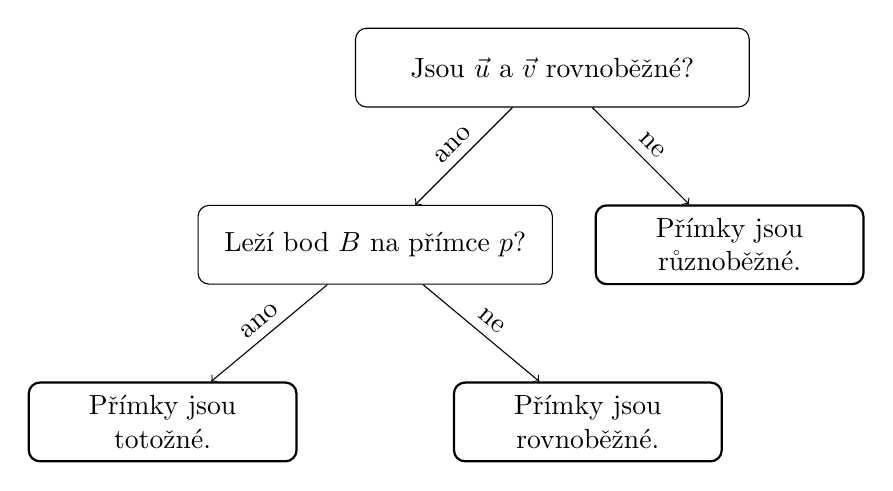
\begin{tikzpicture}[scale=0.9, every node/.style={align=center}]

        % Uzly
        \node[draw, rounded corners, minimum width=5cm, minimum height=1cm]
            (start) at (0,0)
            {Jsou $\vec{u}$ a $\vec{v}$ rovnoběžné?};

        \node[draw, rounded corners, minimum width=4.5cm, minimum height=1cm]
            (point) at (-2.5,-2.5)
            {Leží bod $B$ na přímce $p$?};

        \node[draw, rounded corners, minimum width=3.4cm, minimum height=1cm, thick]
            (intersecting) at (2.5,-2.5)
            {Přímky jsou\\různoběžné.};

        \node[draw, rounded corners, minimum width=3.4cm, minimum height=1cm, thick]
            (coincident) at (-5.5,-5)
            {Přímky jsou\\totožné.};

        \node[draw, rounded corners, minimum width=3.4cm, minimum height=1cm, thick]
            (parallel) at (0.5,-5)
            {Přímky jsou\\rovnoběžné.};

        % Šipky
        \draw[->] (start) -- (point)
            node[midway, above, sloped] {ano};

        \draw[->] (start) -- (intersecting)
            node[midway, above, sloped] {ne};

        \draw[->] (point) -- (coincident)
            node[midway, above, sloped] {ano};

        \draw[->] (point) -- (parallel)
            node[midway, above, sloped] {ne};

    \end{tikzpicture}
    \caption{Postup při určování vzájemné polohy parametricky zadaných přímek v rovině.}
    \label{fig:Relative_position_parametric_lines_decision}
\end{figure}

\paragraph{Rovnoběžné přímky}

Jak již bylo řečeno, jsou-li směrové vektory dvou přímek navzájem rovnoběžné, nemůžeme pouze
z této skutečnosti rozhodnout, zda jsou přímky rovnoběžné, nebo totožné.
Musíme ještě ověřit, zda jeden zvolený bod jedné přímky leží také na
druhé přímce.

\begin{example}\label{exa:Parallel_parametric_lines}
    Určete vzájemnou polohu přímek $p$ a $q$ zadaných bodem
    a směrovým vektorem:
    \[
        p:\ A[-1;3],\qquad \vec{u}=(-1;2),
    \]
    \[
        q:\ B[1;1],\qquad \vec{v}=(2;-4).
    \]

    Nejprve zjistíme, zda jsou směrové vektory $\vec{u}$ a $\vec{v}$
    navzájem rovnoběžné. Hledáme tedy číslo $k\in\mathbb{R}$, pro které
    platí
    \[
        \vec{v}=k\vec{u}.
    \]

    Po dosazení souřadnic dostáváme
    \[
        (2;-4)=k(-1;2).
    \]
    Z jednotlivých souřadnic vyplývá
    \begin{align*}
        2 &= -k \Rightarrow  k=-2,\\
        -4 &= 2k \Rightarrow k=-2.
    \end{align*}

    Z obou souřadnic vyšla stejná hodnota $k=-2$, a proto jsou směrové
    vektory rovnoběžné. Přímky $p$ a $q$ jsou tedy buď rovnoběžné,
    nebo totožné.

    Nyní ověříme, zda bod $A[-1;3]$ leží na přímce $q$. Parametrické
    vyjádření přímky $q$ je
    \begin{align*}
        q: x &= 1+2s,\\
           y &= 1-4s;
           \quad s\in\mathbb{R}.
    \end{align*}

    Dosadíme souřadnice bodu $A[-1;3]$:
    \begin{align*}
        -1 &= 1+2s,\\
        3 &= 1-4s.
    \end{align*}

    Z první rovnice získáme
    \begin{align*}
        -1 &= 1+2s,\\
        -2 &= 2s,\\
        s &= -1.
    \end{align*}
    Z druhé rovnice však vychází
    \begin{align*}
        3 &= 1-4s,\\
        2 &= -4s,\\
        s &= -\tfrac{1}{2}.
    \end{align*}

    Z rovnic vyšly různé hodnoty parametru, takže bod $A$ na přímce
    $q$ neleží. Přímky mají rovnoběžné směrové vektory, ale nemají
    společný bod, a proto jsou rovnoběžné:
    \[
        p\parallel q.
    \]
\end{example}

\paragraph{Různoběžné přímky a jejich průsečík}

Jestliže směrové vektory dvou přímek nejsou navzájem rovnoběžné, jsou
přímky v rovině různoběžné a mají právě jeden společný bod. Tento bod
nazýváme \textbf{průsečíkem přímek}.

Průsečík musí současně ležet na obou přímkách, a jeho souřadnice proto
musí vyhovovat parametrickým rovnicím přímky $p$ i přímky $q$. Při
hledání průsečíku tedy položíme odpovídající souřadnice obou přímek
sobě rovny a vyřešíme vzniklou soustavu rovnic.

\begin{remark}\label{rem:Different_parameters_parametric_lines}
    Při porovnávání dvou parametricky vyjádřených přímek musíme pro
    každou přímku použít jiný parametr. Zápisy
    \[
        p:\ X=A+t\vec{u}
        \qquad\text{a}\qquad
        q:\ X=B+s\vec{v}
    \]
    proto používají parametry $t$ a $s$.

    Stejný bod může být totiž na první přímce získán například pro
    $t=1$, zatímco na druhé přímce může témuž bodu odpovídat hodnota
    $s=-1$. Použití stejného parametru v obou přímkách by znamenalo
    neoprávněný předpoklad, že se k průsečíku z obou zvolených bodů
    dostaneme pomocí stejného násobku rozdílných směrových vektorů.
\end{remark}

\begin{example}\label{exa:Intersecting_parametric_lines}
    Určete vzájemnou polohu přímek
    \[
        \begin{aligned}
            p:\quad x &= -1+3t,\\
                     y &= 1+t;
                     \quad t\in\mathbb{R}
        \end{aligned}
        \qquad\text{a}\qquad
        \begin{aligned}
            q:\quad x &= 1-s,\\
                     y &= -2s;
                     \quad s\in\mathbb{R}.
        \end{aligned}
    \]
    Jsou-li přímky různoběžné, určete jejich průsečík.

    Směrové vektory přímek jsou
    \[
        \vec{u}=(3;1),
        \qquad
        \vec{v}=(-1;-2).
    \]

    Nejprve ověříme, zda existuje číslo $k$, pro které platí
    \[
        \vec{v}=k\vec{u}.
    \]
    Z první souřadnice dostáváme
    \[
        -1=3k
        \qquad\Rightarrow\qquad
        k=-\frac13,
    \]
    zatímco z druhé souřadnice získáme
    \[
        -2=k.
    \]

    Hodnoty čísla $k$ se neshodují, takže směrové vektory nejsou
    rovnoběžné. Přímky $p$ a $q$ jsou proto různoběžné a mají právě
    jeden průsečík.

    Souřadnice průsečíku musí vyhovovat oběma parametrickým vyjádřením.
    Položíme proto odpovídající souřadnice sobě rovny:
    \begin{align*}
        p_x &= q_x,\\
        p_y &= q_y,
    \end{align*}
    což po dosazení parametrických rovnic přímek $p$ a $q$ dává soustavu
    \begin{align*}
        -1+3t &= 1-s,\\
        1+t &= -2s.
    \end{align*}

    Po úpravě získáme soustavu
    \begin{align*}
        3t+s &= 2,\\
        t+2s &= -1.
    \end{align*}

    Z první rovnice vyjádříme parametr $s$:
    \[
        s=2-3t.
    \]
    Dosadíme do druhé rovnice, abychom získali hodnotu parametru $t$:
    \begin{align*}
        t+2(2-3t) &= -1,\\
        t+4-6t &= -1,\\
        -5t &= -5,\\
        t &= 1.
    \end{align*}

    Hodnotu parametru $s$ dopočítáme zpětným dosazením do vztahu pro $s$:
    \[
        s=2-3\cdot1=-1.
    \]

    Souřadnice průsečíku nyní vypočítáme dosazením parametru $t=1$
    do parametrického vyjádření přímky $p$:
    \begin{align*}
        x &= -1+3\cdot1=2,\\
        y &= 1+1=2.
    \end{align*}

    Průsečíkem přímek je tedy bod
    \[
        P[2;2].
    \]

    Výsledek můžeme ověřit také dosazením hodnoty $s=-1$ do přímky $q$:
    \begin{align*}
        x &= 1-(-1)=2,\\
        y &= -2\cdot(-1)=2.
    \end{align*}

    Řešením soustavy rovnic pro parametry je dvojice
    \[
        (t;s)=(1;-1).
    \]
    Po dosazení jedné z těchto hodnot do odpovídajícího parametrického
    vyjádření jsme získali společný bod
    \[
        P[2;2].
    \]

    Průsečíkem přímek $p$ a $q$ je proto bod $P[2;2]$, což zapisujeme
    \[
        p\cap q=\{P[2;2]\}.
    \]
    
\end{example}

\begin{remark}\label{rem:Parameters_are_not_intersection_coordinates}
    Hodnoty parametrů $t$ a $s$ nejsou souřadnicemi průsečíku.
    Parametry pouze určují, jakým násobkem směrového vektoru se musíme
    posunout ze zvoleného bodu příslušné přímky. Souřadnice průsečíku
    získáme až následným dosazením vypočítané hodnoty parametru do
    parametrického vyjádření jedné z přímek.
\end{remark}

\paragraph{Totožné přímky}

Jsou-li směrové vektory dvou přímek rovnoběžné a zároveň jeden zvolený
bod první přímky leží na druhé přímce, obsahují obě přímky tentýž bod
a mají stejný směr. V takovém případě mají všechny body společné a jsou
totožné.

\begin{example}\label{exa:Coincident_parametric_lines}
    Určete vzájemnou polohu přímek
    \[
        \begin{aligned}
            p:\quad x &= -2 + 2t,\\
                    y &= 1 - t;
                    \quad t\in\mathbb{R}
        \end{aligned}
        \qquad\text{a}\qquad
        \begin{aligned}
            q:\quad x &= 4 - 4s,\\
                    y &= -2 + 2s;
                    \quad s\in\mathbb{R}.
        \end{aligned}
    \]
    Z parametrických rovnic vyčteme zvolené body a směrové vektory:
    \[
        A[-2;1],
        \qquad
        \vec{u}=(2;-1),
    \]
    \[
        B[4;-2],
        \qquad
        \vec{v}=(-4;2).
    \]

    Směrové vektory jsou rovnoběžné, protože
    \[
        \vec{v}=-2\vec{u}.
    \]

    Přímky jsou proto buď rovnoběžné, nebo totožné. 
    Ověříme, zda bod $A[-2;1]$ leží na přímce $q$. Dosadíme jeho souřadnice:
    \begin{align*}
        -2 &= 4-4s,\\
        1 &= -2+2s.
    \end{align*}

    Z první rovnice získáme
    \[
        s=\frac32,
    \]
    a z druhé rovnice rovněž
    \[
        s=\frac32.
    \]

    Bod $A$ tedy leží na přímce $q$. Přímky mají rovnoběžné směrové
    vektory a společný bod, a proto jsou totožné:
    \[
        p=q.
    \]

    Totožnost můžeme ověřit také řešením soustavy rovnic pro společné
    body:
    \begin{align*}
        -2+2t &= 4-4s,\\
        1-t &= -2+2s.
    \end{align*}

    Po úpravě první rovnice dostáváme
    \[
        t+2s=3,
    \]
    zatímco úpravou druhé rovnice získáme tutéž podmínku
    \[
        t+2s=3.
    \]

    Obě rovnice soustavy jsou tedy ekvivalentní, takže soustava má nekonečně mnoho řešení. 
    Každému bodu přímky odpovídá dvojice parametrů $t$ a $s$, která splňuje vztah
    \[
        t+2s=3.
    \]
    Protože má soustava nekonečně mnoho řešení, 
    mají přímky nekonečně mnoho společných bodů. Jejich průnikem je tedy celá přímka:
    \[
        p\cap q=p=q.
    \]
\end{example}

\paragraph{Kolmé přímky}

Kolmost je zvláštním případem různoběžnosti. Dvě parametricky zadané
přímky jsou kolmé právě tehdy, když jsou kolmé jejich směrové vektory.

Pro přímky se směrovými vektory $\vec{u}$ a $\vec{v}$ tedy platí
\[
    p\perp q
    \quad\Longleftrightarrow\quad
    \vec{u}\cdot\vec{v}=0.
\]

Protože jsou směrové vektory nenulové, nemohou být v tomto případě
rovnoběžné. Kolmé přímky se tedy v rovině protínají právě v jednom
bodě.

Určování průsečíku dvou parametricky vyjádřených přímek můžeme využít
také v geometrických úlohách. Typickým příkladem je výpočet souřadnic
paty výšky v trojúhelníku, protože pata výšky je průsečíkem přímky
obsahující jednu stranu trojúhelníku a přímky, která prochází protějším
vrcholem a je k této straně kolmá.

\begin{example}\label{exa:Foot_of_altitude_parametric_lines}
    Určete souřadnice paty výšky $v_c$ v trojúhelníku $ABC$, jehož
    vrcholy jsou
    \[
        A[-2;-1],\qquad B[6;-5],\qquad C[3;4].
    \]

    Výška $v_c$ je vedena z vrcholu $C$ kolmo ke straně $AB$.
    Její pata, kterou označíme $P_C$, proto leží současně na přímce
    obsahující stranu $AB$ i na výšce $v_c$. Bod $P_C$ tedy nalezneme
    jako průsečík těchto dvou přímek.

    Nejprve určíme směrový vektor přímky obsahující stranu $AB$:
    \[
        \overrightarrow{AB}
        =
        (6-(-2);-5-(-1))
        =
        (8;-4).
    \]

    Směrový vektor můžeme nahradit jeho jednodušším nenulovým násobkem:
    \[
        \vec{u}_{AB}=(2;-1).
    \]

    Přímka $p_{AB}$ procházející bodem $A[-2;-1]$ má tedy parametrické
    vyjádření
    \begin{align*}
        p_{AB}: x &= -2+2t,\\
                y &= -1-t;
                \quad t\in\mathbb{R}.
    \end{align*}

    Směrový vektor výšky $v_c$ musí být kolmý ke směrovému vektoru
    $\vec{u}_{AB}=(2;-1)$. Můžeme proto zvolit například vektor
    \[
        \vec{u}_{v_c}=(1;2),
    \]
    protože
    \[
        (2;-1)\cdot(1;2)=2-2=0.
    \]

    Výška $v_c$ prochází vrcholem $C[3;4]$, a proto má parametrické
    vyjádření
    \begin{align*}
        v_c: x &= 3+s,\\
             y &= 4+2s;
             \quad s\in\mathbb{R}.
    \end{align*}

    Pata výšky $P_C$ leží na obou přímkách, a proto musí její souřadnice
    vyhovovat oběma parametrickým vyjádřením. Položíme tedy odpovídající
    souřadnice sobě rovny:
    \begin{align*}
        -2+2t &= 3+s,\\
        -1-t &= 4+2s.
    \end{align*}

    Po úpravě získáme soustavu
    \begin{align*}
        2t-s &= 5,\\
        t+2s &= -5.
    \end{align*}

    Z první rovnice vyjádříme parametr $s$:
    \[
        s=2t-5.
    \]

    Dosadíme jej do druhé rovnice:
    \begin{align*}
        t+2(2t-5) &= -5,\\
        t+4t-10 &= -5,\\
        5t &= 5,\\
        t &= 1.
    \end{align*}

    Hodnotu parametru $s$ dopočítáme zpětným dosazením:
    \[
        s=2\cdot1-5=-3.
    \]

    Souřadnice paty výšky získáme například dosazením hodnoty $t=1$
    do parametrického vyjádření přímky $p_{AB}$:
    \begin{align*}
        x &= -2+2\cdot1=0,\\
        y &= -1-1=-2.
    \end{align*}

    Pata výšky $v_c$ má tedy souřadnice
    \[
        P_C[0;-2].
    \]

    Výsledek můžeme ověřit také dosazením hodnoty $s=-3$ do
    parametrického vyjádření výšky:
    \begin{align*}
        x &= 3+(-3)=0,\\
        y &= 4+2\cdot(-3)=-2.
    \end{align*}

    Obě parametrická vyjádření určují stejný bod, a proto je hledanou
    patou výšky skutečně bod
    \[
        P_C[0;-2].
    \]
\end{example}
\subsubsection{Vzájemná poloha přímek zadaných obecnými rovnicemi}
\label{subsubsec:Relative_position_general_lines}

U přímek zadaných obecnými rovnicemi můžeme jejich vzájemnou polohu
určovat pomocí normálových vektorů, které získáme přímo z koeficientů
u proměnných $x$ a $y$. V případě různoběžných přímek jejich průsečík
určíme řešením soustavy obou rovnic.

Uvažujme přímky
\[
    p:X=A+t\vec{u},
    \qquad
    q:X=B+s\vec{v},
    \qquad
    t,s\in\mathbb{R}.
\]

Uvažujme přímky
\begin{align}
    p &: a_1x+b_1y+c_1=0,
    \label{eq:General_line_p_relative_position}\\
    q &: a_2x+b_2y+c_2=0.
    \label{eq:General_line_q_relative_position}
\end{align}
Jejich normálové vektory jsou
\[
    \vec{n}_p=(a_1;b_1),
    \qquad
    \vec{n}_q=(a_2;b_2).
\]

Vzájemnou polohu přímek můžeme určit porovnáním jejich normálových
vektorů. Směrový vektor je s příslušnou přímkou rovnoběžný, zatímco
normálový vektor je k ní kolmý. Geometrický vztah mezi směrovými
a normálovými vektory obou přímek je znázorněn na obrázku
\ref{fig:Direction_normal_vectors_lines}.

Protože pootočením obou směrů o $90^\circ$ se jejich vzájemná
rovnoběžnost nezmění, platí
\[
    \vec{u}_p\parallel\vec{u}_q
    \quad\Longleftrightarrow\quad
    \vec{n}_p\parallel\vec{n}_q.
\]

Jestliže normálové vektory přímek nejsou rovnoběžné, nejsou rovnoběžné
ani jejich směrové vektory. Přímky proto mají různé směry a v rovině
se protínají právě v jednom bodě. Jsou tedy různoběžné podle definice
\ref{def:Intersecting_lines_plane}. Taková situace je znázorněna
na obrázku \ref{fig:Direction_normal_vectors_lines}.

Jestliže jsou naopak normálové vektory rovnoběžné, mají přímky stejný
směr. V takovém případě mohou být přímky buď rovnoběžné, nebo totožné.
K rozlišení těchto dvou možností již nestačí porovnat pouze koeficienty
$a_1$, $b_1$, $a_2$ a $b_2$, ale musíme porovnat všechny tři
koeficienty jejich obecných rovnic.

\begin{figure}[H]
    \centering
    \begin{tikzpicture}[scale=0.8]
       
        % Osy
        \draw[<->, thin]
            (-7,0) -- (4,0)
            node[right] {$x$};

        \draw[<->, thin]
            (0,-3) -- (0,5)
            node[above] {$y$};

        % Číselné hodnoty na ose x
        \foreach \x in {-6,-5,...,-1,1,2,...,4}
        {
            \draw (\x,0.08) -- (\x,-0.08);
            \node[below, font=\scriptsize] at (\x,0) {$\x$};
        }

        % Číselné hodnoty na ose y
        \foreach \y in {-3,-2,-1,1,2,...,4}
        {
            \draw (0.08,\y) -- (-0.08,\y);
            \node[left, font=\scriptsize] at (0,\y) {$\y$};
        }

        % Počátek soustavy
        \node[below left, font=\scriptsize] at (0,0) {$O$};

        % -------------------------------------------------
        % Přímka r_1: 2x - 3y + 6 = 0
        % tedy y = 2/3 x + 2
        % -------------------------------------------------

        \draw[thick, <->] (-6,-2) -- (3,4)
            node[pos=0.02, below right, black] {$p$};

        % -------------------------------------------------
        % Přímka r_2: x + 2y + 2 = 0
        % tedy y = -1/2 x - 1
        % -------------------------------------------------

        \draw[thick,<->] (-6,2) -- (2,-2)
            node[pos=0.02, below left, black] {$q$};

        % -------------------------------------------------
        % Směrový a normálový vektor přímky p
        % -------------------------------------------------

        % Společný počáteční bod
        \coordinate (C) at (-0.78,1.48);

        % Směrový vektor u_p
        \draw[vector] (C) -- (1.51385,3.00923)
            node[midway, below, sloped] {$\vec{u}_p$};

        % Normálový vektor n_p
        \draw[vector] (C) -- (-2.30923,3.77385)
            node[midway, right] {$\vec{n}_p$};

        % Ručně nakreslená značka pravého úhlu
        \draw (-0.558,1.628) -- (-0.706,1.850) -- (-0.928,1.702);

        % -------------------------------------------------
        % Směrový a normálový vektor přímky q
        % -------------------------------------------------

        % Společný počáteční bod
        \coordinate (F) at (-4.992,1.496);

        % Směrový vektor w
        \draw[vector] (F) -- (-3,0.5)
            node[midway, above, sloped] {$\vec{u}_q$};

        % Normálový vektor b
        \draw[vector] (F) -- (-3.996,3.488)
            node[midway, left] {$\vec{n}_q$};

        % Ručně nakreslená značka pravého úhlu
        \draw (-4.724,1.362) -- (-4.590,1.630) -- (-4.858,1.764);

    \end{tikzpicture}

    \caption{Směrové a normálové vektory různoběžných přímek $p$ a $q$.}
    \label{fig:Direction_normal_vectors_lines}
\end{figure}

Celý postup můžeme shrnout následovně:
\[
\begin{array}{c|c}
\text{Podmínka}
&
\text{Vzájemná poloha přímek}
\\
\hline
(a_2;b_2)\neq k(a_1;b_1)
&
\text{přímky jsou různoběžné}
\\[1mm]
(a_2;b_2)=k(a_1;b_1),\ (a_2;b_2;c_2)\neq k(a_1;b_1;c_1)
&
\text{přímky jsou rovnoběžné}
\\[1mm]
(a_2;b_2;c_2)=k(a_1;b_1;c_1)
&
\text{přímky jsou totožné}
\end{array}
\]
kde $k\in\mathbb{R}\setminus\{0\}$.

Prakticky můžeme rovnoběžnost normálových vektorů ověřit také pomocí vztahu,
což vychází z důlesku ze vztahu pro skalární součin (viz poznámka \ref{rem:Fast_orthogonal_vector})
\begin{equation}\label{eq:Parallel_general_lines_condition}
    a_1b_2-a_2b_1=0.
\end{equation}
Jestliže levá strana není rovna nule, normálové vektory nejsou
rovnoběžné a přímky jsou různoběžné.

\begin{figure}[H]
    \centering
    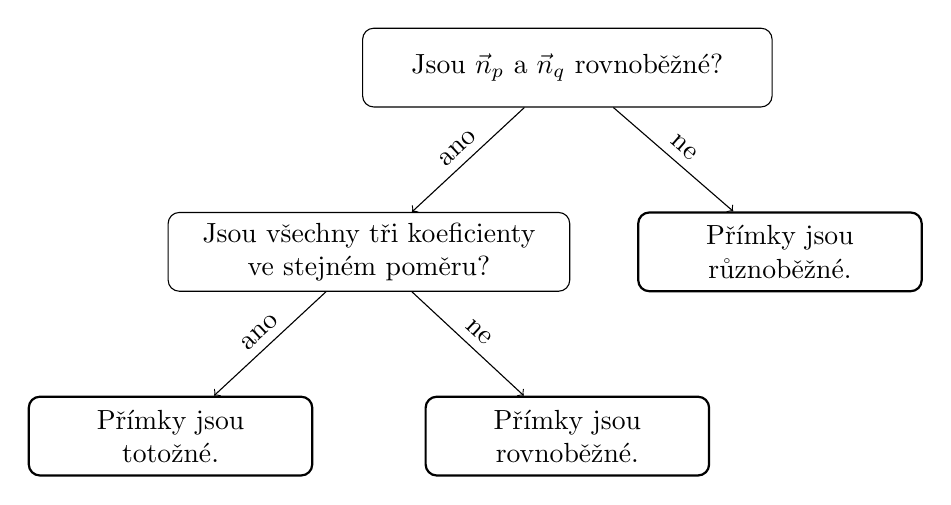
\begin{tikzpicture}[scale=0.9, every node/.style={align=center}]

        \node[draw, rounded corners, minimum width=5.2cm, minimum height=1cm]
            (start) at (0,0)
            {Jsou $\vec{n}_p$ a $\vec{n}_q$ rovnoběžné?};

        \node[draw, rounded corners, minimum width=5.1cm, minimum height=1cm]
            (coefficients) at (-2.8,-2.6)
            {Jsou všechny tři koeficienty\\ve stejném poměru?};

        \node[draw, rounded corners, minimum width=3.6cm, minimum height=1cm, thick]
            (intersecting) at (3,-2.6)
            {Přímky jsou\\různoběžné.};

        \node[draw, rounded corners, minimum width=3.6cm, minimum height=1cm, thick]
            (coincident) at (-5.6,-5.2)
            {Přímky jsou\\totožné.};

        \node[draw, rounded corners, minimum width=3.6cm, minimum height=1cm, thick]
            (parallel) at (0,-5.2)
            {Přímky jsou\\rovnoběžné.};

        \draw[->] (start) -- (coefficients)
            node[midway, above, sloped] {ano};
        \draw[->] (start) -- (intersecting)
            node[midway, above, sloped] {ne};
        \draw[->] (coefficients) -- (coincident)
            node[midway, above, sloped] {ano};
        \draw[->] (coefficients) -- (parallel)
            node[midway, above, sloped] {ne};

    \end{tikzpicture}
    \caption{Postup při určování vzájemné polohy přímek zadaných
    obecnými rovnicemi.}
    \label{fig:Relative_position_general_lines_decision}
\end{figure}

\paragraph{Rovnoběžné přímky}
\label{subsubsec:Parallel_general_lines}

Jsou-li normálové vektory dvou přímek rovnoběžné, mají přímky stejný
směr. Nejsou-li zároveň všechny tři koeficienty jejich obecných rovnic
ve stejném poměru, jde o dvě různé rovnoběžné přímky.

\begin{example}\label{exa:Parallel_general_lines}
    Určete vzájemnou polohu přímek $p:2x-3y+1=0$ a $q:-4x+6y+5=0$.
    
    Normálové vektory jsou
    \[
        \vec{n}_p=(2;-3),
        \qquad
        \vec{n}_q=(-4;6).
    \]
    Platí
    \[
        \vec{n}_q=-2\vec{n}_p,
    \]
    takže přímky mají stejný směr.

    Kdyby byly přímky totožné, musel by být stejným číslem $-2$
    vynásoben také absolutní člen. Platilo by tedy
    \[
        c_q=-2\cdot1=-2.
    \]
    Ve skutečnosti je však $c_q=5$. Všechny tři koeficienty proto
    nejsou ve stejném poměru a přímky jsou rovnoběžné:
    \[
        p\parallel q.
    \]
\end{example}

\begin{example}\label{exa:Parallel_general_line_through_point}
    Určete obecnou rovnici přímky $q$, která je rovnoběžná s přímkou $p:2x - 3y + 1 = 0$ a prochází bodem $K[-2;3]$.

    Rovnoběžná přímka může mít stejný normálový vektor
    \[
        \vec{n}_q=(2;-3).
    \]
    Její rovnice proto má tvar
    \[
        2x-3y+c=0.
    \]

    Dosadíme bod $K[-2;3]$:
    \begin{align*}
        2\cdot(-2)-3\cdot3+c&=0,\\
        -4-9+c&=0,\\
        c&=13.
    \end{align*}

    Hledaná přímka má rovnici
    \[
        q:2x-3y+13=0.
    \]
\end{example}

\paragraph{Různoběžné přímky a jejich průsečík}
\label{subsubsec:Intersecting_general_lines}

Nejsou-li normálové vektory dvou přímek rovnoběžné, mají přímky různé
směry a v rovině se protínají právě v jednom bodě. Souřadnice průsečíku
musí splňovat obě obecné rovnice současně, a proto je získáme řešením
soustavy těchto rovnic.

\begin{example}\label{exa:Intersecting_general_lines}
    Určete vzájemnou polohu přímek $p:2x+y-1=0$ a $q:x-y-2=0$.
    Jsou-li přímky různoběžné, určete jejich průsečík.

    Normálové vektory jsou
    \[
        \vec{n}_p=(2;1),
        \qquad
        \vec{n}_q=(1;-1).
    \]
    Tyto vektory nejsou rovnoběžné, protože neexistuje číslo $k$, pro
    které by platilo
    \[
        (1;-1)=k(2;1).
    \]
    Přímky jsou tedy různoběžné.

    Průsečík získáme řešením soustavy
    \begin{align*}
        2x+y-1&=0,\\
        x-y-2&=0.
    \end{align*}
    Po úpravě dostáváme
    \begin{align*}
        2x+y&=1,\\
        x-y&=2.
    \end{align*}

    Sečtením rovnic získáme
    \begin{align*}
        3x&=3,\\
        x&=1.
    \end{align*}
    Dosazením do druhé rovnice dostáváme
    \begin{align*}
        1-y&=2,\\
        y&=-1.
    \end{align*}

    Přímky se protínají v bodě
    \[
        P[1;-1],
    \]
    a proto
    \[
        p\cap q=\{P[1;-1]\}.
    \]
\end{example}

\paragraph{Totožné přímky}
\label{subsubsec:Coincident_general_lines}

Jsou-li všechny tři koeficienty jedné obecné rovnice stejným
nenulovým násobkem koeficientů druhé rovnice, popisují obě rovnice
tutéž množinu bodů. Přímky jsou proto totožné.

\begin{example}\label{exa:Coincident_general_lines}
    Určete vzájemnou polohu přímek $p:2x-3y+1=0$ a $q:-4x+6y-2=0$.

    Pro vektory platí
    \[
        (2;-3) = -\frac{1}{2}(-4;6)
    \]
    Z toho je zřejmé, že přímky jsou buď rovnoběžné anebo totožné.
    Zjistíme, zdali bod z přímky $p$ náleží přímce $q$. Najdemte tedy bod ležící na přímce $p$,
    tak že dosadíme jednu libovolnou souřadnici, např $x = -2$ a druhou dopočítáme. 

    \begin{align*}
        2 \cdot (-2) - 3y + 1 &= 0, \\
        -4 -3y +1 &= 0, \\
        -3y &= 3, \\
        y &= -1.
    \end{align*}

    Bod ležící na přímce $p$ je tedy $P[-2;-1]$. A ověříme zdali tento bod leží i na přímce $q$.

    \begin{align*}
        -4 \cdot (-2) + 6 \cdot (-1) - 2 &= 0, \\
        8 - 6 - 2 &= 0, \\
        0 &= 0.
    \end{align*}

    Protože bod $P[-2;-1]$ náleží oběma přímkám a zároveň jejich normálové vektory jsou rovnoběžné,
    pak jsou přímky totožné.

    Další způsob řešení je využítím toho, že pro koeficienty platí
    \[
        (-4;6;-2)=-2(2;-3;1).
    \]
    Druhá rovnice tedy vznikla vynásobením první rovnice číslem $-2$.
    Obě rovnice mají stejnou množinu řešení, a proto jsou přímky
    totožné:
    \[
        p=q.
    \]
    Jejich průnikem je celá přímka:
    \[
        p\cap q=p=q.
    \]
\end{example}

\paragraph{Kolmé přímky}
\label{subsubsec:Perpendicular_general_lines}

Dvě přímky jsou kolmé právě tehdy, když jsou kolmé jejich směrové
vektory. Protože pootočením obou vektorů o $90^\circ$ se velikost úhlu
mezi nimi nezmění, můžeme kolmost ověřovat také pomocí normálových
vektorů.

Pro přímky
\[
    p:a_1x+b_1y+c_1=0
\]
a
\[
    q:a_2x+b_2y+c_2=0
\]
platí
\begin{equation}\label{eq:Perpendicular_general_lines}
    p\perp q
    \quad\Longleftrightarrow\quad
    a_1a_2+b_1b_2=0.
\end{equation}

\begin{example}\label{exa:Perpendicular_general_lines}
    Určete vzájemnou polohu přímek
    \[
        p:x+2y-5=0
    \]
    a
    \[
        q:2x-y-5=0.
    \]

    Normálové vektory jsou
    \[
        \vec{n}_p=(1;2),
        \qquad
        \vec{n}_q=(2;-1).
    \]
    Jejich skalární součin je
    \[
        \vec{n}_p\cdot\vec{n}_q
        =
        1\cdot2+2\cdot(-1)
        =
        0.
    \]
    Přímky jsou proto kolmé:
    \[
        p\perp q.
    \]

    Jejich průsečík získáme řešením soustavy
    \begin{align*}
        x+2y&=5,\\
        2x-y&=5.
    \end{align*}
    Z druhé rovnice vyjádříme
    \[
        y=2x-5
    \]
    a dosadíme do první:
    \begin{align*}
        x+2(2x-5)&=5,\\
        5x-10&=5,\\
        x&=3.
    \end{align*}
    Potom
    \[
        y=2\cdot3-5=1.
    \]
    Kolmé přímky se protínají v bodě
    \[
        P[3;1].
    \]
\end{example}

\begin{example}\label{exa:Perpendicular_general_line_through_point}
    Určete obecnou rovnici přímky $q$, která je kolmá k přímce $p:2x-3y+1=0$ a prochází bodem $K[-2;3]$.
    
    Normálový vektor přímky $p$ je
    \[
        \vec{n}_p=(2;-3).
    \]
    Směrový vektor přímky $p$ můžeme zvolit například
    \[
        \vec{u}_p=(3;2).
    \]

    Hledaná přímka $q$ má být k přímce $p$ kolmá. Její normálový vektor
    proto může být rovnoběžný se směrovým vektorem přímky $p$. Zvolíme
    \[
        \vec{n}_q=(3;2).
    \]

    Rovnice hledané přímky má tvar
    \[
        3x+2y+c=0.
    \]
    Dosadíme bod $K[-2;3]$:
    \begin{align*}
        3\cdot(-2)+2\cdot3+c&=0,\\
        -6+6+c&=0,\\
        c&=0.
    \end{align*}

    Hledaná kolmice má rovnici
    \[
        q:3x+2y=0.
    \]
\end{example}

\begin{example}\label{exa:Central_symmetry_line}
    Je dána přímka
    \[
        p:2x-y+1=0.
    \]
    Určete rovnici přímky $p'$, která je obrazem přímky $p$ ve
    středové souměrnosti se středem
    \[
        S[-2;1].
    \]

    Přímku $p'$ můžeme určit pomocí obrazů dvou různých bodů přímky
    $p$. Pro obraz libovolného bodu $X$ ve středové souměrnosti se
    středem $S$ platí
    \[
        X'=S+(S-X)=2S-X.
    \]

    Nejprve tedy na přímce $p$ zvolíme dva různé body, určíme jejich
    obrazy a následně sestavíme rovnici přímky procházející těmito
    obrazy.

    Zvolíme nejprve bod s první souřadnicí $x=0$. Dosadíme do rovnice
    přímky $p$:
    \begin{align*}
        2\cdot0-y+1&=0,\\
        -y+1&=0,\\
        y&=1.
    \end{align*}

    Na přímce $p$ tedy leží bod
    \[
        A[0;1].
    \]

    Jako druhý bod zvolíme bod s první souřadnicí $x=1$:
    \begin{align*}
        2\cdot1-y+1&=0,\\
        3-y&=0,\\
        y&=3.
    \end{align*}

    Druhým bodem přímky $p$ je
    \[
        B[1;3].
    \]

    Nyní určíme obraz bodu $A$ ve středové souměrnosti se středem
    $S[-2;1]$:
    \begin{align*}
        A'
        &=
        S+(S-A)\\
        &=
        [-2;1]+\bigl([-2;1]-[0;1]\bigr)\\
        &=
        [-2;1]+(-2;0)\\
        &=
        [-4;1].
    \end{align*}

    Obdobně určíme obraz bodu $B$:
    \begin{align*}
        B'
        &=
        S+(S-B)\\
        &=
        [-2;1]+\bigl([-2;1]-[1;3]\bigr)\\
        &=
        [-2;1]+(-3;-2)\\
        &=
        [-5;-1].
    \end{align*}

    Obrazem přímky $p$ je přímka $p'$, která prochází body
    \[
        A'[-4;1]
        \qquad\text{a}\qquad
        B'[-5;-1].
    \]

    Její směrový vektor můžeme určit jako
    \[
        \overrightarrow{A'B'}
        =
        (-5-(-4);-1-1)
        =
        (-1;-2).
    \]

    K tomuto směrovému vektoru zvolíme normálový vektor
    \[
        \vec{n}_{p'}=(2;-1),
    \]
    protože
    \[
        (-1;-2)\cdot(2;-1)
        =
        -2+2
        =
        0.
    \]

    Obecná rovnice přímky $p'$ má tedy tvar
    \[
        2x-y+c=0.
    \]

    Dosadíme například bod $A'[-4;1]$:
    \begin{align*}
        2\cdot(-4)-1+c&=0,\\
        -8-1+c&=0,\\
        c&=9.
    \end{align*}

    Hledaná přímka má rovnici
    \[
        p':2x-y+9=0.
    \]

    Přímky $p$ a $p'$ mají stejné normálové vektory, a jsou proto
    rovnoběžné. To odpovídá vlastnosti středové souměrnosti: obrazem
    přímky, která neprochází středem souměrnosti, je přímka s ní
    rovnoběžná.

    \begin{figure}[H]
        \centering
        \begin{tikzpicture}[scale=0.9]

            % Přímky
            \draw[thin, <->]
                (-1.5,-2) -- (2.5,6)
                node[above right] {$p$};

            \draw[thin, <->]
                (-5.5,-2) -- (-1.5,6)
                node[above right] {$p'$};

            % Body
            \coordinate (A) at (0,1);
            \coordinate (B) at (1,3);
            \coordinate (S) at (-2,1);
            \coordinate (Ap) at (-4,1);
            \coordinate (Bp) at (-5,-1);

            \fill (A) circle (2.5pt)
                node[below right] {$A$};
            \fill (B) circle (2.5pt)
                node[below right] {$B$};
            \fill (S) circle (2.5pt)
                node[above right] {$S$};
            \fill (Ap) circle (2.5pt)
                node[above left] {$A'$};
            \fill (Bp) circle (2.5pt)
                node[below left] {$B'$};

            % Spojnice bodů se středem
            \draw[vector] (A) -- (S);
            \draw[vector] (S) -- (Ap);

            \draw[vector] (B) -- (S);
            \draw[vector] (S) -- (Bp);

        \end{tikzpicture}
        \caption{Přímka $p'$ je obrazem přímky $p$ ve středové
        souměrnosti se středem $S$.}
        \label{fig:Central_symmetry_line}
    \end{figure}
\end{example}
\subsubsection{Vzájemná poloha přímek ve směrnicovém tvaru}
\label{subsubsec:Relative_position_slope_intercept_lines}

Ve směrnicovém tvaru je směr přímky určen přímo její směrnicí.
Vzájemnou polohu dvou nesvislých přímek proto můžeme určit porovnáním
jejich směrnic a úseků na ose $y$.

Uvažujme dvě přímky
\begin{align*}
    p &: y=k_1x+q_1,\\
    q &: y=k_2x+q_2.
\end{align*}

Jejich směr určují směrnice $k_1$ a $k_2$.

Jestliže
\[
    k_1\neq k_2,
\]
mají přímky různé směry, a proto jsou různoběžné. Jejich průsečík
získáme řešením rovnice
\[
    k_1x+q_1=k_2x+q_2.
\]

Odtud
\begin{equation}\label{eq:Slope_intercept_intersection_x}
    x_P=\frac{q_2-q_1}{k_1-k_2}.
\end{equation}

Druhou souřadnici průsečíku získáme dosazením hodnoty $x_P$ do rovnice
jedné z přímek.

Jestliže
\[
    k_1=k_2,
\]
mají přímky stejný směr. Potom rozlišujeme dva případy:
\begin{itemize}
    \item je-li $q_1\neq q_2$, jsou přímky rovnoběžné;
    \item je-li $q_1=q_2$, jsou přímky totožné.
\end{itemize}

Celý postup můžeme shrnout následovně:
\[
\begin{array}{c|c}
    \text{Podmínka}
    &
    \text{Vzájemná poloha přímek}
    \\
    \hline
    k_1\neq k_2
    &
    \text{přímky jsou různoběžné}
    \\[1mm]
    k_1=k_2,\ q_1\neq q_2
    &
    \text{přímky jsou rovnoběžné}
    \\[1mm]
    k_1=k_2,\ q_1=q_2
    &
    \text{přímky jsou totožné}
\end{array}
\]

\begin{example}\label{exa:Relative_position_slope_intercept_lines}
    Určete vzájemnou polohu přímek $p:y=2x-3$ a $q:y=-x+3$.

    Jejich směrnice jsou
    \[
        k_p=2,
        \qquad
        k_q=-1.
    \]
    Protože
    \[
        k_p\neq k_q,
    \]
    jsou přímky různoběžné.

    Souřadnici $x$ průsečíku získáme z rovnosti
    \begin{align*}
        2x-3&=-x+3,\\
        3x&=6,\\
        x&=2.
    \end{align*}

    Dosadíme do první rovnice:
    \[
        y=2\cdot2-3=1.
    \]

    Přímky se protínají v bodě
    \[
        P[2;1],
    \]
    a proto
    \[
        p\cap q=\{P[2;1]\}.
    \]
\end{example}

\paragraph{Kolmé přímky ve směrnicovém tvaru}
\label{subsubsec:Perpendicular_slope_intercept_lines}

Uvažujme dvě nesvislé přímky se směrnicemi $k_1$ a $k_2$. Jako jejich
směrové vektory můžeme podle vztahu
\eqref{eq:Direction_vector_from_slope} zvolit
\[
    \vec{u}_1=(1;k_1),
    \qquad
    \vec{u}_2=(1;k_2).
\]

Přímky jsou kolmé právě tehdy, když jsou kolmé jejich směrové vektory.
Jejich skalární součin proto musí být roven nule:
\begin{align*}
    \vec{u}_1\cdot\vec{u}_2
    &=
    (1;k_1)\cdot(1;k_2),\\
    0
    &=
    1+k_1k_2.
\end{align*}

Odtud dostáváme podmínku
\begin{equation}\label{eq:Perpendicular_slopes}
    k_1k_2=-1.
\end{equation}

Je-li $k_1\neq0$, můžeme směrnici kolmé přímky vyjádřit jako
\begin{equation}\label{eq:Perpendicular_slope}
    k_2=-\frac{1}{k_1}.
\end{equation}

Směrnice navzájem kolmých nesvislých přímek jsou tedy čísla
s opačnými znaménky a převrácenými absolutními hodnotami.

\begin{remark}\label{rem:Vertical_horizontal_perpendicular_lines}
    Vztah \eqref{eq:Perpendicular_slopes} lze použít pouze tehdy,
    když mají obě přímky definovanou směrnici. Svislá přímka nemá
    směrnici a je kolmá ke každé vodorovné přímce tvaru
    \[
        y=q.
    \]
\end{remark}

\begin{example}\label{exa:Perpendicular_line_slope_intercept}
    Určete směrnicový tvar přímky $q$, která prochází bodem $A[2;1]$ a je kolmá k přímce $p:y=2x+1$.

    Směrnice přímky $p$ je
    \[
        k_p=2.
    \]

    Směrnice kolmé přímky je
    \[
        k_q=-\frac{1}{2}.
    \]

    Použijeme bodově-směrnicový tvar:
    \begin{align*}
        y-1
        &=
        -\frac{1}{2}(x-2),\\
        y-1
        &=
        -\frac{1}{2}x+1,\\
        y
        &=
        -\frac{1}{2}x+2.
    \end{align*}

    Hledaná přímka má rovnici
    \[
        q:y=-\frac{1}{2}x+2.
    \]

    Kolmost můžeme ověřit součinem směrnic:
    \[
        2\cdot\left(-\frac{1}{2}\right)=-1.
    \]
\end{example}
\subsubsection{Vzájemná poloha přímek zadaných v různých tvarech}
\label{subsubsec:Relative_position_mixed_line_forms}

V předchozích částech byly obě přímky zadány stejným způsobem.
V úlohách však mohou být jednotlivé přímky zadány také různými tvary.

Jedna přímka může být například zadána parametricky a druhá obecnou
rovnicí. V takovém případě můžeme jednu z nich převést do stejného
tvaru jako druhou pomocí postupů uvedených v podsekci
\ref{subsec:Conversions_between_line_forms}. Úplný převod však není
vždy nutný. Často postačí z obou zápisů určit údaj popisující směr
přímky a tyto údaje porovnat.

Při určování vzájemné polohy budeme používat především následující
informace:

\begingroup
\renewcommand{\arraystretch}{1.6}
\[
\begin{array}{c|c|c}
    \text{způsob zadání}
    &
    \text{údaj určující směr}
    &
    \text{další užitečný údaj}
    \\
    \hline
    \text{parametrické vyjádření}
    &
    \vec{u}=(u_x;u_y)
    &
    A[x_A;y_A]
    \\[1mm]
    \text{obecná rovnice}
    &
    \vec{n}=(a;b)
    &
    \vec{u}=(-b;a)
    \\[1mm]
    \text{směrnicový tvar}
    &
    k
    &
    \vec{u}=(1;k),\quad Q[0;q]
\end{array}
\]
\endgroup

Při řešení tedy můžeme postupovat dvěma způsoby:

\begin{enumerate}
    \item jednu přímku převedeme do stejného tvaru jako druhou
    a použijeme již známý postup;
    \item bez úplného převodu porovnáme směrové nebo normálové vektory,
    případně směrnice, a průsečík určíme přímým dosazením jednoho
    zápisu do druhého.
\end{enumerate}

Druhý postup bývá zpravidla kratší, protože využívá pouze ty údaje,
které jsou pro určení vzájemné polohy skutečně potřebné.


\paragraph{Parametrické vyjádření a obecná rovnice}

Uvažujme přímku $p$ zadanou parametricky
\begin{equation}\label{eq:Mixed_parametric_general_p}
    \begin{aligned}
        p:\quad x&=x_A+t u_x,\\
                 y&=y_A+t u_y,
                 \qquad t\in\mathbb{R},
    \end{aligned}
\end{equation}
a přímku $q$ zadanou obecnou rovnicí
\begin{equation}\label{eq:Mixed_parametric_general_q}
    q:\quad ax+by+c=0.
\end{equation}

Směr přímky $p$ je určen směrovým vektorem
\[
    \vec{u}_p=(u_x;u_y),
\]
zatímco přímka $q$ má normálový vektor
\[
    \vec{n}_q=(a;b).
\]

Přímky mají stejný směr právě tehdy, když je směrový vektor přímky
$p$ kolmý k normálovému vektoru přímky $q$. Tuto podmínku můžeme
zapsat jako
\begin{equation}\label{eq:Mixed_parametric_general_parallel_condition}
    \vec{u}_p\cdot\vec{n}_q
    =
    au_x+bu_y
    =
    0.
\end{equation}

Jestliže
\[
    au_x+bu_y\neq0,
\]
přímky nemají stejný směr, a jsou proto různoběžné.

Jestliže naopak
\[
    au_x+bu_y=0,
\]
mají přímky stejný směr. Potom musíme ještě rozhodnout, zda jsou
rovnoběžné, nebo totožné. Stačí ověřit, zda zvolený bod
$A[x_A;y_A]$ parametricky zadané přímky leží také na přímce $q$:

\[
\begin{array}{c|c}
    ax_A+by_A+c\neq0
    &
    p\parallel q
    \\[1mm]
    ax_A+by_A+c=0
    &
    p=q
\end{array}
\]

Průsečík různoběžných přímek můžeme určit bez převodu celé rovnice.
Parametrické rovnice přímky $p$ dosadíme přímo do obecné rovnice
přímky $q$:
\begin{align*}
    a(x_A+t u_x)+b(y_A+t u_y)+c&=0,\\
    ax_A+at u_x+by_A+bt u_y+c&=0,\\
    t(au_x+bu_y)+ax_A+by_A+c&=0.
\end{align*}

Je-li $au_x+bu_y\neq0$, získáme jedinou hodnotu parametru
\begin{equation}\label{eq:Mixed_parametric_general_intersection_parameter}
    t
    =
    -\frac{ax_A+by_A+c}{au_x+bu_y}.
\end{equation}
Po jejím dosazení do parametrického vyjádření přímky $p$ získáme
souřadnice průsečíku.

\begin{remark}\label{rem:Mixed_parametric_general_equation_meaning}
    Rovnice vzniklá dosazením parametrického vyjádření do obecné
    rovnice může mít tři různé podoby:

    \begin{itemize}
        \item má právě jedno řešení pro $t$; přímky jsou různoběžné;
        \item vznikne nepravdivý výrok, například $5=0$; přímky jsou
        rovnoběžné a různé;
        \item vznikne pravdivý výrok, například $0=0$; každý bod
        parametricky zadané přímky splňuje obecnou rovnici, a přímky
        jsou proto totožné.
    \end{itemize}
\end{remark}

Kolmost lze určit také přímo. Přímka $q$ je kolmá ke svému normálovému
vektoru $\vec{n}_q$. Proto platí
\[
    p\perp q
\]
právě tehdy, když jsou vektory $\vec{u}_p$ a $\vec{n}_q$ rovnoběžné.

\begin{example}\label{exa:Mixed_parametric_general_intersection}
    Určete vzájemnou polohu přímek
    \[
        \begin{aligned}
            p:\quad x&=1+2t,\\
                     y&=2-t,
                     \qquad t\in\mathbb{R},
        \end{aligned}
    \]
    a
    \[
        q:\quad x+y-4=0.
    \]
    Jsou-li přímky různoběžné, určete jejich průsečík.

    Směrový vektor přímky $p$ a normálový vektor přímky $q$ jsou
    \[
        \vec{u}_p=(2;-1),
        \qquad
        \vec{n}_q=(1;1).
    \]

    Vypočítáme jejich skalární součin:
    \[
        \vec{u}_p\cdot\vec{n}_q
        =
        (2;-1)\cdot(1;1)
        =
        2-1
        =
        1.
    \]

    Skalární součin není roven nule, takže směrový vektor přímky $p$
    není kolmý k normálovému vektoru přímky $q$. Přímky tedy nemají
    stejný směr a jsou různoběžné.

    Průsečík určíme dosazením parametrických rovnic přímky $p$ do
    obecné rovnice přímky $q$:
    \begin{align*}
        (1+2t)+(2-t)-4&=0,\\
        1+2t+2-t-4&=0,\\
        t-1&=0,\\
        t&=1.
    \end{align*}

    Hodnotu $t=1$ dosadíme do parametrického vyjádření:
    \begin{align*}
        x&=1+2\cdot1=3,\\
        y&=2-1=1.
    \end{align*}

    Průsečíkem přímek je bod
    \[
        P[3;1].
    \]

    Výsledek ověříme dosazením do obecné rovnice:
    \[
        3+1-4=0.
    \]

    Platí tedy
    \[
        p\cap q=\{P[3;1]\}.
    \]
\end{example}


\paragraph{Parametrické vyjádření a směrnicový tvar}

Uvažujme přímku $p$ zadanou parametricky
\begin{equation}\label{eq:Mixed_parametric_slope_p}
    \begin{aligned}
        p:\quad x&=x_A+t u_x,\\
                 y&=y_A+t u_y,
                 \qquad t\in\mathbb{R},
    \end{aligned}
\end{equation}
a přímku $q$ ve směrnicovém tvaru
\begin{equation}\label{eq:Mixed_parametric_slope_q}
    q:\quad y=kx+q_0.
\end{equation}

Směrový vektor přímky $p$ je
\[
    \vec{u}_p=(u_x;u_y),
\]
zatímco jako směrový vektor přímky $q$ můžeme zvolit
\[
    \vec{u}_q=(1;k).
\]

Přímky mají stejný směr právě tehdy, když jsou jejich směrové vektory
rovnoběžné. Jestliže $u_x\neq0$, můžeme tuto podmínku zapsat jako
\[
    \frac{u_y}{u_x}=k.
\]

Podmínku lze zapsat také bez dělení:
\begin{equation}\label{eq:Mixed_parametric_slope_parallel_condition}
    u_y-ku_x=0.
\end{equation}

Tento zápis je výhodný také při rozlišování svislé přímky. Je-li
$u_x=0$, potom musí platit $u_y\neq0$, a proto
\[
    u_y-ku_x=u_y\neq0.
\]
Svislá parametricky zadaná přímka tedy nemůže být rovnoběžná s přímkou
ve směrnicovém tvaru a vždy ji protíná.

Jestliže
\[
    u_y-ku_x\neq0,
\]
jsou přímky různoběžné.

Jestliže
\[
    u_y-ku_x=0,
\]
mají přímky stejný směr. Jejich totožnost ověříme dosazením bodu
$A[x_A;y_A]$ do směrnicové rovnice:
\[
\begin{array}{c|c}
    y_A\neq kx_A+q_0
    &
    p\parallel q
    \\[1mm]
    y_A=kx_A+q_0
    &
    p=q
\end{array}
\]

Průsečík různoběžných přímek určíme dosazením parametrických rovnic
do směrnicového tvaru:
\begin{align*}
    y_A+t u_y
    &=
    k(x_A+t u_x)+q_0,\\
    y_A+t u_y
    &=
    kx_A+kt u_x+q_0,\\
    t(u_y-ku_x)
    &=
    kx_A+q_0-y_A.
\end{align*}

Je-li $u_y-ku_x\neq0$, dostáváme
\begin{equation}\label{eq:Mixed_parametric_slope_intersection_parameter}
    t
    =
    \frac{kx_A+q_0-y_A}{u_y-ku_x}.
\end{equation}

Kolmost přímek můžeme určit pomocí skalárního součinu jejich směrových
vektorů:
\[
    \vec{u}_p\cdot\vec{u}_q
    =
    (u_x;u_y)\cdot(1;k)
    =
    u_x+ku_y.
\]
Proto platí
\begin{equation}\label{eq:Mixed_parametric_slope_perpendicular_condition}
    p\perp q
    \quad\Longleftrightarrow\quad
    u_x+ku_y=0.
\end{equation}

\begin{example}\label{exa:Mixed_parametric_slope_parallel_coincident}
    Je dána parametricky zadaná přímka
    \[
        \begin{aligned}
            p:\quad x&=1+2t,\\
                     y&=2+t,
                     \qquad t\in\mathbb{R},
        \end{aligned}
    \]
    a přímky ve směrnicovém tvaru
    \[
        q:\quad y=\frac12x+3,
    \]
    \[
        r:\quad y=\frac12x+\frac32.
    \]

    Určete vzájemnou polohu dvojic přímek $p$, $q$ a přímek $p$, $r$.

    Směrový vektor přímky $p$ je
    \[
        \vec{u}_p=(2;1),
    \]
    a její směrnice je proto
    \[
        k_p=\frac12.
    \]

    Přímky $q$ i $r$ mají rovněž směrnici
    \[
        k_q=k_r=\frac12.
    \]
    Všechny tři přímky tedy mají stejný směr.

    Nejprve ověříme, zda bod $A[1;2]$ přímky $p$ leží na přímce $q$:
    \[
        \frac12\cdot1+3
        =
        \frac72
        \neq
        2.
    \]
    Bod $A$ na přímce $q$ neleží. Přímky $p$ a $q$ mají stejný směr,
    ale nejsou totožné, a proto
    \[
        p\parallel q.
    \]

    Nyní dosadíme bod $A[1;2]$ do rovnice přímky $r$:
    \[
        \frac12\cdot1+\frac32
        =
        2.
    \]
    Bod $A$ na přímce $r$ leží. Přímky $p$ a $r$ mají stejný směr
    a společný bod, a proto jsou totožné:
    \[
        p=r.
    \]
\end{example}


\paragraph{Obecná rovnice a směrnicový tvar}

Uvažujme přímku $p$ zadanou obecnou rovnicí
\begin{equation}\label{eq:Mixed_general_slope_p}
    p:\quad ax+by+c=0
\end{equation}
a přímku $q$ ve směrnicovém tvaru
\begin{equation}\label{eq:Mixed_general_slope_q}
    q:\quad y=kx+q_0.
\end{equation}

Normálový vektor přímky $p$ je
\[
    \vec{n}_p=(a;b),
\]
zatímco směrový vektor přímky $q$ můžeme zvolit jako
\[
    \vec{u}_q=(1;k).
\]

Přímky mají stejný směr právě tehdy, když je směrový vektor přímky
$q$ kolmý k normálovému vektoru přímky $p$:
\[
    \vec{n}_p\cdot\vec{u}_q
    =
    (a;b)\cdot(1;k)
    =
    a+bk.
\]

Podmínka stejného směru tedy je
\begin{equation}\label{eq:Mixed_general_slope_parallel_condition}
    a+bk=0.
\end{equation}

Je-li $b=0$, obecná rovnice popisuje svislou přímku. Protože potom
$a\neq0$, platí
\[
    a+bk=a\neq0.
\]
Svislá přímka se tedy s každou přímkou ve směrnicovém tvaru protíná.

Jestliže
\[
    a+bk\neq0,
\]
jsou přímky různoběžné.

Jestliže
\[
    a+bk=0,
\]
mají přímky stejný směr. K rozlišení rovnoběžnosti a totožnosti
použijeme například bod
\[
    Q[0;q_0],
\]
který leží na přímce $q$. Po dosazení do obecné rovnice přímky $p$
dostáváme
\[
\begin{array}{c|c}
    bq_0+c\neq0
    &
    p\parallel q
    \\[1mm]
    bq_0+c=0
    &
    p=q
\end{array}
\]

Průsečík různoběžných přímek získáme dosazením směrnicové rovnice do
obecné rovnice:
\begin{align*}
    ax+b(kx+q_0)+c&=0,\\
    ax+bkx+bq_0+c&=0,\\
    (a+bk)x+bq_0+c&=0.
\end{align*}

Je-li $a+bk\neq0$, dostáváme
\begin{equation}\label{eq:Mixed_general_slope_intersection_x}
    x
    =
    -\frac{bq_0+c}{a+bk}.
\end{equation}
Druhou souřadnici průsečíku určíme ze vztahu
\[
    y=kx+q_0.
\]

Kolmost můžeme určit porovnáním směrových vektorů. Jako směrový vektor
přímky $p$ můžeme zvolit
\[
    \vec{u}_p=(-b;a),
\]
zatímco pro přímku $q$ máme
\[
    \vec{u}_q=(1;k).
\]
Přímky jsou kolmé právě tehdy, když
\[
    \vec{u}_p\cdot\vec{u}_q
    =
    (-b;a)\cdot(1;k)
    =
    -b+ak
    =
    0.
\]
Tedy
\begin{equation}\label{eq:Mixed_general_slope_perpendicular_condition}
    p\perp q
    \quad\Longleftrightarrow\quad
    ak-b=0.
\end{equation}

\begin{example}\label{exa:Mixed_general_slope_perpendicular}
    Určete vzájemnou polohu přímek
    \[
        p:\quad x+2y-5=0
    \]
    a
    \[
        q:\quad y=2x.
    \]
    Jsou-li přímky různoběžné, určete jejich průsečík.

    Pro obecnou rovnici přímky $p$ platí
    \[
        a=1,
        \qquad
        b=2,
        \qquad
        c=-5.
    \]
    Směrnice přímky $q$ je
    \[
        k=2,
        \qquad
        q_0=0.
    \]

    Nejprve ověříme podmínku stejného směru:
    \[
        a+bk
        =
        1+2\cdot2
        =
        5.
    \]
    Výsledek není roven nule, takže přímky nemají stejný směr a jsou
    různoběžné.

    Současně platí
    \[
        ak-b
        =
        1\cdot2-2
        =
        0.
    \]
    Přímky jsou tedy kolmé.

    Průsečík určíme dosazením rovnice $y=2x$ do obecné rovnice:
    \begin{align*}
        x+2(2x)-5&=0,\\
        x+4x-5&=0,\\
        5x&=5,\\
        x&=1.
    \end{align*}

    Druhou souřadnici získáme ze směrnicové rovnice:
    \[
        y=2\cdot1=2.
    \]

    Průsečíkem je bod
    \[
        P[1;2].
    \]

    Platí tedy
    \[
        p\perp q
        \qquad\text{a}\qquad
        p\cap q=\{P[1;2]\}.
    \]
\end{example}

\begin{example}\label{exa:Mixed_line_forms_summary}
    Jsou dány tři přímky, z nichž je každá zadaná jiným způsobem:
    \[
        \begin{aligned}
            p:\quad x&=t,\\
                     y&=2t,
                     \qquad t\in\mathbb{R},
        \end{aligned}
    \]
    \[
        q:\quad 2x-y+5=0,
    \]
    \[
        r:\quad y=-\frac12x+\frac52.
    \]

    Určete vzájemnou polohu každé dvojice přímek. U různoběžných
    přímek určete také jejich průsečík.

    \begin{enumerate}[label=\alph*)]
        \item Přímky $p$ a $q$,
        \item přímky $p$ a $r$,
        \item přímky $q$ a $r$.
    \end{enumerate}

    Nejprve z jednotlivých zápisů získáme údaje popisující směr
    přímek.

    Přímka $p$ má směrový vektor
    \[
        \vec{u}_p=(1;2).
    \]

    Přímka $q$ má normálový vektor
    \[
        \vec{n}_q=(2;-1),
    \]
    a proto jako její směrový vektor můžeme zvolit
    \[
        \vec{u}_q=(1;2).
    \]

    Přímka $r$ má směrnici
    \[
        k_r=-\frac12.
    \]
    Jako její směrový vektor můžeme zvolit
    \[
        \vec{u}_r=(2;-1).
    \]

    \begin{enumerate}[label=\alph*), leftmargin=2em]

        \item \textbf{Přímky $p$ a $q$}

        Směrové vektory přímek jsou totožné:
        \[
            \vec{u}_p=\vec{u}_q=(1;2).
        \]
        Přímky tedy mají stejný směr.

        Bod $A[0;0]$ leží na přímce $p$. Dosadíme jej do obecné rovnice
        přímky $q$:
        \[
            2\cdot0-0+5=5\neq0.
        \]
        Bod $A$ na přímce $q$ neleží, a proto jsou přímky rovnoběžné
        a různé:
        \[
            p\parallel q.
        \]

        \item \textbf{Přímky $p$ a $r$}

        Vypočítáme skalární součin jejich směrových vektorů:
        \[
            \vec{u}_p\cdot\vec{u}_r
            =
            (1;2)\cdot(2;-1)
            =
            2-2
            =
            0.
        \]
        Přímky jsou tedy kolmé, a proto různoběžné.

        Průsečík určíme dosazením parametrického vyjádření přímky $p$
        do směrnicové rovnice přímky $r$:
        \begin{align*}
            2t
            &=
            -\frac12t+\frac52,\\
            \frac52t
            &=
            \frac52,\\
            t&=1.
        \end{align*}

        Pro $t=1$ dostáváme
        \[
            P[1;2].
        \]

        Platí tedy
        \[
            p\perp r
            \qquad\text{a}\qquad
            p\cap r=\{P[1;2]\}.
        \]

        \item \textbf{Přímky $q$ a $r$}

        Přímka $q$ má směrový vektor
        \[
            \vec{u}_q=(1;2),
        \]
        zatímco přímka $r$ má směrový vektor
        \[
            \vec{u}_r=(2;-1).
        \]
        Jejich skalární součin je
        \[
            (1;2)\cdot(2;-1)=2-2=0.
        \]
        Přímky jsou tedy také kolmé.

        Průsečík určíme dosazením směrnicové rovnice přímky $r$ do
        obecné rovnice přímky $q$:
        \begin{align*}
            2x-\left(-\frac12x+\frac52\right)+5&=0,\\
            2x+\frac12x-\frac52+5&=0,\\
            \frac52x+\frac52&=0,\\
            x&=-1.
        \end{align*}

        Druhou souřadnici dopočítáme ze směrnicové rovnice:
        \[
            y
            =
            -\frac12(-1)+\frac52
            =
            \frac12+\frac52
            =
            3.
        \]

        Průsečíkem je bod
        \[
            Q[-1;3].
        \]

        Platí tedy
        \[
            q\perp r
            \qquad\text{a}\qquad
            q\cap r=\{Q[-1;3]\}.
        \]

    \end{enumerate}

    Výsledky můžeme shrnout:
    \[
    \begin{array}{c|c|c}
        \text{dvojice přímek}
        &
        \text{vzájemná poloha}
        &
        \text{průsečík}
        \\
        \hline
        p,\ q
        &
        \text{rovnoběžné}
        &
        \varnothing
        \\[1mm]
        p,\ r
        &
        \text{kolmé}
        &
        P[1;2]
        \\[1mm]
        q,\ r
        &
        \text{kolmé}
        &
        Q[-1;3]
    \end{array}
    \]
\end{example}

Při určování vzájemné polohy přímek zadaných různými způsoby tedy není
nutné vždy provádět úplný převod. Často stačí z každého zápisu získat
směrový nebo normálový vektor, případně směrnici, a průsečík určit
přímým dosazením. Volba postupu závisí na konkrétním zadání a na tom,
který zápis vede k nejjednoduššímu výpočtu.

\subsection{Vzdálenost bodu od přímky}
\label{subsec:Distance_point_line}

V předchozích částech jsme se zabývali různými způsoby vyjádření
přímky a vzájemnou polohou dvou přímek. Nyní se zaměříme na další
základní úlohu analytické geometrie: určení vzdálenosti bodu od
přímky.

Vzdálenost bodu od přímky využijeme například při výpočtu výšek
v trojúhelníku, při hledání bodů v předepsané vzdálenosti od dané
přímky nebo při určování vzdálenosti dvou rovnoběžných přímek.


\subsubsection{Geometrický význam vzdálenosti bodu od přímky}
\label{subsubsec:Geometric_meaning_distance_point_line}

Uvažujme bod $P$, který neleží na přímce $p$. Z bodu $P$ můžeme vést
k bodům přímky $p$ nekonečně mnoho úseček. Jejich délky však nejsou
stejné. Nejkratší z nich je úsečka, která je k přímce $p$ kolmá.

\begin{definition}\label{def:Distance_point_line}
    \textbf{Vzdáleností bodu $P$ od přímky $p$} nazýváme délku
    úsečky $PQ$, kde $Q$ je pata kolmice vedené z bodu $P$ na
    přímku $p$.

    Vzdálenost zapisujeme
    \[
        d(P,p)=|PQ|.
    \]
\end{definition}

Bod $Q$ nazýváme \textbf{kolmým průmětem bodu $P$ na přímku $p$}
nebo také \textbf{patou kolmice} z bodu $P$ na přímku $p$.

Jestliže bod $P$ na přímce $p$ leží, je jeho kolmým průmětem samotný
bod $P$ a platí
\[
    d(P,p)=0.
\]
Vzdálenost bodu od přímky je proto vždy nezáporné reálné číslo.

\begin{figure}[H]
    \centering
    \begin{tikzpicture}[scale=1.05]

        \coordinate (Q) at (0,0);
        \coordinate (P) at (-0.9,1.8);

        % Přímka p se směrovým vektorem (2;1)
        \draw[thin, <->] (-3,-1.5) -- (3,1.5)
            node[above right] {$p$};

        % Kolmice a vzdálenost
        \draw[dashed] (P) -- (Q);
        \node[left] at (-0.48,0.92) {$d(P,p)$};

        % Body
        \fill (P) circle (2.5pt) node[above left] {$P$};
        \fill (Q) circle (2.5pt) node[below right] {$Q$};

        % Pravý úhel
        \draw
            (-0.18,0.09)
            --
            (-0.27,0.27)
            --
            (-0.09,0.36);

    \end{tikzpicture}
    \caption{Vzdálenost bodu $P$ od přímky $p$ je délka kolmice
    vedené z bodu $P$ na přímku $p$.}
    \label{fig:Geometric_distance_point_line}
\end{figure}


\subsubsection{Odvození vzorce pro vzdálenost bodu od přímky}
\label{subsubsec:Derivation_distance_point_line}

Uvažujme bod
\[
    P[x_P;y_P]
\]
a přímku zadanou obecnou rovnicí
\begin{equation}\label{eq:Distance_general_line}
    p:\quad ax+by+c=0,
    \qquad
    (a;b)\neq(0;0).
\end{equation}

Normálový vektor přímky $p$ je
\[
    \vec{n}_p=(a;b).
\]
Přímka kolmá k přímce $p$ proto může mít tento normálový vektor jako
svůj směrový vektor. Označme tuto kolmici písmenem $q$. Protože má
procházet bodem $P[x_P;y_P]$, její parametrické vyjádření je
\begin{equation}\label{eq:Perpendicular_through_point_distance}
    \begin{aligned}
        q:\quad x&=x_P+at,\\
                 y&=y_P+bt,
                 \qquad t\in\mathbb{R}.
    \end{aligned}
\end{equation}

Průsečík přímek $p$ a $q$ je pata kolmice $Q$. Jeho parametr určíme
dosazením parametrického vyjádření přímky $q$ do obecné rovnice
přímky $p$:
\begin{align*}
    a(x_P+at)+b(y_P+bt)+c&=0,\\
    ax_P+a^2t+by_P+b^2t+c&=0,\\
    (a^2+b^2)t+ax_P+by_P+c&=0.
\end{align*}

Protože $(a;b)\neq(0;0)$, platí
\[
    a^2+b^2>0,
\]
a můžeme vyjádřit parametr
\begin{equation}\label{eq:Parameter_foot_point_line}
    t_0
    =
    -\frac{ax_P+by_P+c}{a^2+b^2}.
\end{equation}

Pata kolmice má tedy souřadnice
\begin{equation}\label{eq:Foot_point_general_line}
    Q\left[
        x_P-a\frac{ax_P+by_P+c}{a^2+b^2};
        y_P-b\frac{ax_P+by_P+c}{a^2+b^2}
    \right].
\end{equation}

Vektor směřující z bodu $P$ do bodu $Q$ je násobkem normálového
vektoru:
\[
    \overrightarrow{PQ}
    =
    t_0(a;b).
\]
Jeho velikost je
\begin{align*}
    |PQ|
    &=
    |t_0|\sqrt{a^2+b^2}\\
    &=
    \left|
        -\frac{ax_P+by_P+c}{a^2+b^2}
    \right|
    \sqrt{a^2+b^2}\\
    &=
    \frac{|ax_P+by_P+c|}{\sqrt{a^2+b^2}}.
\end{align*}

Dostáváme tak základní vzorec pro vzdálenost bodu od přímky.

Pro bod $P[x_P;y_P]$ a přímku
\[
    p:\quad ax+by+c=0,
    \qquad
    (a;b)\neq(0;0),
\]
tedy platí
\begin{equation}\label{eq:Distance_point_general_line}
    d(P,p)
    =
    \frac{|ax_P+by_P+c|}{\sqrt{a^2+b^2}}.
\end{equation}

\begin{remark}\label{rem:Meaning_distance_formula_parts}
    Čitatel vzorce
    \[
        |ax_P+by_P+c|
    \]
    získáme dosazením souřadnic bodu $P$ do levé strany obecné
    rovnice přímky. Leží-li bod na přímce, vyjde tento výraz roven
    nule.

    Hodnota výrazu však závisí na délce použitého normálového vektoru.
    Proto ji dělíme velikostí normálového vektoru
    \[
        |\vec{n}_p|=\sqrt{a^2+b^2}.
    \]
    Tím výsledek nezávisí na tom, kterým ekvivalentním zápisem obecné
    rovnice je přímka vyjádřena.
\end{remark}

Skutečně, vynásobíme-li obecnou rovnici nenulovým číslem
$\lambda$, dostaneme
\[
    \lambda ax+\lambda by+\lambda c=0.
\]
Po dosazení do vzorce pro vzdálenost získáme
\begin{align*}
    \frac{|\lambda ax_P+\lambda by_P+\lambda c|}
    {\sqrt{(\lambda a)^2+(\lambda b)^2}}
    &=
    \frac{|\lambda|\,|ax_P+by_P+c|}
    {|\lambda|\sqrt{a^2+b^2}}\\
    &=
    \frac{|ax_P+by_P+c|}{\sqrt{a^2+b^2}}.
\end{align*}
Vzdálenost se tedy nezmění.

\begin{example}\label{exa:Basic_distance_point_line}
    Určete vzdálenost bodu
    \[
        P[-4;2]
    \]
    od přímky
    \[
        p:\quad 3x-4y-5=0.
    \]

    Dosadíme do vztahu \eqref{eq:Distance_point_general_line}:
    \begin{align*}
        d(P,p)
        &=
        \frac{|3\cdot(-4)-4\cdot2-5|}
        {\sqrt{3^2+(-4)^2}}\\
        &=
        \frac{|-12-8-5|}{\sqrt{9+16}}\\
        &=
        \frac{25}{5}\\
        &=5.
    \end{align*}

    Vzdálenost bodu $P$ od přímky $p$ je tedy
    \[
        d(P,p)=5.
    \]

    Určíme také patu kolmice. Normálový vektor přímky
    \[
        \vec{n}_p=(3;-4)
    \]
    použijeme jako směrový vektor kolmice procházející bodem $P$:
    \[
        \begin{aligned}
            q:\quad x&=-4+3t,\\
                     y&=2-4t,
                     \qquad t\in\mathbb{R}.
        \end{aligned}
    \]

    Po dosazení do rovnice přímky $p$ dostáváme
    \begin{align*}
        3(-4+3t)-4(2-4t)-5&=0,\\
        -12+9t-8+16t-5&=0,\\
        25t-25&=0,\\
        t&=1.
    \end{align*}

    Pata kolmice je proto bod
    \[
        Q[-1;-2].
    \]
    Ověření pomocí vzdálenosti bodů dává
    \[
        |PQ|
        =
        \sqrt{(-1-(-4))^2+(-2-2)^2}
        =
        \sqrt{3^2+(-4)^2}
        =5.
    \]
\end{example}


\subsubsection{Vzdálenost v jednotlivých tvarech rovnice přímky}
\label{subsubsec:Distance_point_line_forms}

Základní vztah \eqref{eq:Distance_point_general_line} používá obecnou
rovnici přímky. Je-li přímka zadána jiným způsobem, můžeme ji převést
do obecného tvaru. Z převodů však lze také odvodit vzorce použitelné
přímo pro parametrické a směrnicové vyjádření.

\paragraph{Přímka zadaná obecnou rovnicí}

Pro přímku
\[
    p:\quad ax+by+c=0
\]
a bod $P[x_P;y_P]$ přímo používáme vztah
\[
    d(P,p)
    =
    \frac{|ax_P+by_P+c|}{\sqrt{a^2+b^2}}.
\]

\paragraph{Přímka ve směrnicovém tvaru}

Směrnicový tvar
\[
    p:\quad y=kx+q
\]
převedeme do obecné rovnice
\[
    kx-y+q=0.
\]
Proto platí
\begin{equation}\label{eq:Distance_point_slope_line}
    d(P,p)
    =
    \frac{|kx_P-y_P+q|}{\sqrt{k^2+1}}.
\end{equation}

\begin{example}\label{exa:Distance_point_slope_line}
    Určete vzdálenost bodu
    \[
        A[2;-1]
    \]
    od přímky
    \[
        p:\quad y=\frac12x+3.
    \]

    Použijeme vztah \eqref{eq:Distance_point_slope_line}:
    \begin{align*}
        d(A,p)
        &=
        \frac{
            \left|
                \frac12\cdot2-(-1)+3
            \right|
        }
        {\sqrt{\left(\frac12\right)^2+1}}\\
        &=
        \frac{|1+1+3|}{\sqrt{\frac14+1}}\\
        &=
        \frac{5}{\frac{\sqrt5}{2}}\\
        &=
        2\sqrt5.
    \end{align*}

    Ke stejnému výsledku dospějeme po převodu přímky do obecného
    tvaru
    \[
        x-2y+6=0.
    \]
\end{example}

\paragraph{Přímka zadaná parametricky}

Uvažujme přímku
\[
    \begin{aligned}
        p:\quad x&=x_A+t u_x,\\
                 y&=y_A+t u_y,
                 \qquad t\in\mathbb{R},
    \end{aligned}
\]
která prochází bodem $A[x_A;y_A]$ a má směrový vektor
\[
    \vec{u}=(u_x;u_y).
\]

Její obecná rovnice může mít tvar
\[
    u_y(x-x_A)-u_x(y-y_A)=0.
\]
Dosazením do vztahu pro vzdálenost dostáváme
\begin{equation}\label{eq:Distance_point_parametric_line}
    d(P,p)
    =
    \frac{
        |u_y(x_P-x_A)-u_x(y_P-y_A)|
    }
    {\sqrt{u_x^2+u_y^2}}.
\end{equation}

\begin{remark}\label{rem:Area_interpretation_parametric_distance}
    Čitatel vztahu \eqref{eq:Distance_point_parametric_line} odpovídá
    obsahu rovnoběžníku určeného směrovým vektorem $\vec{u}$ a
    vektorem $\overrightarrow{AP}$. Vydělíme-li tento obsah délkou
    základny $|\vec{u}|$, získáme výšku rovnoběžníku, tedy vzdálenost
    bodu $P$ od přímky $p$.
\end{remark}

\begin{example}\label{exa:Distance_point_parametric_line}
    Určete vzdálenost bodu
    \[
        P[4;1]
    \]
    od přímky
    \[
        \begin{aligned}
            p:\quad x&=1+2t,\\
                     y&=-1+t,
                     \qquad t\in\mathbb{R}.
        \end{aligned}
    \]

    Přímka prochází bodem $A[1;-1]$ a má směrový vektor
    \[
        \vec{u}=(2;1).
    \]
    Použijeme vztah \eqref{eq:Distance_point_parametric_line}:
    \begin{align*}
        d(P,p)
        &=
        \frac{|1(4-1)-2(1-(-1))|}{\sqrt{2^2+1^2}}\\
        &=
        \frac{|3-4|}{\sqrt5}\\
        &=
        \frac{1}{\sqrt5}.
    \end{align*}
\end{example}

\begin{remark}\label{rem:General_method_distance_point_line}
    Vztahy pro vzdálenost bodu od přímky zadané směrnicově nebo
    parametricky není nutné pamatovat jako samostatné vzorce.
    Přímku můžeme vždy nejprve převést na obecnou rovnici a následně
    použít vztah \eqref{eq:Distance_point_general_line}.

    Tento postup je univerzální a lze jej použít pro každou přímku
    v rovině. Vztahy odvozené přímo pro směrnicový nebo parametrický
    tvar představují pouze zkrácený postup.
\end{remark}


\subsubsection{Body v předepsané vzdálenosti od přímky}
\label{subsubsec:Points_given_distance_line}

Vzorec pro vzdálenost můžeme použít také obráceně. Neznáme-li bod,
ale známe podmínku, kterou musí splňovat, dosadíme jeho neznámé
souřadnice do vztahu pro vzdálenost. Vznikne rovnice, zpravidla
s absolutní hodnotou.

Absolutní hodnotu nesmíme při řešení vynechat. Body mohou ležet na
obou stranách přímky, a proto úloha často vede ke dvěma řešením.

\begin{example}\label{exa:Point_on_x_axis_given_distance}
    Na ose $x$ najděte všechny body, jejichž vzdálenost od přímky
    \[
        p:\quad x-2y+2=0
    \]
    je rovna $\sqrt5$.

    Hledaný bod leží na ose $x$, a proto má tvar
    \[
        A[a;0].
    \]

    Dosadíme jeho souřadnice do vzorce pro vzdálenost:
    \begin{align*}
        \frac{|a-2\cdot0+2|}{\sqrt{1^2+(-2)^2}}
        &=
        \sqrt5,\\
        \frac{|a+2|}{\sqrt5}
        &=
        \sqrt5,\\
        |a+2|&=5.
    \end{align*}

    Rovnice s absolutní hodnotou má dvě řešení:
    \[
        a+2=5
        \qquad\text{nebo}\qquad
        a+2=-5.
    \]
    Odtud
    \[
        a_1=3,
        \qquad
        a_2=-7.
    \]

    Hledanými body jsou
    \[
        A_1[3;0]
        \qquad\text{a}\qquad
        A_2[-7;0].
    \]

    Situace je znázorněna na obrázku
    \ref{fig:Points_on_x_axis_given_distance}. Přerušované přímky
    tvoří množinu všech bodů, které mají od přímky $p$ vzdálenost
    $\sqrt5$.

    \begin{figure}[H]
        \centering
        \begin{tikzpicture}[scale=0.65]

            % Osy
            \draw[<->] (-9,0) -- (6,0) node[right] {$x$};
            \draw[<->] (0,-3) -- (0,5) node[above] {$y$};
            \node[below right] at (0,0) {$O$};

            % Přímka p: y=0.5x+1
            \draw[thick, <->] (-8,-3) -- (6,4)
                node[above right] {$p$};

            % Rovnoběžky ve vzdálenosti sqrt(5)
            % x-2y-3=0 -> y=0.5x-1.5
            \draw[dashed, <->] (-3, -3) -- (6,1.5);
            % x-2y+7=0 -> y=0.5x+3.5
            \draw[dashed, <->] (-9,-1) -- (3,5);

            % Body na ose x
            \fill (3,0) circle (3pt) node[below right] {$A_1[3;0]$};
            \fill (-7,0) circle (3pt) node[below left] {$A_2[-7;0]$};

        \end{tikzpicture}
        \caption{Na ose $x$ leží dva body ve vzdálenosti $\sqrt5$
        od přímky $p:x-2y+2=0$.}
        \label{fig:Points_on_x_axis_given_distance}
    \end{figure}
\end{example}

\begin{example}\label{exa:Point_on_line_given_distance_from_line}
    Na přímce
    \[
        q:\quad x+3y-1=0
    \]
    najděte všechny body, které mají od přímky
    \[
        p:\quad 2x+y-7=0
    \]
    vzdálenost $2\sqrt5$.

    Označme hledaný bod
    \[
        A[x;y].
    \]
    Musí splňovat dvě podmínky:
    \begin{enumerate}
        \item bod $A$ leží na přímce $q$,
        \item vzdálenost bodu $A$ od přímky $p$ je $2\sqrt5$.
    \end{enumerate}

    Z první podmínky dostáváme
    \[
        x+3y-1=0,
    \]
    tedy
    \[
        x=1-3y.
    \]

    Druhou podmínku zapíšeme pomocí vzorce pro vzdálenost:
    \begin{align*}
        \frac{|2x+y-7|}{\sqrt{2^2+1^2}}
        &=
        2\sqrt5,\\
        |2x+y-7|&=10.
    \end{align*}

    Dosadíme $x=1-3y$:
    \begin{align*}
        |2(1-3y)+y-7|&=10,\\
        |-5y-5|&=10,\\
        |y+1|&=2.
    \end{align*}

    Dostáváme dvě možnosti:
    \[
        y_1=1
        \qquad\text{nebo}\qquad
        y_2=-3.
    \]

    Odpovídající první souřadnice jsou
    \[
        x_1=1-3\cdot1=-2,
    \]
    \[
        x_2=1-3\cdot(-3)=10.
    \]

    Hledané body jsou
    \[
        A_1[-2;1]
        \qquad\text{a}\qquad
        A_2[10;-3].
    \]
\end{example}


\subsubsection{Vzdálenost rovnoběžných přímek}
\label{subsubsec:Distance_parallel_lines}

Vzdálenost dvou různých rovnoběžných přímek definujeme jako
vzdálenost libovolného bodu jedné přímky od přímky druhé. Tato
vzdálenost je podél obou přímek stále stejná. U různoběžných přímek
se vzdálenost v tomto smyslu neurčuje; jejich nejmenší možná
vzdálenost je nulová, protože mají společný bod.

Uvažujme rovnoběžné přímky zapsané se stejnými koeficienty u
proměnných $x$ a $y$:
\[
    p:\quad ax+by+c_1=0,
\]
\[
    q:\quad ax+by+c_2=0.
\]

Zvolme libovolný bod $Q[x_Q;y_Q]$ přímky $q$. Protože na této přímce
leží, platí
\[
    ax_Q+by_Q+c_2=0,
\]
a tedy
\[
    ax_Q+by_Q=-c_2.
\]

Vzdálenost bodu $Q$ od přímky $p$ je
\begin{align*}
    d(Q,p)
    &=
    \frac{|ax_Q+by_Q+c_1|}{\sqrt{a^2+b^2}}\\
    &=
    \frac{|-c_2+c_1|}{\sqrt{a^2+b^2}}\\
    &=
    \frac{|c_1-c_2|}{\sqrt{a^2+b^2}}.
\end{align*}

Tato hodnota nezávisí na volbě bodu $Q$, a je proto vzdáleností obou
přímek.

Jsou-li dvě různé rovnoběžné přímky zapsány ve tvaru
\[
    p:\quad ax+by+c_1=0
\]
a
\[
    q:\quad ax+by+c_2=0,
\]
potom je jejich vzdálenost
\begin{equation}\label{eq:Distance_parallel_lines}
    d(p,q)
    =
    \frac{|c_1-c_2|}{\sqrt{a^2+b^2}}.
\end{equation}

\begin{remark}\label{rem:Same_normal_parallel_distance}
    Vztah \eqref{eq:Distance_parallel_lines} můžeme použít přímo pouze
    tehdy, když mají obě rovnice stejné koeficienty $a$ a $b$.
    Jsou-li jejich normálové vektory pouze rovnoběžné, musíme nejprve
    jednu z rovnic vynásobit vhodným nenulovým číslem.
\end{remark}

\begin{example}\label{exa:Parallel_lines_given_distance}
    Najděte všechny přímky, které jsou rovnoběžné s přímkou
    \[
        p:\quad x-3y+2=0
    \]
    a mají od ní vzdálenost $\sqrt{10}$.

    Každá přímka rovnoběžná s přímkou $p$ může být zapsána ve tvaru
    \[
        q:\quad x-3y+c=0.
    \]

    Použijeme vztah pro vzdálenost rovnoběžných přímek:
    \begin{align*}
        \frac{|c-2|}{\sqrt{1^2+(-3)^2}}
        &=
        \sqrt{10},\\
        \frac{|c-2|}{\sqrt{10}}
        &=
        \sqrt{10},\\
        |c-2|&=10.
    \end{align*}

    Odtud
    \[
        c_1=12,
        \qquad
        c_2=-8.
    \]

    Hledané přímky jsou
    \[
        q_1:\quad x-3y+12=0
    \]
    a
    \[
        q_2:\quad x-3y-8=0.
    \]

    Existují tedy právě dvě takové přímky, jedna na každé straně
    původní přímky $p$.
\end{example}

\begin{example}\label{exa:Midline_parallel_strip}
    Jsou dány rovnoběžné přímky
    \[
        p:\quad x-2y+6=0
    \]
    a
    \[
        q:\quad 2x-4y-5=0.
    \]
    Určete rovnoběžnou přímku, která má od obou přímek stejnou
    vzdálenost.

    Nejprve upravíme rovnici přímky $p$ tak, aby obě rovnice měly
    stejné koeficienty u $x$ a $y$:
    \[
        p:\quad 2x-4y+12=0.
    \]

    Hledaná přímka má tvar
    \[
        r:\quad 2x-4y+c=0.
    \]
    Podmínka stejné vzdálenosti je
    \[
        \frac{|c-12|}{\sqrt{2^2+(-4)^2}}
        =
        \frac{|c-(-5)|}{\sqrt{2^2+(-4)^2}}.
    \]
    Po zkrácení společného jmenovatele dostáváme
    \[
        |c-12|=|c+5|.
    \]

    Číslo $c$ musí ležet přesně uprostřed mezi čísly $12$ a $-5$:
    \[
        c
        =
        \frac{12+(-5)}{2}
        =
        \frac72.
    \]

    Hledaná přímka je
    \[
        r:\quad 2x-4y+\frac72=0.
    \]
    Po vynásobení rovnice číslem $2$ ji můžeme zapsat také jako
    \[
        r:\quad 4x-8y+7=0.
    \]
\end{example}


\subsubsection{Body stejně vzdálené od dvou přímek}
\label{subsubsec:Points_equidistant_two_lines}

Uvažujme dvě přímky
\[
    p:\quad a_1x+b_1y+c_1=0
\]
a
\[
    q:\quad a_2x+b_2y+c_2=0.
\]
Hledáme všechny body $X[x;y]$, které mají od obou přímek stejnou
vzdálenost. Musí tedy platit
\begin{equation}\label{eq:Equidistant_two_lines_absolute}
    \frac{|a_1x+b_1y+c_1|}{\sqrt{a_1^2+b_1^2}}
    =
    \frac{|a_2x+b_2y+c_2|}{\sqrt{a_2^2+b_2^2}}.
\end{equation}

Rovnost absolutních hodnot vede ke dvěma možnostem:
\begin{equation}\label{eq:Angle_bisectors_general}
    \frac{a_1x+b_1y+c_1}{\sqrt{a_1^2+b_1^2}}
    =
    \pm
    \frac{a_2x+b_2y+c_2}{\sqrt{a_2^2+b_2^2}}.
\end{equation}

Jsou-li přímky různoběžné, popisují obě vzniklé rovnice osy úhlů,
které přímky svírají. Každý bod osy úhlu má totiž od obou ramen úhlu
stejnou vzdálenost. Situace je znázorněna na obrázku
\ref{fig:Angle_bisectors_equidistant_lines}.

\begin{figure}[H]
    \centering
    \begin{tikzpicture}[scale=0.85]

        \coordinate (O) at (0,0);

        % Původní přímky
        \draw[thin, <->] (-3.3,0) -- (3.3,0)
            node[right] {$p$};
        \draw[thin, <->] (-1.8,-3.12) -- (1.8,3.12)
            node[above right] {$q$};

        % Osy úhlů
        \draw[dashed, <->] (-3,-1.73) -- (3,1.73)
            node[above right] {$o_1$};
        \draw[dashed, <->] (-1.5,2.60) -- (1.5,-2.60)
            node[below right] {$o_2$};

        \fill (O) circle (2.5pt) node[below left] {$O$};

    \end{tikzpicture}
    \caption{Body stejně vzdálené od dvou různoběžných přímek leží
    na osách úhlů $o_1$ a $o_2$.}
    \label{fig:Angle_bisectors_equidistant_lines}
\end{figure}

\begin{example}\label{exa:Angle_bisectors_from_distance}
    Najděte všechny body roviny, které mají stejnou vzdálenost od
    přímek
    \[
        p:\quad x+2y-3=0
    \]
    a
    \[
        q:\quad 2x-y-1=0.
    \]

    Velikosti normálových vektorů obou přímek jsou stejné:
    \[
        \sqrt{1^2+2^2}
        =
        \sqrt{2^2+(-1)^2}
        =
        \sqrt5.
    \]
    Podmínka stejné vzdálenosti se proto zjednoduší na
    \[
        |x+2y-3|
        =
        |2x-y-1|.
    \]

    Dostáváme dvě lineární rovnice.

    První možnost:
    \begin{align*}
        x+2y-3&=2x-y-1,\\
        -x+3y-2&=0,\\
        x-3y+2&=0.
    \end{align*}

    Druhá možnost:
    \begin{align*}
        x+2y-3&=-(2x-y-1),\\
        x+2y-3&=-2x+y+1,\\
        3x+y-4&=0.
    \end{align*}

    Množinu všech bodů stejně vzdálených od přímek $p$ a $q$ tedy
    tvoří dvě přímky
    \[
        o_1:\quad x-3y+2=0
    \]
    a
    \[
        o_2:\quad 3x+y-4=0.
    \]
    Jsou to osy obou úhlů, které přímky $p$ a $q$ svírají.
\end{example}

\begin{remark}\label{rem:Equidistant_parallel_lines}
    Jsou-li původní přímky rovnoběžné a různé, množinu bodů stejně
    vzdálených od obou přímek tvoří jediná přímka ležící uprostřed
    pásu mezi nimi. Tuto situaci jsme řešili v příkladu
    \ref{exa:Midline_parallel_strip}.
\end{remark}


\subsubsection{Souhrnný příklad s trojúhelníkem}
\label{subsubsec:Distance_triangle_summary}

\begin{example}\label{exa:Distance_triangle_altitudes_area}
    Je dán trojúhelník $ABC$ s vrcholy
    \[
        A[2;-1],
        \qquad
        B[1;4],
        \qquad
        C[-3;-3].
    \]
    Určete:
    \begin{enumerate}[label=\alph*)]
        \item výšku $v_c$ na stranu $AB$,
        \item výšku $v_b$ na stranu $AC$,
        \item obsah trojúhelníku dvěma způsoby.
    \end{enumerate}

    \begin{enumerate}[label=\alph*), leftmargin=2em]
        \item \textbf{Výška $v_c$}

        Výška $v_c$ je vzdálenost vrcholu $C$ od přímky obsahující
        stranu $AB$.

        Směrový vektor strany $AB$ je
        \[
            \overrightarrow{AB}
            =
            (1-2;4-(-1))
            =
            (-1;5).
        \]
        Jako normálový vektor přímky $AB$ zvolíme
        \[
            \vec{n}_{AB}=(5;1).
        \]
        Obecná rovnice má tvar
        \[
            5x+y+c=0.
        \]
        Dosazením bodu $A[2;-1]$ získáme
        \begin{align*}
            5\cdot2+(-1)+c&=0,\\
            c&=-9.
        \end{align*}
        Přímka $AB$ má tedy rovnici
        \[
            5x+y-9=0.
        \]

        Výška je
        \begin{align*}
            v_c
            &=
            d(C,AB)\\
            &=
            \frac{|5\cdot(-3)+(-3)-9|}{\sqrt{5^2+1^2}}\\
            &=
            \frac{27}{\sqrt{26}}.
        \end{align*}

        \item \textbf{Výška $v_b$}

        Výška $v_b$ je vzdálenost vrcholu $B$ od přímky obsahující
        stranu $AC$.

        Směrový vektor strany $AC$ je
        \[
            \overrightarrow{AC}
            =
            (-3-2;-3-(-1))
            =
            (-5;-2).
        \]
        Jako normálový vektor zvolíme
        \[
            \vec{n}_{AC}=(2;-5).
        \]
        Obecná rovnice má tvar
        \[
            2x-5y+c=0.
        \]
        Dosazením bodu $A[2;-1]$ dostáváme
        \begin{align*}
            2\cdot2-5\cdot(-1)+c&=0,\\
            c&=-9.
        \end{align*}
        Přímka $AC$ má rovnici
        \[
            2x-5y-9=0.
        \]

        Výška je
        \begin{align*}
            v_b
            &=
            d(B,AC)\\
            &=
            \frac{|2\cdot1-5\cdot4-9|}{\sqrt{2^2+(-5)^2}}\\
            &=
            \frac{27}{\sqrt{29}}.
        \end{align*}

        \item \textbf{Obsah trojúhelníku}

        Délka strany $AB$ je
        \[
            |AB|
            =
            \sqrt{(-1)^2+5^2}
            =
            \sqrt{26}.
        \]
        Proto
        \[
            S_{ABC}
            =
            \frac12|AB|v_c
            =
            \frac12\sqrt{26}\cdot\frac{27}{\sqrt{26}}
            =
            \frac{27}{2}.
        \]

        Délka strany $AC$ je
        \[
            |AC|
            =
            \sqrt{(-5)^2+(-2)^2}
            =
            \sqrt{29}.
        \]
        Druhým způsobem dostáváme
        \[
            S_{ABC}
            =
            \frac12|AC|v_b
            =
            \frac12\sqrt{29}\cdot\frac{27}{\sqrt{29}}
            =
            \frac{27}{2}.
        \]

        Oba výpočty vedou ke stejnému výsledku, což zároveň ověřuje
        správnost vypočítaných výšek.
    \end{enumerate}
\end{example}

Vzorec pro vzdálenost bodu od přímky tak propojuje obecnou rovnici
přímky, normálový vektor, kolmici i vzdálenost dvou bodů. Zároveň
umožňuje převést řadu geometrických úloh na řešení rovnic a soustav
rovnic.

\begin{example}\label{exa:Points_equidistant_from_triangle_side_lines}
    Je dán trojúhelník $ABC$ s vrcholy
    \[
        A[1;1],
        \qquad
        B[7;1],
        \qquad
        C[1;9].
    \]

    Určete všechny body $X[x;y]$ v rovině, které mají stejnou
    vzdálenost od všech tří přímek, na nichž leží strany
    trojúhelníku $ABC$.

    U každého nalezeného bodu určete tuto společnou vzdálenost
    a rozhodněte, který z bodů leží uvnitř trojúhelníku.

    Nejprve určíme obecné rovnice přímek, na nichž leží jednotlivé
    strany trojúhelníku.

    Přímka obsahující stranu $AB$ je vodorovná a prochází body
    $A[1;1]$ a $B[7;1]$. Její rovnice je
    \[
        p_{AB}:y-1=0.
    \]

    Přímka obsahující stranu $AC$ je svislá a prochází body
    $A[1;1]$ a $C[1;9]$. Její rovnice je
    \[
        p_{AC}:x-1=0.
    \]

    Pro přímku obsahující stranu $BC$ nejprve určíme směrový vektor
    \[
        \overrightarrow{BC}
        =
        (1-7;9-1)
        =
        (-6;8).
    \]
    Použijeme jednodušší směrový vektor
    \[
        \vec{u}_{BC}=(-3;4).
    \]
    K němu zvolíme normálový vektor
    \[
        \vec{n}_{BC}=(4;3).
    \]

    Přímka prochází bodem $B[7;1]$, a proto
    \begin{align*}
        4(x-7)+3(y-1)&=0,\\
        4x-28+3y-3&=0,\\
        4x+3y-31&=0.
    \end{align*}

    Dostáváme tedy tři přímky
    \[
        p_{AB}:y-1=0,
    \]
    \[
        p_{AC}:x-1=0,
    \]
    \[
        p_{BC}:4x+3y-31=0.
    \]

    Uvažujme nyní hledaný bod
    \[
        X[x;y].
    \]

    Podle vztahu \eqref{eq:Distance_point_general_line} je jeho
    vzdálenost od přímky $p_{AB}$ rovna
    \[
        d(X,p_{AB})
        =
        \frac{|y-1|}{\sqrt{0^2+1^2}}
        =
        |y-1|.
    \]

    Vzdálenost od přímky $p_{AC}$ je
    \[
        d(X,p_{AC})
        =
        \frac{|x-1|}{\sqrt{1^2+0^2}}
        =
        |x-1|.
    \]

    Vzdálenost od přímky $p_{BC}$ je
    \[
        d(X,p_{BC})
        =
        \frac{|4x+3y-31|}{\sqrt{4^2+3^2}}
        =
        \frac{|4x+3y-31|}{5}.
    \]

    Hledáme body, které mají od všech tří přímek stejnou vzdálenost.
    Musí proto platit
    \begin{equation}\label{eq:Equal_distances_triangle_side_lines}
        |x-1|
        =
        |y-1|
        =
        \frac{|4x+3y-31|}{5}.
    \end{equation}

    Nejprve vyřešíme podmínku
    \[
        |x-1|=|y-1|.
    \]

    Pro rovnost absolutních hodnot mohou nastat dvě možnosti:
    \[
        x-1=y-1
    \]
    nebo
    \[
        x-1=-(y-1).
    \]

    Získáváme tedy dvě přímky
    \[
        y=x
    \]
    a
    \[
        y=2-x.
    \]

    Tyto dvě přímky jsou osami úhlů přímek $p_{AB}$ a $p_{AC}$.
    Hledané body však musí mít stejnou vzdálenost také od přímky
    $p_{BC}$.

    \paragraph{První případ: $y=x$}

    Dosadíme $y=x$ do vztahu
    \eqref{eq:Equal_distances_triangle_side_lines}:
    \begin{align*}
        |x-1|
        &=
        \frac{|4x+3x-31|}{5},\\
        |x-1|
        &=
        \frac{|7x-31|}{5},\\
        5|x-1|
        &=
        |7x-31|.
    \end{align*}

    Rovnost absolutních hodnot můžeme zapsat jako
    \[
        7x-31=5(x-1)
    \]
    nebo
    \[
        7x-31=-5(x-1).
    \]

    Z první rovnice získáme
    \begin{align*}
        7x-31&=5x-5,\\
        2x&=26,\\
        x&=13.
    \end{align*}

    Protože $y=x$, dostáváme bod
    \[
        X_1[13;13].
    \]

    Z druhé rovnice získáme
    \begin{align*}
        7x-31&=-5x+5,\\
        12x&=36,\\
        x&=3.
    \end{align*}

    Protože opět platí $y=x$, dostáváme bod
    \[
        X_2[3;3].
    \]

    \paragraph{Druhý případ: $y=2-x$}

    Dosadíme $y=2-x$ do vztahu
    \eqref{eq:Equal_distances_triangle_side_lines}:
    \begin{align*}
        |x-1|
        &=
        \frac{|4x+3(2-x)-31|}{5},\\
        |x-1|
        &=
        \frac{|4x+6-3x-31|}{5},\\
        |x-1|
        &=
        \frac{|x-25|}{5},\\
        5|x-1|
        &=
        |x-25|.
    \end{align*}

    Opět mohou nastat dvě možnosti:
    \[
        x-25=5(x-1)
    \]
    nebo
    \[
        x-25=-5(x-1).
    \]

    Z první rovnice dostáváme
    \begin{align*}
        x-25&=5x-5,\\
        -20&=4x,\\
        x&=-5.
    \end{align*}

    Protože $y=2-x$, platí
    \[
        y=2-(-5)=7.
    \]
    Dostáváme bod
    \[
        X_3[-5;7].
    \]

    Z druhé rovnice dostáváme
    \begin{align*}
        x-25&=-5x+5,\\
        6x&=30,\\
        x&=5.
    \end{align*}

    Potom
    \[
        y=2-5=-3,
    \]
    a získáváme bod
    \[
        X_4[5;-3].
    \]

    Nalezli jsme čtyři body:
    \[
        X_1[13;13],
        \qquad
        X_2[3;3],
        \qquad
        X_3[-5;7],
        \qquad
        X_4[5;-3].
    \]

    Nyní určíme jejich společné vzdálenosti od všech tří přímek.
    Nejjednodušší je použít vzdálenost od přímky
    \[
        p_{AC}:x-1=0,
    \]
    pro kterou platí
    \[
        d(X,p_{AC})=|x-1|.
    \]

    Pro bod $X_1[13;13]$ dostáváme
    \[
        d_1=|13-1|=12.
    \]

    Pro bod $X_2[3;3]$ dostáváme
    \[
        d_2=|3-1|=2.
    \]

    Pro bod $X_3[-5;7]$ dostáváme
    \[
        d_3=|-5-1|=6.
    \]

    Pro bod $X_4[5;-3]$ dostáváme
    \[
        d_4=|5-1|=4.
    \]

    Zbývá rozhodnout, který z nalezených bodů leží uvnitř
    trojúhelníku $ABC$.

    Vnitřní body tohoto trojúhelníku splňují podmínky
    \[
        x\geq1,
        \qquad
        y\geq1
    \]
    a zároveň leží pod přímkou $p_{BC}$, tedy
    \[
        4x+3y-31\leq0.
    \]

    Pro bod $X_2[3;3]$ platí
    \[
        3\geq1,
        \qquad
        3\geq1
    \]
    a
    \[
        4\cdot3+3\cdot3-31
        =
        12+9-31
        =
        -10
        \leq0.
    \]
    Bod $X_2$ tedy leží uvnitř trojúhelníku.

    Bod $X_1[13;13]$ nesplňuje podmínku
    \[
        4x+3y-31\leq0.
    \]

    Bod $X_3[-5;7]$ nesplňuje podmínku
    \[
        x\geq1.
    \]

    Bod $X_4[5;-3]$ nesplňuje podmínku
    \[
        y\geq1.
    \]

    Jediným hledaným bodem uvnitř trojúhelníku je tedy
    \[
        X_2[3;3].
    \]

    Jeho společná vzdálenost od všech tří přímek je
    \[
        d=2.
    \]

    Bod $X_2$ je středem kružnice vepsané trojúhelníku $ABC$.
    Zbývající tři body $X_1$, $X_3$ a $X_4$ jsou středy jeho
    kružnic připsaných.

    \begin{figure}[H]
        \centering
        \begin{tikzpicture}[scale=0.45]

            % Osy
            \draw[<->] (-8,0) -- (15,0) node[right] {$x$};
            \draw[<->] (0,-5) -- (0,15) node[above] {$y$};
            \node[below left] at (0,0) {$O$};

            % Přímky obsahující strany
            \draw[thin, <->] (-8,1) -- (15,1)
                node[right] {$p_{AB}$};
            \draw[thin, <->] (1,-5) -- (1,15)
                node[above] {$p_{AC}$};
            \draw[thin, <->] (-3,14.333) -- (15,-9.667)
                node[below right] {$p_{BC}$};

            % Trojúhelník
            \draw[thick]
                (1,1) -- (7,1) -- (1,9) -- cycle;

            % Vrcholy
            \fill (1,1) circle (3pt)
                node[below left] {$A[1;1]$};
            \fill (7,1) circle (3pt)
                node[below right] {$B[7;1]$};
            \fill (1,9) circle (3pt)
                node[above left] {$C[1;9]$};

            % Hledané body
            \fill (13,13) circle (3pt)
                node[above right] {$X_1[13;13]$};
            \fill (3,3) circle (3pt)
                node[above right] {$X_2[3;3]$};
            \fill (-5,7) circle (3pt)
                node[above left] {$X_3[-5;7]$};
            \fill (5,-3) circle (3pt)
                node[below right] {$X_4[5;-3]$};

        \end{tikzpicture}
        \caption{Trojúhelník $ABC$ a body, které mají stejnou
        vzdálenost od přímek obsahujících jeho strany.}
        \label{fig:Points_equidistant_from_triangle_side_lines}
    \end{figure}
\end{example}


\begin{example}\label{exa:Right_triangle_given_hypotenuse_and_side}
    Najděte všechny body $C[x;y]$ tak, aby trojúhelník $ABC$ byl
    pravoúhlý s přeponou $AB$, kde
    \[
        A[-3;2],
        \qquad
        B[7;-3],
    \]
    a aby platilo
    \[
        |AC|=5.
    \]

    Hledáme bod $C[x;y]$, který musí splňovat dvě podmínky. Situace je
    znázorněna na obrázku \ref{fig:Right_triangle_given_hypotenuse_and_side}.

    \paragraph{1. Úhel $ACB$ je pravý}

    Protože trojúhelník $ABC$ má být pravoúhlý s přeponou $AB$, musí být
    pravý úhel při vrcholu $C$. Vektory
    \[
        \overrightarrow{CA}
        \qquad\text{a}\qquad
        \overrightarrow{CB}
    \]
    jsou tedy kolmé, a jejich skalární součin proto musí být roven nule.

    Platí
    \[
        \overrightarrow{CA}=A-C=(-3-x;2-y),
    \]
    \[
        \overrightarrow{CB}=B-C=(7-x;-3-y).
    \]

    Podmínka kolmosti má tvar
    \[
        \overrightarrow{CA}\cdot\overrightarrow{CB}=0.
    \]

    Dostáváme
    \begin{align*}
        (-3-x)(7-x)+(2-y)(-3-y)&=0,\\
        x^2-4x-21+y^2+y-6&=0,\\
        x^2+y^2-4x+y-27&=0.
    \end{align*}

    \paragraph{2. Strana $AC$ má délku $5$}

    Druhá podmínka říká, že vzdálenost bodů $A$ a $C$ je rovna $5$:
    \[
        |AC|=\sqrt{(x-(-3))^2+(y-2)^2}=5.
    \]

    Tedy
    \begin{align*}
        \sqrt{(x+3)^2+(y-2)^2}&=5,\\
        (x+3)^2+(y-2)^2&=25,\\
        x^2+6x+9+y^2-4y+4&=25,\\
        x^2+y^2+6x-4y-12&=0.
    \end{align*}

    Hledaný bod $C$ tedy musí splňovat soustavu rovnic
    \[
        \left\{
        \begin{aligned}
            x^2+y^2-4x+y-27&=0,\\
            x^2+y^2+6x-4y-12&=0.
        \end{aligned}
        \right.
    \]

    Odečtením první rovnice od druhé dostáváme
    \begin{align*}
        10x-5y+15&=0,\\
        2x-y+3&=0.
    \end{align*}

    Odtud vyjádříme
    \[
        y=2x+3.
    \]

    Dosadíme do první rovnice soustavy:
    \begin{align*}
        x^2+(2x+3)^2-4x+(2x+3)-27&=0,\\
        x^2+4x^2+12x+9-4x+2x+3-27&=0,\\
        5x^2+10x-15&=0.
    \end{align*}

    Vydělíme rovnici pěti:
    \[
        x^2+2x-3=0.
    \]

    Rozložíme na součin:
    \[
        (x+3)(x-1)=0.
    \]

    Odtud dostáváme dvě možnosti:
    \[
        x_1=-3,
        \qquad
        x_2=1.
    \]

    Pro první řešení:
    \[
        x=-3
        \quad\Longrightarrow\quad
        y=2(-3)+3=-3.
    \]
    Dostáváme bod
    \[
        C_1[-3;-3].
    \]

    Pro druhé řešení:
    \[
        x=1
        \quad\Longrightarrow\quad
        y=2\cdot1+3=5.
    \]
    Dostáváme bod
    \[
        C_2[1;5].
    \]

    Hledané body jsou tedy dva:
    \[
        C_1[-3;-3]\quad\text{a}\quad C_2[1;5].
    \]

    Oba body splňují zadané podmínky, protože pro oba platí
    \[
        |AC|=5
    \]
    a zároveň
    \[
        \overrightarrow{CA}\cdot\overrightarrow{CB}=0.
    \]

    \begin{figure}[H]
        \centering
        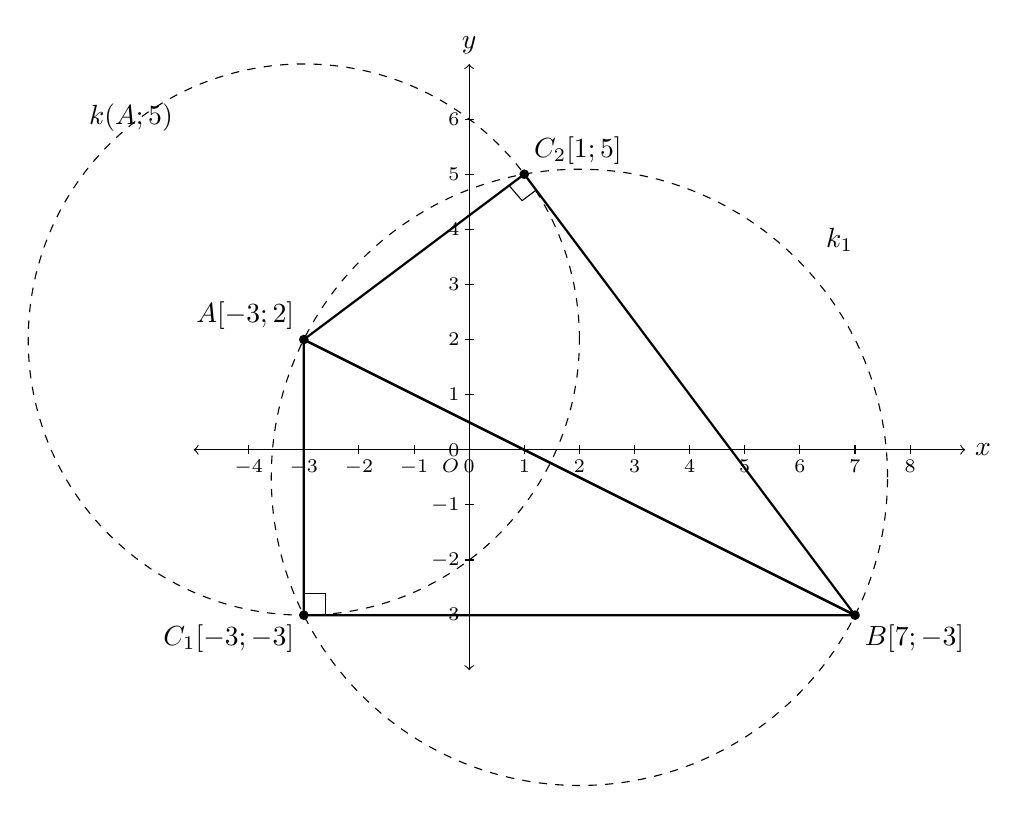
\begin{tikzpicture}[scale=0.7]

            % Osy
            \draw[<->, thin] (-5,0) -- (9,0) node[right] {$x$};
            \draw[<->, thin] (0,-4) -- (0,7) node[above] {$y$};
            \node[below left, font=\scriptsize] at (0,0) {$O$};

            % Značky na osách
            \foreach \x in {-4,-3,...,8}
            {
                \draw (\x,0.08) -- (\x,-0.08);
                \node[below, font=\scriptsize] at (\x,0) {$\x$};
            }

            \foreach \y in {-3,-2,...,6}
            {
                \draw (0.08,\y) -- (-0.08,\y);
                \node[left, font=\scriptsize] at (0,\y) {$\y$};
            }

            % Body
            \coordinate (A) at (-3,2);
            \coordinate (B) at (7,-3);
            \coordinate (C1) at (-3,-3);
            \coordinate (C2) at (1,5);
            \coordinate (M) at (2,-0.5);

            % Kružnice
            \draw[dashed] (A) circle (5);
            \draw[dashed] (M) circle ({sqrt(125)/2});

            % Trojúhelníky
            \draw[thick] (A) -- (B) -- (C1) -- cycle;
            \draw[thick] (A) -- (B) -- (C2) -- cycle;

            % Pravé úhly
            \draw (-3,-2.6) -- (-2.6,-2.6) -- (-2.6,-3);
            \draw (0.72,4.8) -- (0.96,4.52) -- (1.2,4.7);

            % Body
            \fill (A) circle (2.5pt) node[above left] {$A[-3;2]$};
            \fill (B) circle (2.5pt) node[below right] {$B[7;-3]$};
            \fill (C1) circle (2.5pt) node[below left] {$C_1[-3;-3]$};
            \fill (C2) circle (2.5pt) node[above right] {$C_2[1;5]$};

            % Popisky kružnic
            \node[above left] at (-5.2,5.6) {$k(A;5)$};
            \node[below right] at (6.3,4.2) {$k_1$};

        \end{tikzpicture}
        \caption{Body $C_1$ a $C_2$, pro které je trojúhelník $ABC$
        pravoúhlý s přeponou $AB$ a zároveň platí $|AC|=5$.}
        \label{fig:Right_triangle_given_hypotenuse_and_side}
    \end{figure}
\end{example}
\subsection{Odchylka přímek}
\label{subsec:Angle_between_lines}

V předchozích částech jsme určovali, zda jsou dvě přímky různoběžné,
rovnoběžné, totožné nebo kolmé. U různoběžných přímek však můžeme
zkoumat také velikost úhlu, pod kterým se protínají.

Směr přímky je určen jejím směrovým vektorem. Výpočet odchylky dvou
přímek proto navazuje na geometrický význam skalárního součinu,
kterému jsme se věnovali v části
\ref{subsubsec:Geometric_meaning_of_dot_product}. Budeme přitom
vycházet zejména ze vztahu \eqref{eq:dot_product_angle} pro výpočet
úhlu dvou vektorů, případně z jeho odvozené formy z poznámky \ref{rem:dot_product_angle}


\subsubsection{Geometrický význam odchylky přímek}
\label{subsubsec:Geometric_meaning_angle_lines}

Dvě různoběžné přímky vytvářejí ve svém průsečíku čtyři úhly.
Protilehlé úhly mají stejnou velikost a dva sousední úhly jsou
vedlejší, takže jejich součet je roven $\pi$.

Při určování odchylky přímek vybíráme menší z úhlů, které přímky
svírají. Jsou-li přímky kolmé, je jejich odchylka rovna
$\frac{\pi}{2}$. Rovnoběžné a totožné přímky mají odchylku rovnou
nule.

\begin{definition}\label{def:Angle_between_lines}
    \textbf{Odchylkou dvou přímek} $p$ a $q$ v rovině nazýváme číslo
    \[
        \varphi\in\left[0;\frac{\pi}{2}\right],
    \]
    které je u různoběžných přímek velikostí jejich ostrého nebo
    pravého úhlu.

    Pro rovnoběžné a totožné přímky definujeme
    \[
        \varphi=0.
    \]
\end{definition}

Odchylku přímek budeme značit
\[
    \varphi=\angle(p,q).
\]

\begin{figure}[H]
    \centering
    \begin{tikzpicture}[scale=1.05]

        \coordinate (O) at (0,0);

        % Přímky
        \draw[thin, <->] (-3,-1.5) -- (3,1.5)
            node[above right] {$p$};
        \draw[thin, <->] (-2.6,2.2) -- (2.6,-2.2)
            node[below right] {$q$};

        % Průsečík
        \fill (O) circle (2.3pt) node[below left] {$P$};

        % Směrové vektory
        \draw[vector] (0.4,0.2) -- (1.8,0.9)
            node[midway, above, sloped] {$\vec{u}$};
        \draw[vector] (0.35,-0.30) -- (1.55,-1.31)
            node[midway, below, sloped] {$\vec{v}$};

        % Oblouk odchylky
        \draw[->]
            (0.85,0.425)
            arc[start angle=26.565, end angle=-40.236, radius=0.95];

        \node[right] at (0.92,-0.08) {$\varphi$};

    \end{tikzpicture}
    \caption{Odchylka přímek je velikost menšího úhlu, který přímky
    svírají.}
    \label{fig:Angle_between_lines}
\end{figure}

Úhel dvou vektorů může nabývat hodnot od $0$ do $\pi$. Odchylka
přímek však nepřesahuje $\frac{\pi}{2}$. Navíc můžeme směrový vektor
přímky nahradit jeho opačným vektorem, aniž bychom změnili směr
přímky. Výpočet odchylky proto nesmí záviset na zvolené orientaci
směrových vektorů.


\subsubsection{Odchylka pomocí směrových vektorů}
\label{subsubsec:Angle_lines_direction_vectors}

Uvažujme přímky $p$ a $q$ s nenulovými směrovými vektory
\[
    \vec{u}_p=(u_1;u_2),
    \qquad
    \vec{u}_q=(v_1;v_2).
\]

Pro úhel $\alpha\in[0;\pi]$ jejich směrových vektorů platí
\[
    \cos\alpha
    =
    \frac{\vec{u}_p\cdot\vec{u}_q}
    {|\vec{u}_p|\,|\vec{u}_q|}.
\]

Je-li úhel $\alpha$ ostrý nebo pravý, je přímo odchylkou přímek.
Je-li $\alpha$ tupý, je odchylkou přímek vedlejší úhel
\[
    \varphi=\pi-\alpha.
\]
Pro jejich kosiny platí
\[
    \cos(\pi-\alpha)=-\cos\alpha.
\]

Obě možnosti můžeme spojit pomocí absolutní hodnoty skalárního
součinu. Pro odchylku přímek tedy platí
\begin{equation}\label{eq:Angle_lines_direction_vectors}
        \cos\varphi
    =
    \frac{
        \left|\vec{u}_p\cdot\vec{u}_q\right|
    }
    {
        |\vec{u}_p|\,|\vec{u}_q|
    }.
\end{equation}

Po rozepsání souřadnic směrových vektorů dostáváme
\begin{equation}\label{eq:Angle_lines_direction_vectors_coordinates}
    \cos\varphi
    =
    \frac{
        |u_1v_1+u_2v_2|
    }
    {
        \sqrt{u_1^2+u_2^2}\,
        \sqrt{v_1^2+v_2^2}
    }.
\end{equation}

Samotnou odchylku určíme pomocí funkce arkus kosinus:
\begin{equation}\label{eq:Angle_lines_arccos}
    \varphi
    =
    \arccos
    \left(
        \frac{
            \left|\vec{u}_p\cdot\vec{u}_q\right|
        }
        {
            |\vec{u}_p|\,|\vec{u}_q|
        }
    \right).
\end{equation}

\begin{remark}\label{rem:Absolute_value_angle_lines}
    Absolutní hodnota v čitateli zajišťuje dvě důležité vlastnosti:

    \begin{itemize}
        \item výsledná odchylka nepřesáhne $\frac{\pi}{2}$;
        \item výsledek nezávisí na orientaci směrových vektorů.
    \end{itemize}

    Nahradíme-li například vektor $\vec{u}_p$ opačným vektorem
    $-\vec{u}_p$, změní se znaménko skalárního součinu, ale jeho
    absolutní hodnota zůstane stejná.
\end{remark}

Ze vztahu \eqref{eq:Angle_lines_direction_vectors} přímo plynou známé
zvláštní případy:

\[
\begin{array}{c|c|c}
    \text{podmínka}
    &
    \cos\varphi
    &
    \text{vzájemná poloha}
    \\
    \hline
    \vec{u}_p=k\vec{u}_q,\ k\neq0
    &
    1
    &
    \varphi=0
    \\[1mm]
    \vec{u}_p\cdot\vec{u}_q=0
    &
    0
    &
    \varphi=\frac{\pi}{2}
\end{array}
\]

Rovnoběžné a totožné přímky mají odchylku $0$, zatímco kolmé přímky
mají odchylku $\frac{\pi}{2}$.

\begin{example}\label{exa:Angle_parametric_lines}
    Určete odchylku přímek
    \[
        \begin{aligned}
            p:\quad x&=1+2t,\\
                     y&=3-3t,
                     \qquad t\in\mathbb{R},
        \end{aligned}
    \]
    a
    \[
        \begin{aligned}
            q:\quad x&=2-s,\\
                     y&=3+s,
                     \qquad s\in\mathbb{R}.
        \end{aligned}
    \]

    Z parametrických vyjádření získáme směrové vektory
    \[
        \vec{u}_p=(2;-3),
        \qquad
        \vec{u}_q=(-1;1).
    \]

    Jejich skalární součin je
    \[
        \vec{u}_p\cdot\vec{u}_q
        =
        (2;-3)\cdot(-1;1)
        =
        -2-3
        =
        -5.
    \]

    Velikosti směrových vektorů jsou
    \[
        |\vec{u}_p|
        =
        \sqrt{2^2+(-3)^2}
        =
        \sqrt{13}
    \]
    a
    \[
        |\vec{u}_q|
        =
        \sqrt{(-1)^2+1^2}
        =
        \sqrt2.
    \]

    Dosadíme do vztahu
    \eqref{eq:Angle_lines_direction_vectors}:
    \begin{align*}
        \cos\varphi
        &=
        \frac{|-5|}{\sqrt{13}\sqrt2}\\
        &=
        \frac{5}{\sqrt{26}}.
    \end{align*}

    Odtud
    \[
        \varphi
        =
        \arccos\left(\frac{5}{\sqrt{26}}\right)
        \doteq
        11{,}31^\circ.
    \]

    Odchylka přímek je přibližně
    \[
        \varphi\doteq11^\circ19'.
    \]
\end{example}


\subsubsection{Odchylka přímek zadaných obecnými rovnicemi}
\label{subsubsec:Angle_general_lines}

Uvažujme přímky zadané obecnými rovnicemi
\[
    p:\quad a_1x+b_1y+c_1=0
\]
a
\[
    q:\quad a_2x+b_2y+c_2=0.
\]

Jejich normálové vektory jsou
\[
    \vec{n}_p=(a_1;b_1),
    \qquad
    \vec{n}_q=(a_2;b_2).
\]

Obě přímky otočíme o pravý úhel, zvolíme-li místo nich přímky ve
směru jejich normálových vektorů. Otočení obou směrů o stejný úhel
nezmění jejich vzájemnou odchylku. Odchylka přímek $p$ a $q$ je proto
stejná jako odchylka jejich normálových vektorů.

Můžeme tedy použít vztah
\begin{equation}\label{eq:Angle_general_lines}
    \cos\varphi
    =
    \frac{
        |a_1a_2+b_1b_2|
    }
    {
        \sqrt{a_1^2+b_1^2}\,
        \sqrt{a_2^2+b_2^2}
    }.
\end{equation}

Absolutní členy $c_1$ a $c_2$ se ve vzorci nevyskytují, protože
ovlivňují polohu přímek, nikoli jejich směr.

\begin{figure}[H]
    \centering
    \begin{tikzpicture}[scale=1.0]

        \coordinate (O) at (0,0);

        % Přímky
        \draw[thin, <->] (-3,-1.25) -- (3,1.25)
            node[above right] {$p$};
        \draw[thin, <->] (-2.7,2.0) -- (2.7,-2.0)
            node[below right] {$q$};

        % Normálové vektory z průsečíku
        \draw[vector] (O) -- (-0.7,1.7)
            node[midway, left] {$\vec{n}_p$};
        \draw[vector] (O) -- (1.25,1.7)
            node[midway, right] {$\vec{n}_q$};

        % Oblouky
        \draw[->]
            (0.75,0.313)
            arc[start angle=22.62, end angle=-36.53, radius=0.81];
        \node[right] at (0.82,-0.05) {$\varphi$};

        \draw[->]
            (-0.32,0.78)
            arc[start angle=112.38, end angle=53.67, radius=0.84];
        \node[above] at (0.05,0.86) {$\varphi$};

        \fill (O) circle (2.2pt);

    \end{tikzpicture}
    \caption{Odchylka dvou přímek je stejná jako odchylka jejich
    normálových vektorů.}
    \label{fig:Angle_general_lines_normals}
\end{figure}

\begin{example}\label{exa:Angle_general_line_equations}
    Určete odchylku přímek $p: 2x-y+3=0$ a $q:3x+2y-1=0$.

    Normálové vektory přímek jsou
    \[
        \vec{n}_p=(2;-1),
        \qquad
        \vec{n}_q=(3;2).
    \]

    Jejich skalární součin je
    \[
        \vec{n}_p\cdot\vec{n}_q
        =
        (2;-1)\cdot(3;2)
        =
        6-2
        =
        4.
    \]

    Velikosti normálových vektorů jsou
    \[
        |\vec{n}_p|=\sqrt{2^2+(-1)^2}=\sqrt5
    \]
    a
    \[
        |\vec{n}_q|=\sqrt{3^2+2^2}=\sqrt{13}.
    \]

    Dosadíme do vztahu \eqref{eq:Angle_general_lines}:
    \[
        \cos\varphi
        =
        \frac{4}{\sqrt5\sqrt{13}}
        =
        \frac{4}{\sqrt{65}}.
    \]

    Odtud
    \[
        \varphi
        =
        \arccos\left(\frac{4}{\sqrt{65}}\right)
        \doteq
        60{,}26^\circ.
    \]

    Odchylka přímek je přibližně
    \[
        \varphi\doteq60^\circ15'.
    \]
\end{example}


\subsubsection{Odchylka přímek ve směrnicovém tvaru}
\label{subsubsec:Angle_slope_lines}

Uvažujme dvě nesvislé přímky ve směrnicovém tvaru
\[
    p:\quad y=k_1x+q_1
\]
a
\[
    q:\quad y=k_2x+q_2.
\]

Jako jejich směrové vektory můžeme zvolit
\[
    \vec{u}_p=(1;k_1),
    \qquad
    \vec{u}_q=(1;k_2).
\]

Dosazením do vztahu
\eqref{eq:Angle_lines_direction_vectors} získáme
\begin{equation}\label{eq:Angle_slope_lines_cosine}
    \cos\varphi
    =
    \frac{|1+k_1k_2|}
    {\sqrt{1+k_1^2}\sqrt{1+k_2^2}}.
\end{equation}

Odchylku můžeme určit také pomocí směrových úhlů přímek. Platí-li
\[
    k_1=\tan\alpha_1
    \qquad\text{a}\qquad
    k_2=\tan\alpha_2,
\]
pak s využitím vztahu pro tangens rozdílu dostáváme
\begin{equation}\label{eq:Angle_slope_lines_tangent}
    \tan\varphi
    =
    \left|
        \frac{k_2-k_1}{1+k_1k_2}
    \right|.
\end{equation}

Tento vztah můžeme použít, pokud
\[
    1+k_1k_2\neq0.
\]

Jestliže
\[
    1+k_1k_2=0,
\]
platí
\[
    k_1k_2=-1,
\]
a přímky jsou kolmé. Jejich odchylka je tedy
\[
    \varphi=\frac{\pi}{2}.
\]

Absolutní členy $q_1$ a $q_2$ opět nemají na odchylku vliv.

\begin{remark}\label{rem:Alternative_method_angle_slope_lines}
    Vztahy \eqref{eq:Angle_slope_lines_cosine}
    a \eqref{eq:Angle_slope_lines_tangent} umožňují určit odchylku
    přímo ze směrnic obou přímek.

    Tyto vztahy však není nutné pamatovat jako další samostatné
    vzorce. Obě přímky můžeme nejprve převést ze směrnicového tvaru
    na obecné rovnice a následně použít již známý vztah
    \eqref{eq:Angle_general_lines} pro výpočet odchylky pomocí
    normálových vektorů.

    Přímku
    \[
        y=kx+q
    \]
    převedeme na obecnou rovnici ve tvaru
    \[
        kx-y+q=0.
    \]
    Jejím normálovým vektorem je potom
    \[
        \vec{n}=(k;-1).
    \]

    Oba postupy vedou ke stejnému výsledku. Přímý vztah využívající
    směrnice představuje pouze zkrácení výpočtu.
\end{remark}

\begin{example}\label{exa:Angle_slope_intercept_lines}
    Určete odchylku přímek
    \[
        p:\quad y=2x-1
    \]
    a
    \[
        q:\quad y=\frac12x+3.
    \]

    Směrnice přímek jsou
    \[
        k_1=2,
        \qquad
        k_2=\frac12.
    \]

    Použijeme vztah
    \eqref{eq:Angle_slope_lines_tangent}:
    \begin{align*}
        \tan\varphi
        &=
        \left|
            \frac{\frac12-2}
            {1+2\cdot\frac12}
        \right|\\
        &=
        \left|
            \frac{-\frac32}{2}
        \right|\\
        &=
        \frac34.
    \end{align*}

    Odtud
    \[
        \varphi
        =
        \arctan\left(\frac34\right)
        \doteq
        36{,}87^\circ.
    \]

    Odchylka přímek je přibližně
    \[
        \varphi\doteq36^\circ52'.
    \]
\end{example}

\begin{remark}\label{rem:Vertical_line_angle}
    Směrnicový tvar nelze použít pro svislou přímku. Je-li alespoň
    jedna z přímek svislá, určíme odchylku pomocí směrových nebo
    normálových vektorů. Pro svislou přímku můžeme zvolit například
    směrový vektor
    \[
        \vec{u}=(0;1).
    \]
\end{remark}

\begin{example}\label{exa:Angle_slope_lines_by_conversion}
    Určete odchylku přímek $p: y=\frac{3}{4}x-2$ a $q: y=-\frac{1}{2}x+1$.

    Přímky jsou zadány ve směrnicovém tvaru. Místo přímého použití
    vztahu pro jejich směrnice je nejprve převedeme na obecné rovnice
    a následně použijeme vztah \eqref{eq:Angle_general_lines}.

    Nejprve upravíme rovnici přímky $p$:
    \begin{align*}
        y&=\frac{3}{4}x-2,\\
        \frac{3}{4}x-y-2&=0.
    \end{align*}

    Abychom odstranili zlomek, vynásobíme rovnici číslem $4$:
    \[
        p:\quad 3x-4y-8=0.
    \]

    Normálový vektor přímky $p$ je tedy
    \[
        \vec{n}_p=(3;-4).
    \]

    Nyní převedeme na obecnou rovnici přímku $q$:
    \begin{align*}
        y&=-\frac{1}{2}x+1,\\
        \frac{1}{2}x+y-1&=0.
    \end{align*}

    Po vynásobení rovnice číslem $2$ dostáváme
    \[
        q:\quad x+2y-2=0.
    \]

    Normálový vektor přímky $q$ je
    \[
        \vec{n}_q=(1;2).
    \]

    Vypočítáme skalární součin normálových vektorů:
    \[
        \vec{n}_p\cdot\vec{n}_q
        =
        (3;-4)\cdot(1;2)
        =
        3-8
        =
        -5.
    \]

    Velikosti normálových vektorů jsou
    \[
        |\vec{n}_p|
        =
        \sqrt{3^2+(-4)^2}
        =
        5
    \]
    a
    \[
        |\vec{n}_q|
        =
        \sqrt{1^2+2^2}
        =
        \sqrt5.
    \]

    Dosadíme do vztahu \eqref{eq:Angle_general_lines}:
    \begin{align*}
        \cos\varphi
        &=
        \frac{
            |\vec{n}_p\cdot\vec{n}_q|
        }
        {
            |\vec{n}_p|\,|\vec{n}_q|
        }\\
        &=
        \frac{|-5|}{5\sqrt5}\\
        &=
        \frac{1}{\sqrt5}.
    \end{align*}

    Odtud
    \[
        \varphi
        =
        \arccos\left(\frac{1}{\sqrt5}\right)
        \doteq
        63{,}43^\circ.
    \]

    Odchylka přímek je přibližně
    \[
        \varphi\doteq63^\circ26'.
    \]

    Ke stejnému výsledku bychom dospěli také přímým použitím vztahu
    \eqref{eq:Angle_slope_lines_tangent}. Převod na obecné rovnice
    nám však umožnil použít již známý postup založený na normálových
    vektorech.
\end{example}


\subsubsection{Přímky zadané různými způsoby}
\label{subsubsec:Angle_lines_mixed_forms}

Jsou-li přímky zadány různými způsoby, není nutné vždy převádět celé
jejich rovnice do stejného tvaru. Často stačí z každého zápisu získat
směrový nebo normálový vektor a následně použít vztah
\eqref{eq:Angle_lines_direction_vectors}.

Můžeme postupovat například takto:

\[
\begin{array}{c|c}
    \text{zadání přímky}
    &
    \text{vhodný vektor}
    \\
    \hline
    \text{dva body }A,B
    &
    \overrightarrow{AB}=B-A
    \\[1mm]
    \text{parametrické vyjádření}
    &
    \vec{u}=(u_x;u_y)
    \\[1mm]
    \text{obecná rovnice }ax+by+c=0
    &
    \vec{n}=(a;b)
    \text{ nebo }
    \vec{u}=(-b;a)
    \\[1mm]
    \text{směrnicový tvar }y=kx+q
    &
    \vec{u}=(1;k)
\end{array}
\]

Pro výpočet musí být oba zvolené vektory stejného typu: buď dva
směrové, nebo dva normálové vektory.

\begin{example}\label{exa:Angle_line_through_points_and_general_line}
    Jsou dány body
    \[
        A[-3;1],
        \qquad
        B[1;2]
    \]
    a přímka
    \[
        p:\quad 2x-y+3=0.
    \]

    Určete odchylku přímky $AB$ a přímky $p$.

    Směrový vektor přímky $AB$ je
    \[
        \vec{u}_{AB}
        =
        \overrightarrow{AB}
        =
        (1-(-3);2-1)
        =
        (4;1).
    \]

    Z obecné rovnice přímky $p$ získáme normálový vektor
    \[
        \vec{n}_p=(2;-1).
    \]
    K němu zvolíme kolmý směrový vektor
    \[
        \vec{u}_p=(1;2).
    \]

    Skalární součin směrových vektorů je
    \[
        \vec{u}_{AB}\cdot\vec{u}_p
        =
        (4;1)\cdot(1;2)
        =
        4+2
        =
        6.
    \]

    Jejich velikosti jsou
    \[
        |\vec{u}_{AB}|=\sqrt{4^2+1^2}=\sqrt{17}
    \]
    a
    \[
        |\vec{u}_p|=\sqrt{1^2+2^2}=\sqrt5.
    \]

    Proto
    \[
        \cos\varphi
        =
        \frac{6}{\sqrt{17}\sqrt5}
        =
        \frac{6}{\sqrt{85}}.
    \]

    Odtud
    \[
        \varphi
        =
        \arccos\left(\frac{6}{\sqrt{85}}\right)
        \doteq
        49{,}40^\circ.
    \]

    Odchylka přímek je přibližně
    \[
        \varphi\doteq49^\circ24'.
    \]
\end{example}





\subsubsection{Přímka procházející bodem s danou odchylkou}
\label{subsubsec:Line_through_point_given_angle}

Úlohu můžeme také obrátit. Známe-li přímku $p$, bod $Q$ a požadovanou
odchylku $\varphi$, hledáme přímky procházející bodem $Q$, které
svírají s přímkou $p$ daný úhel.

Není-li požadovaná odchylka rovna nule ani pravému úhlu, existují
obvykle dvě takové přímky. Jedna vznikne otočením směru přímky $p$
o úhel $\varphi$ na jednu stranu a druhá otočením o tentýž úhel na
stranu opačnou.

\begin{example}\label{exa:Lines_through_point_given_angle}
    Je dána přímka $p:x-3y-2=0$ a bod $Q[1;1]$. Určete všechny
    přímky procházející bodem $Q$, jejichž odchylka od přímky $p$
    je $45^\circ$.

    Z obecné rovnice přímky $p$ získáme normálový vektor
    \[
        \vec{n}_p=(1;-3).
    \]
    Jako směrový vektor přímky $p$ můžeme zvolit
    \[
        \vec{u}_p=(3;1).
    \]

    Hledaná přímka $q$ prochází bodem $Q[1;1]$. Nejprve budeme
    předpokládat, že není svislá, a její směrový vektor zapíšeme jako
    \[
        \vec{u}_q=(1;k),
    \]
    kde $k$ je její směrnice.

    Pro odchylku $45^\circ$ musí platit
    \[
        \cos45^\circ
        =
        \frac{
            |\vec{u}_p\cdot\vec{u}_q|
        }
        {
            |\vec{u}_p|\,|\vec{u}_q|
        }.
    \]

    Po dosazení dostáváme
    \[
        \frac{\sqrt2}{2}
        =
        \frac{|3+k|}
        {\sqrt{10}\sqrt{1+k^2}}.
    \]

    Umocníme obě strany rovnice a postupně upravíme:
    \begin{align*}
        \frac12
        &=
        \frac{(3+k)^2}{10(1+k^2)},\\
        5(1+k^2)
        &=
        (3+k)^2,\\
        5+5k^2
        &=
        9+6k+k^2,\\
        4k^2-6k-4
        &=
        0,\\
        2k^2-3k-2
        &=
        0.
    \end{align*}

    Vyřešíme kvadratickou rovnici:
    \[
        (2k+1)(k-2)=0.
    \]

    Dostáváme dvě směrnice:
    \[
        k_1=2,
        \qquad
        k_2=-\frac12.
    \]

    \paragraph{První hledaná přímka}

    Přímka se směrnicí $k_1=2$ prochází bodem $Q[1;1]$. Použijeme
    bodově-směrnicový tvar (viz vztah \eqref{eq:Point_slope_line_equation}):
    \begin{align*}
        y-1&=2(x-1),\\
        y-1&=2x-2,\\
        2x-y-1&=0.
    \end{align*}

    První hledaná přímka je
    \[
        q_1:2x-y-1=0.
    \]

    Přímka $q_1$ společně s původní přímkou $p$ je znázorněna
    na obrázku~\ref{fig:First_line_through_point_given_angle}.
    Přímky se protínají v bodě
    \[
        P_1\left[\frac15;-\frac35\right]
    \]
    a jejich odchylka je $45^\circ$.

    \begin{figure}[H]
        \centering
        \begin{tikzpicture}[scale=0.85]

            % Osy
            \draw[<->, thin] (-3,0) -- (6,0) node[right] {$x$};
            \draw[<->, thin] (0,-3) -- (0,6) node[above] {$y$};
            \node[below left] at (0,0) {$O$};

            % Původní přímka p: y=(x-2)/3
            \draw[thin, <->]
                (-3,-5/3) -- (6,4/3)
                node[above right] {$p$};

            % První hledaná přímka q_1: y=2x-1
            \draw[thick, <->]
                (-1,-3) -- (3.5,6)
                node[above right] {$q_1$};

            % Bod Q
            \fill (1,1) circle (2.6pt)
                node[above left] {$Q[1;1]$};

            % Průsečík p a q_1
            \coordinate (Pone) at (0.2,-0.6);
            \fill (Pone) circle (2.2pt)
                node[below right] {$P_1$};

            % Odchylka 45 stupňů
            \draw[->]
                ($(Pone)+(0.75,0.25)$)
                arc[
                    start angle=18.435,
                    end angle=63.435,
                    radius=0.79
                ];

            \node[right] at (0.85,0.02) {$45^\circ$};

        \end{tikzpicture}
        \caption{První přímka $q_1$ procházející bodem $Q$ a svírající
        s přímkou $p$ úhel $45^\circ$.}
        \label{fig:First_line_through_point_given_angle}
    \end{figure}


    \paragraph{Druhá hledaná přímka}

    Pro směrnici $k_2=-\frac12$ dostáváme
    \begin{align*}
        y-1&=-\frac12(x-1),\\
        2y-2&=-x+1,\\
        x+2y-3&=0.
    \end{align*}

    Druhá hledaná přímka je
    \[
        q_2:x+2y-3=0.
    \]

    Na obrázku~\ref{fig:Second_line_through_point_given_angle} je
    nově sestrojená přímka $q_2$ znázorněna plnou čarou. První
    nalezená přímka $q_1$ je pro porovnání vyznačena čárkovaně.
    Přímky $p$ a $q_2$ se protínají v bodě
    \[
        P_2\left[\frac{13}{5};\frac15\right]
    \]
    a jejich odchylka je opět $45^\circ$.

    \begin{figure}[H]
        \centering
        \begin{tikzpicture}[scale=0.85]

            % Osy
            \draw[<->, thin] (-3,0) -- (6,0) node[right] {$x$};
            \draw[<->, thin] (0,-3) -- (0,6) node[above] {$y$};
            \node[below left] at (0,0) {$O$};

            % Původní přímka p
            \draw[thin, <->]
                (-3,-5/3) -- (6,4/3)
                node[above right] {$p$};

            % První řešení čárkovaně
            \draw[thick, dashed, <->]
                (-1,-3) -- (3.5,6)
                node[above right] {$q_1$};

            % Druhé řešení plnou čarou
            \draw[thick, <->]
                (-3,3) -- (6,-1.5)
                node[below right] {$q_2$};

            % Bod Q
            \fill (1,1) circle (2.6pt)
                node[above right] {$Q[1;1]$};

            % Průsečík p a q_2
            \coordinate (Ptwo) at (2.6,0.2);
            \fill (Ptwo) circle (2.2pt)
                node[above right] {$P_2$};

            % Odchylka 45 stupňů
            \draw[->]
                ($(Ptwo)+(0.72,-0.36)$)
                arc[
                    start angle=-26.565,
                    end angle=18.435,
                    radius=0.81
                ];

            \node[right] at (3.38,0.18) {$45^\circ$};

        \end{tikzpicture}
        \caption{Druhá přímka $q_2$ procházející bodem $Q$. První
        nalezená přímka $q_1$ je znázorněna čárkovaně.}
        \label{fig:Second_line_through_point_given_angle}
    \end{figure}

    Svislá přímka procházející bodem $Q$ má směrový vektor
    \[
        \vec{u}_s=(0;1).
    \]
    Pro její odchylku od přímky $p$ by platilo
    \[
        \cos\varphi
        =
        \frac{|(3;1)\cdot(0;1)|}
        {\sqrt{3^2+1^2}\sqrt{0^2+1^2}}
        =
        \frac{1}{\sqrt{10}}.
    \]
    Tato hodnota neodpovídá úhlu $45^\circ$, takže žádné další
    řešení nevzniká.

    Zadání splňují právě dvě přímky:
    \[
        q_1:2x-y-1=0
    \]
    a
    \[
        q_2:x+2y-3=0.
    \]

    Celková situace je znázorněna na obrázku
    \ref{fig:Lines_through_point_given_angle}. Původní přímka $p$
    je v obrázku zvýrazněna silnější čarou.

    \begin{figure}[H]
        \centering
        \begin{tikzpicture}[scale=1]

            % Osy
            \draw[<->, thin] (-4,0) -- (7,0) node[right] {$x$};
            \draw[<->, thin] (0,-4) -- (0,7) node[above] {$y$};
            \node[below left] at (0,0) {$O$};

            % Hodnoty na ose x
            \foreach \x in {-3,-2,-1,1,2,3,4,5,6}
            {
                \draw (\x,0.10) -- (\x,-0.10);
                \node[below, font=\scriptsize] at (\x,0) {$\x$};
            }

            % Hodnoty na ose y
            \foreach \y in {-3,-2,-1,1,2,3,4,5,6}
            {
                \draw (0.10,\y) -- (-0.10,\y);
                \node[left, font=\scriptsize] at (0,\y) {$\y$};
            }

            % Původní přímka p zvýrazněně
            \draw[very thick, <->]
                (-4,-2) -- (7,5/3)
                node[above right] {$p$};

            % Hledané přímky
            \draw[thick, <->]
                (-1.5,-4) -- (4,7)
                node[above right] {$q_1$};

            \draw[thick, <->]
                (-4,3.5) -- (7,-2)
                node[below right] {$q_2$};

            % Bod Q
            \fill (1,1) circle (3pt)
                node[above right] {$Q[1;1]$};

            % Průsečíky
            \coordinate (Pone) at (0.2,-0.6);
            \coordinate (Ptwo) at (2.6,0.2);

            \fill (Pone) circle (2.2pt)
                node[below left] {$P_1$};

            \fill (Ptwo) circle (2.2pt)
                node[above right] {$P_2$};

            % První úhel
            \draw[->]
                ($(Pone)+(0.72,0.24)$)
                arc[
                    start angle=18.435,
                    end angle=63.435,
                    radius=0.76
                ];

            \node[above right, font=\small] at (0.82,0.00) {$45^\circ$};

            % Druhý úhel
            \draw[->]
                ($(Ptwo)+(0.68,-0.34)$)
                arc[
                    start angle=-26.565,
                    end angle=18.435,
                    radius=0.76
                ];

            \node[right, font=\small] at (3.34,0.18) {$45^\circ$};

        \end{tikzpicture}
        \caption{Přímky $q_1$ a $q_2$ procházející bodem $Q$, jejichž
        odchylka od zvýrazněné přímky $p$ je $45^\circ$.}
        \label{fig:Lines_through_point_given_angle}
    \end{figure}
\end{example}


\begin{remark}\label{rem:Summary_angle_between_lines}
    Při výpočtu odchylky přímek není nutné pamatovat několik
    nesouvisejících vzorců. Základním postupem je vždy určit dva
    směrové vektory a použít vztah
    \eqref{eq:Angle_lines_direction_vectors}.

    Vzorce pro obecné rovnice a směrnicové tvary jsou pouze jeho
    upravenými podobami, které umožňují pracovat přímo se zadaným
    tvarem přímek.
\end{remark}
